% LaTeX source for book ``代数学方法'' in Chinese
% Copyright 2018  李文威 (Wen-Wei Li).
% Permission is granted to copy, distribute and/or modify this
% document under the terms of the Creative Commons
% Attribution 4.0 International (CC BY 4.0)
% http://creativecommons.org/licenses/by/4.0/

% To be included
\chapter{域的赋值}
按后见之明, 赋值在域论中是自然的对象, 例如
\begin{itemize}
	\item 给定了素数 $p$, 对域 $\Q$ 的任意元素 $x \neq 0$ 可以考虑 $p$ 在其素因子分解中出现的次数 $v_p(x)$, 另外定义 $v_p(0)=\infty$;
	\item 类似地, 对于 Riemann 曲面 $X$ 上的一点 $x$ 及 $X$ 上的亚纯函数 $f$, 可考虑 $f$ 在 $x$ 处的消没次数 $v_x(f) \in \Z \sqcup \{\infty\}$.
\end{itemize}
推而广之, 赋值论考虑满足一定条件的函数 $v: A \to \Gamma \sqcup \{\infty\}$, 其中 $A$ 是交换环而 $\Gamma$ 是全序交换群 (例如加法群 $\Z$, $\R$). 容许一般的全序交换群是 Krull 的创见, 最常见的 $\Gamma \subset \R$ 情形则称为秩 $1$ 赋值. 赋值自然地引向拓扑结构, 极限和完备性, 如 $p$-进数域 $\Q_p$ 正是 $\Q$ 对 $v_p$ 的完备化. 完备化为域论的研究提供了一系列解析工具, 譬如多项式求根时使用的 Hensel 引理 (定理 \ref{prop:Hensel-lemma}). 这些概念在代数数论和代数几何中顺理成章, 本书只予以粗浅的介绍.

涵摄秩 $1$ 赋值而稍加广泛的概念是绝对值, 譬如对 $\Q$ 可取 $|\cdot|_p := p^{-v_p(\cdot)}$ ($p$ 为素数) 或寻常的绝对值 $|\cdot|_\infty$, 相关的分类定理是优美而富于技巧的.

本章最后介绍的 Witt 向量是将特征 $p > 0$ 的完全域提升到特征 $0$ 的有力工具, 应用包括了代数几何中特征 $p$ 代数簇的上同调理论等等. 它的原初设想很自然: 如何从 $p$-进制展开来理解 $\Q_p$ 及其非分歧扩张的代数结构? E.\ Witt 对此作出了初等又精妙的回答.

\begin{wenxintishi}
	首先 \S\ref{sec:filters} 是一些关于拓扑的预备知识和定义, 如读者对完备化已有很好的掌握则可略过, 借机学习 Cartan 的滤子语言也不无益处. 我们在 \S\ref{sec:Krull-valuation} 和 \S\ref{sec:valued-field} 探讨取值在一般全序交换群 $\Gamma$ 中的赋值, 亦即 Krull 赋值, 然而在许多应用中只需要秩 $1$ 情形.
	
	\S\ref{sec:absolute-value} 旨在讨论绝对值及其分类. 随后 \S\ref{sec:closed-unit-disc} 把焦点转向环 $K^\circ \lrangle{t}$, 或者按几何视角即单位闭圆盘的情形; 这是非 Archimedes 解析几何的基本样板, 同时是一窥赋值论面貌的有趣例子.

	赋值延拓的讨论 (\S\ref{sec:valuation-ext-1} 和 \S\ref{sec:valuation-ext-2}) 较冗长而且需要技巧, 尤其是在非完备的情形, 尽管成果终归是单纯的. 相关理论常见于代数数论的教科书, 如 \cite{Lai16}; 在此之所以不避重复地研究, 主要缘于我们认为这是自然的理势. 请读者按自己的兴趣和时间来斟酌. 相关讨论参考了 \cite[Chapter XII]{Lang02} 和 \cite[Chapter II]{Neu99} 的进路.
\end{wenxintishi}

\section{滤子}\label{sec:filters}
滤子的概念肇端于 H.\ Cartan, 详述见 \cite{Bou-Top1}. 它用于收敛性和完备化的探究是一套特别精练的语言, 在数理逻辑领域也多有应用. 本节需要点集拓扑学的一些基础知识.

\begin{definition}\index{luzi@滤子 (filter)}
	非空集 $X$ 上的一个\emph{滤子}意谓具以下条件的子集族 $\mathfrak{F} \subset P(X)$, $\mathfrak{F} \neq \emptyset$:
	\begin{enumerate}[\bfseries {F}.1]
		\item 若 $A, B \in \mathfrak{F}$, 则 $A \cap B \in \mathfrak{F}$ (向下封闭性);
		\item 若 $A \in \mathfrak{F}$ 而 $X \supset A' \supset A$, 则 $A' \in \mathfrak{F}$ (向上封闭性);
		\item $\emptyset \notin \mathfrak{F}$.
	\end{enumerate}
	若子集族 $\mathfrak{B} \neq \emptyset$ 具较弱的条件如下, 则称之为 $X$ 上的\emph{滤子基}:
	\begin{enumerate}[\bfseries {FB}.1]
		\item 若 $A, B \in \mathfrak{B}$, 则存在 $C \in \mathfrak{B}$ 使得 $C \subset A \cap B$,
		\item $\emptyset \notin \mathfrak{B}$.
	\end{enumerate}
	对于滤子基 $\mathfrak{B}$, 称 $\mathfrak{F} := \{ F \subset X: \exists B \in \mathfrak{B},\; F \supset B \}$ 为 $\mathfrak{B}$ 生成的滤子, 而称 $\mathfrak{B}$ 为 $\mathfrak{F}$ 的一个基. 若 $\mathfrak{F} \subset \mathfrak{F}'$ 皆是 $X$ 上的滤子, 则称 $\mathfrak{F}'$ 是 $\mathfrak{F}$ 的\emph{加细}.
\end{definition}

\begin{example}\label{eg:sequence-as-filter}
	设 $(x_k)_{k=1}^\infty$ 为 $X$ 中的序列. 定义 $\mathfrak{F}$ 为全体满足下述条件之子集 $E \subset X$
	\[ \exists N \geq 1, \quad k \geq N \implies x_k \in E . \]
	易对 $\mathfrak{F}$ 验证滤子的条件; 全体形如 $\{ x_k, x_{k+1}, \ldots\}$ 的子集 ($k \geq N$ 任取, 其中 $N \geq 1$ 是某个选定的整数) 则构成 $\mathfrak{F}$ 的基.
\end{example}

\begin{example}\label{eg:nbd-filter}
	设 $X$ 为拓扑空间. 对每个 $x \in X$ 取 $\mathfrak{N}_x$ 为 $x$ 的全体邻域: 请回忆 $E \subset X$ 是 $x$ 的邻域相当于存在开集 $U$ 使得 $x \in U \subset E$. 易见 $\mathfrak{N}_x$ 构成 $X$ 上的滤子. 点集拓扑学中所谓 $x$ 的邻域基 (见 \cite[定义 2.6.3]{Xiong}) 无非是滤子 $\mathfrak{N}_x$ 的基.

	事实上 $\{ \mathfrak{N}_x : x \in X \}$ 完全确定了 $X$ 的拓扑结构, 这是因为 $V \subset X$ 为开集当且仅当 $V$ 是它每一点的邻域. 甚至能证明给定 $X$ 上的拓扑相当于给定一族滤子 $\{ \mathfrak{N}_x  : x \in X\}$, 使得对每个 $x$ 皆有
	\begin{compactitem}
		\item 若 $E \in \mathfrak{N}_x$, 则 $x \in E$;
		\item 若 $E \in \mathfrak{N}_x$, 则存在 $F \in \mathfrak{N}_x$ 使得 $F \subset E$ 且 $y \in F \implies F \in \mathfrak{N}_y$.
	\end{compactitem}
	对应关系由 $\mathfrak{N}_x = \{E : x\; \text{的邻域}\}$ 刻画. 详见 \cite[定理 2.3.3]{Xiong}. 因此拓扑结构亦可用滤子的语言改写. 我们马上会看到这套进路的长处.
\end{example}

回顾定义 \ref{def:topological-group} 谈及的拓扑群. 本节只考虑 Hausdorff 交换拓扑群, 群运算写作加法. 这些群构成范畴 $\cate{TopAb}$, 其态射取作连续群同态. 准此要领, 可以得到 Hausdorff 拓扑环范畴 $\cate{TopRing}$ 和 Hausdorff 拓扑域范畴 $\cate{TopField}$; 对于拓扑域, 我们要求乘法取逆 $K^\times \to K^\times$ 也是连续的. 进一步, 还可以谈论拓扑环上的拓扑模. \index{tuopuhuan} \index[sym1]{TopAb@$\cate{TopAb}$, $\cate{TopRing}$, $\cate{TopField}$} \index{tuopuqun}

以下固定拓扑空间 $X$, 相应的邻域滤子仍记为 $\mathfrak{N}_x$, $x \in X$. 根据例 \ref{eg:sequence-as-filter}, 任意序列 $(x_k)_{k=1}^\infty$ 都生成 $X$ 上的滤子, 而 $X$ 上的滤子可视作序列的某种推广.
\begin{description}
	\item[收敛性] 称 $X$ 上的滤子基 $\mathfrak{F}$ 收敛于 $x \in X$, 如果每个 $x$ 的邻域都包含某个 $F \in \mathfrak{F}$, 写作 $\mathfrak{F} \to x$; 当 $\mathfrak{F}$ 是滤子时, 这等价于 $\mathfrak{F}$ 是 $\mathfrak{N}_x$ 的加细. 此时 \textbf{FB.1} 蕴涵 $x$ 属于每个 $F \in \mathfrak{F}$ 的闭包. 请读者检查这一切和序列情形是兼容的.
	\item[分离性] 空间 $X$ 是 Hausdorff 空间当且仅当每个滤子至多收敛到一个点.
	\item[连续性] 对于函数 $f: X \to Y$ 和 $X$ 上的滤子 $\mathfrak{F}$, 置
		\[ f\mathfrak{F} := \left\{ F \subset Y: \exists E \in \mathfrak{F},\; F \supset f(E) \right\}, \]
		这是 $Y$ 上的滤子 (理由: $f(A) \cap f(B) \supset f(A \cap B)$). 事实: $f$ 连续当且仅当对每个 $x \in X$ 都有 $(\mathfrak{F} \to x) \implies (f\mathfrak{F} \to f(x))$.
	\item[Cauchy 滤子] 设 $(A, +)$ 是 Hausdorff 交换拓扑群, 此时 \index{luzi!Cauchy}
		\[ \mathfrak{N}_0 + x = \mathfrak{N}_x = x + \mathfrak{N}_0, \quad -\mathfrak{N}_0 = \mathfrak{N}_0. \]
		称 $A$ 上的滤子 $\mathfrak{F}$ 是 \emph{Cauchy 滤子}, 如果对任何邻域 $U \in \mathfrak{N}_0$ 皆存在 $E \in \mathfrak{F}$ 使得
		\[ E-E := \left\{x-y: x,y \in E \right\} \subset U. \]
		以同样性质定义 Cauchy 滤子基, 它们生成 Cauchy 滤子.
		\begin{compactenum}[(a)]
			\item 由定义立见 Cauchy 滤子的加细仍是 Cauchy 滤子.
			\item 对于任意 $x \in A$, 邻域族 $\mathfrak{N}_x$ 是 Cauchy 滤子: 诚然, 根据群运算的连续性, 对给定的 $U$ 可取 $E_0 \in \mathfrak{N}_0$ 使得 $E_0 - E_0 \subset U$, 从而 $E := x + E_0 \in \mathfrak{N}_x$ 满足于 $E-E = E_0 - E_0 \subset U$.
			\item 综上, 收敛滤子 $\mathfrak{F}$ 必为 Cauchy 滤子, 因为此时 $\mathfrak{F}$ 是某 $\mathfrak{N}_x$ 的加细.
		\end{compactenum}
		此外, 拓扑群的连续同态 $f: A \to B$ 映任意 Cauchy 滤子 $\mathfrak{F}$ 为 Cauchy 滤子 $f\mathfrak{F}$: 给定 $0 \in B$ 的邻域 $V$, 以 $f$ 的连续性取 $0 \in A$ 的邻域 $U$ 使得 $f(U) \subset V$, 再取 $E \in \mathfrak{F}$ 使得 $E-E \subset U$, 于是 $F := f(E) \in f\mathfrak{F}$ 满足
		\[ F - F = f(E-E) \subset f(U) \subset V. \]
		同样地, 请读者验证这一切兼容于 Cauchy 序列的经典概念.
	\item[完备性] 如果交换拓扑群 $A$ 中的每个 Cauchy 滤子都收敛, 则称 $A$ 是\emph{完备}的. 一般只对 Hausdorff 空间探讨完备性.
\end{description}

若对所有 $x \in X$, 滤子 $\mathfrak{N}_x$ 皆有可数基, 则称 $X$ 满足第一可数公理. 这类例子包括了习见的度量空间 $(X, d)$, 因所有以 $x$ 为球心, $d$-半径为 $\frac{1}{2}, \frac{1}{3}, \ldots$ 的开球给出一族可数基. 在第一可数公理下, 前述拓扑性质的刻画中可以用序列代替滤子, 这是点集拓扑的标准知识, 详参 \cite[\S 5.1]{Xiong}.

对于 Hausdorff 交换拓扑群 $A$, 其\emph{完备化}指的是范畴 $\cate{TopAb}$ 中的一个态射 $\iota: A \to \hat{A}$, 满足于 \index{wanbeihua}
\begin{compactenum}[(\bfseries {CO}.1)]
	\item $\iota: A \to \iota(A)$ 为同胚,
	\item $\iota(A) \subset \hat{A}$ 稠密,
	\item $\hat{A}$ 在 Cauchy 滤子意义下完备.
\end{compactenum}
命题 \ref{prop:completion-ring-characterization} 将证明这组性质唯一刻画了 $(\hat{A}, \iota)$. 存在性的构造在 \S\ref{sec:group-limit} 已有勾勒, 以下则改以滤子处理, 大体遵循 \cite[\S 8]{Str06} 的进路, 读者亦可参阅 \cite[Chapitre III]{Bou-Top1}. 受篇幅和主题限制, 繁琐的验证将会略去.

\begin{asparaenum}
	\item 首先, 对任意 $A$ 上的滤子基 $\mathfrak{B}$ 定义
	\begin{gather}\label{eqn:min-Cauchy-filter}
		\hat{\mathfrak{B}} := \text{由滤子基}\; \left\{ B+U: B \in \mathfrak{B},\; U \ni 0: \text{开邻域} \right\} \;\text{生成的滤子}.
	\end{gather}
	若 $\mathfrak{B}$ 是 Cauchy 滤子 $\mathfrak{F}$ 的基, 则 $\hat{\mathfrak{B}}$ 给出包含于 $\mathfrak{F}$ 的最小的 Cauchy 滤子, 这样得到的滤子可称作\emph{极小 Cauchy 滤子}.

	\item 取特例 $\mathfrak{B} = \{\{x\}\}$ 则有 $\hat{\mathfrak{B}} = \mathfrak{N}_x$, 故 $\mathfrak{N}_x$ 都是极小 Cauchy 滤子. 今定义
	\begin{align*}
		\iota: A & \longrightarrow \hat{A} := \left\{ \mathfrak{F}: A\; \text{上极小 Cauchy 滤子} \right\} \\
		x & \longmapsto \hat{x} = \mathfrak{N}_x.
	\end{align*}
	对极小 Cauchy 滤子 $\mathfrak{F}, \mathfrak{G}$ 可构作 Cauchy 滤子基 $\{ F+G : F \in \mathfrak{F}, G \in \mathfrak{G} \}$ 和 $\{ -F: F \in \mathfrak{F} \}$; 再以 \eqref{eqn:min-Cauchy-filter} 析取相应的极小 Cauchy 滤子, 便在 $\hat{A}$ 上定义出交换群结构. 这使 $\iota$ 变为群同态. 由于 $A$ 是 Hausdorff 空间, $\iota$ 是单射. 不难验证 $\hat{0} := \mathfrak{N}_0$ 是 $(\hat{A}, +)$ 的幺元.

	\item 赋予 $\hat{A}$ 拓扑如下. 对于滤子 $\hat{x} \in \hat{A}$ 及每个 $U \in \hat{x}$, 定义
	\begin{gather}\label{eqn:filter-dagger}
		U^\dagger := \left\{ \mathfrak{F} \in \hat{A} : U \in \mathfrak{F} \right\}, \quad \mathfrak{N}_{\hat{x}} := \{ U^\dagger: U \in \hat{x} \};
	\end{gather}
	向上封闭性表明 $U \subset V \implies U^\dagger \subset V^\dagger$. 如是确定了 $\hat{A}$ 的拓扑群结构, 使得 $\mathfrak{N}_{\hat{x}}$ 给出 $\hat{x}$ 的邻域基. 此外, 既然 $\hat{A}$ 中的 Cauchy 滤子极小, 我们有 $\bigcap_{U \in \mathfrak{N}_0} U^\dagger = \left\{ \mathfrak{F} \in \hat{A}: \mathfrak{F} \supset \mathfrak{N}_0 \right\} = \{\hat{0}\}$, 于是从 \eqref{eqn:top-group-Hausdorff} 立见 $\hat{A}$ 是 Hausdorff 空间.
	
	\item 必须验证 $\iota$ 给出同胚 $A \rightiso \iota(A)$. 考虑 $x \in X$ 的开邻域 $U \in \hat{x} = \mathfrak{N}_x$; 显见 $\iota^{-1}(U^\dagger) = \{y: U \in \mathfrak{N}_y \} = U$, 由此可导出 $\iota$ 是同胚. 进一步证 $\iota(A)$ 之稠密性如下. 取定 Cauchy 滤子基 $\mathfrak{B}$, 构造 $\hat{\mathfrak{B}}$ 并考虑其邻域 $U^\dagger$ ($U \in \hat{\mathfrak{B}}$); 须证明 $U^\dagger \cap \iota(A) \neq \emptyset$. 无妨设 $U = B+V$, 其中 $B \in \mathfrak{B}$ 而 $V \ni 0$ 是 $A$ 中邻域. 对任意 $b \in B$, 从 $b+V \subset U$ 推出 $U \in \mathfrak{N}_b$, 亦即 $\iota(b) \in U^\dagger$.

	\item 最后谈谈完备性: 设 $\hat{\mathfrak{F}}$ 为 $\hat{A}$ 上的 Cauchy 滤子, 置
	\[ \mathfrak{G}_0 := \left\{ U \subset A : U \neq \emptyset, \; U^\dagger \in \hat{\mathfrak{F}} \right\}, \qquad \text{见 \eqref{eqn:filter-dagger}. } \]
	可以证明 $\mathfrak{G}_0$ 是 $A$ 上的 Cauchy 滤子基, 并且 $\hat{\mathfrak{F}}$ 收敛于相应的极小 Cauchy 滤子 $\mathfrak{G} \in \hat{A}$.
\end{asparaenum}

进一步假定 $A$ 是拓扑环, 乘法映射写作 $m$. 这时拓扑环的结构可以延拓到 $\hat{A}$ 上, 而且 $A$ 交换当且仅当 $\hat{A}$ 交换. 要点在于证明若 $\mathfrak{F}, \mathfrak{G}$ 为 $A$ 上的 Cauchy 滤子基, 则其像 $m(\mathfrak{F}, \mathfrak{G})$ 亦然. 细观等式
\begin{gather*}
	x'y' - xy = (x'-x)y_1 + x_1 (y'-y) + (x' - x)(y' - y_1) + (x - x_1)(y'-y).
\end{gather*}
给定充分小的邻域 $0 \in W \subset A$, 只要 $x,x'$ (或 $y,y'$) 取自 $\mathfrak{F}$ (或 $\mathfrak{G}$) 中充分小的子集 $F$ (或 $G$), 便可确保 $(x'-x)(y'-y) \in W$. 再取 $(x_1, y_1) \in F \times G$ 则有 $(x' - x)(y' - y_1) + (x - x_1)(y'-y) \in W + W$. 今固定 $(x_1, y_1)$, 应用乘法连续性可取到 $F \supset F^\dagger \in \mathfrak{F}$ 和 $G \supset G^\dagger \in \mathfrak{G}$ 使得当 $x,x' \in F^\dagger$, $y,y' \in G^\dagger$ 时 $(x'-x)y_1 \in W$, $x_1(y'-y) \in W$. 综之, $x'y' - xy \in 4 W$, 这就说明 $m(\mathfrak{F}, \mathfrak{G})$ 是 Cauchy 滤子基.

\begin{proposition}\label{prop:completion-ring-characterization}
	完备化 $\iota: A \to \hat{A}$ 具备如下泛性质: 对任意完备的 Hausdorff 交换拓扑群 $B$ 以及 $\cate{TopAb}$ 中态射 $f: A \to B$, 存在唯一的态射 $\hat{f}: \hat{A} \to B$ 使下图交换
	\[\begin{tikzcd}
	A \arrow[r, "\iota"] \arrow[rd, "f"'] & \hat{A} \arrow[d, "\exists! \;\hat{f}"] \\
	& B
	\end{tikzcd}\]
	当 $A$ 给定, 如是资料 $(\hat{A}, \iota)$ 在差一个唯一同构的意义下是唯一的, 称为 $A$ 的\emph{完备化}. 此断言对范畴 $\cate{TopRing}$ 仍成立.
\end{proposition}
\begin{proof}
	下面只用性质 \textbf{CO.1} --- \textbf{CO.3}, 无涉 $(\hat{A}, \iota)$ 的具体造法. 关于 $(\hat{A}, \iota)$ 的唯一性是范畴论的一般原理, 见 \S\ref{sec:cat-universals}. 给定 $\hat{x} \in \hat{A}$, 关于 $\iota$ 的条件确保 $\{\iota^{-1}(U): U \in \mathfrak{N}_{\hat{x}} \}$ 生成一个 $A$ 上的 Cauchy 滤子 $\mathfrak{N}^\flat_{\hat{x}}$, 故 $B$ 完备 Hausdorff 和 $f$ 连续蕴涵 $f\mathfrak{N}^\flat_{\hat{x}}$ 有唯一的极限 $\hat{f}(\hat{x})$, 而且易见 $\hat{f}\iota = f$. 基于此构造, 我们顺带得出 $\hat{f}(\hat{x})$ 属于每个 $f(\iota^{-1}(U))$ 在 $B$ 中的闭包, $U \in \mathfrak{N}_{\hat{x}}$.

	接着说明以上定义的 $\hat{f}$ 连续, 至于 $\hat{f}$ 的唯一性则是稠密性的立即结论. 设 $V$ 为 $y := \hat{f}(\hat{x})$ 的邻域, 上一段说明存在开的 $U \in \mathfrak{N}_{\hat{x}}$ 使得 $f(\iota^{-1}(U)) \subset V$, 我们希望证明 $\hat{f}(U) \subset V$. 又因为 $U$ 是它每个元素的邻域, 上段给出 $\hat{f}(U)$ 包含于 $f(\iota^{-1}(U))$ 的闭包, 故包含于 $V$ 的闭包.	但引理 \ref{prop:top-group-separation} 断言 $y$ 有一组闭邻域基, 明所欲证.
\end{proof}
特别地, 若 $f: A \to B$ 是 $\cate{TopAb}$ 或 $\cate{TopRing}$ 中的态射, 应用泛性质于合成态射 $A \xrightarrow{f} B \to \hat{B}$, 立见存在唯一的 $\hat{f}$ 使图表
$\begin{tikzcd}[row sep=small, column sep=small]
	A \arrow[r, "f"] \arrow[d] & B \arrow[d] \\
	\hat{A} \arrow[r, "\hat{f}"'] & \hat{B}
\end{tikzcd}$
交换. 称此为完备化的函子性: 以交换群情形为例, $A \mapsto \hat{A}$ 确定了从 $\cate{TopAb}$ 到完备群所成之全子范畴 $\cate{ComTopAb}$ 的一个函子.

一般而言, 拓扑域 $K$ 作为环的完备化 $\hat{K}$ 未必是域, 反例见 \cite[Example 8.59]{Str06}. 使 $\hat{K}$ 为拓扑域的必要条件显然有
\begin{equation}\label{eqn:field-completion}
	\begin{tikzcd}[row sep=tiny, column sep=small]
		K^\times \arrow[r, "\sim"] & K^\times \\
		x \arrow[mapsto, r] \arrow[sloped, phantom, u, "\in" description] & x^{-1} \arrow[sloped, phantom, u, "\in" description]
	\end{tikzcd}
	 \quad\text{连续地延拓为}\quad \hat{K} \smallsetminus \{0\} \to \hat{K} \smallsetminus \{0\}.
\end{equation}
这也是充分条件, 因为等式 $x^{-1}x=1=xx^{-1}$ 按连续性延拓到 $\hat{K}$, 亦见 \cite[III.6, Proposition 7]{Bou-Top1}. 当拓扑结构来自赋值或绝对值时 \eqref{eqn:field-completion} 总成立, 这是 \S\ref{sec:valued-field} 和 \S\ref{sec:absolute-value} 将探讨的课题.

\section{Krull 赋值与完备化}\label{sec:Krull-valuation}
本节讨论的环均为非零交换环. 且先从例 \ref{eg:field-basic-examples} 的两个案例管窥赋值的大要.

\begin{example}[$p$-进数]\label{eg:p-adic-valuation} \index{$p$-进数 ($p$-adic numbers)}\index[sym1]{$v_p$}\index[sym1]{Z_p}
	域 $\Q$ 上通常的拓扑结构源于绝对值函数给出的度量, 数论上常记为 $|\cdot|_\infty$: 两有理数 $x,y$ 相接近意谓 $|x-y|_\infty \ll 1$. 一般而言, $\Q$ 上的绝对值意谓满足
	\begin{inparaenum}[(a)]
		\item $|x| \geq 0$ 且 $|x|=0 \iff x=0$,
		\item $|xy|=|x| |y|$,
		\item 三角不等式 $|x+y| \leq |x|+|y|$
	\end{inparaenum}
	的实值函数. 从绝对值衍生 $\Q$ 的度量 $d(x,y)=|y-x|$, 从而赋 $\Q$ 以拓扑. 今给定素数 $p$, 我们欲在 $\Q$ 上定义另一个绝对值 $x \mapsto |x|_p \in \R_{\geq 0}$, 使得
	\[ x \;\text{``接近''}\; y \iff |x-y|_p \ll 1 \iff x-y \in  p^n \cdot \frac{r}{s}, \quad n \gg 0, \; (p,s)=1. \]
	为此, 定任意 $a \in \Z$ 的 $p$-进赋值为
	\[ v_p(a) := \sup \left\{n \in \Z: a \in p^n \Z  \right\},\quad v_p(0) = \infty. \]
	约定 $x + \infty = \infty$ 无伤大雅, 于是 $v_p(ab) = v_p(a) + v_p(b)$, 并且此式将 $v_p$ 自然地延拓到 $\Q \to \Z \sqcup \{\infty\}$. 它给出 $p$-进绝对值
	\[ |x|_p := p^{-v_p(x)}, \quad |0|_p = p^{-\infty} := 0. \]
	不难验证 $v_p(x+y) \geq \min\{v_p(x), v_p(y)\}$, 相应地 $|x+y|_p \leq \max\{|x|_p , |y|_p\} \leq |x|_p + |y|_p$, 称作强三角不等式. 综上可见 $|\cdot|_p$ 确为 $\Q$ 上的绝对值, 或者说提供了``距离''的一种度量. 特别地, 分析学中 Cauchy 列的概念对 $|\cdot|_p$ 依然适用; 仿照从 $\Q$ 造 $\R$ 的手法, 可作完备化
	\begin{gather*}
		\Z \leadsto \Z_p, \quad	\Q \leadsto \Q_p.
	\end{gather*}
	它们仍分别带有环和域的结构, $v_p$ (或 $|\cdot|_p$) 也仍有定义. 譬如 $\lim_{k \to \infty} p^k = 0$, 而序列 $1 + p + \cdots + p^n = \frac{1 - p^{n+1}}{1 - p}$ 在 $\Z_p$ 中收敛于 $(1-p)^{-1}$.

	如仔细梳理上述构造 (见命题 \ref{prop:invert-pi}), 可知 $\Z_p$ 正是例 \ref{eg:Z_p} 用环论语言构作的 $p$-进整数环, 而 $\Q_p$ 则等同于 $\Z_p$ 的分式域; 事实上 $\Z_p = \{x \in \Q_p: v_p(x) \geq 0 \}$. 这套想法是 K.\ Hensel 于 1897 年首次提出的. 对于 $\Q$ 的有限扩张, 以素理想代替素数也会有类似结果. 关于 $p$-进数一词, 在 \S\ref{sec:Witt-vector} 将有合理的解释.
\end{example}

\begin{example}\label{eg:function-field-valuation} \index[sym1]{$v_x$}\index{hanshuyu}
	今考虑一元有理函数域 $\CC(t)$. 引进复一维射影空间 $\mathbb{P}^1 := \CC \sqcup \{\text{无穷远点}\}$, 或曰 Riemann 球面, 这是复变函数论的基本舞台. 对于任意 $x \in \mathbb{P}^1$ 定义赋值 $f \mapsto v_x(f)$ 为 $f \in \CC(t)$ 在 $x$ 处的消没次数, 亦即
	\[ f(t) = a_k (t - x)^k + \text{高次项}, \quad k = v_x(f), \; a_k \in \CC \smallsetminus \{0\}. \]
	当 $x$ 为无穷远点时定义 $v_x(f/g) = \deg g - \deg f$ (思之). 如此一来, $v_x: \CC(t) \to \Z \sqcup \{\infty\}$ 也具有和前述 $p$-进赋值相似的性质, 不妨取 $x=0$, 对绝对值 $|\cdot|_x := e^{-v_x(\cdot)}$ 作完备化得到
	\[ \CC(t) \leadsto \text{Laurent 级数环}\;\CC(\!(t)\!), \quad \CC[t] \leadsto \text{形式幂级数环}\;\CC\llbracket t \rrbracket. \]
	推而广之, 考虑任意紧 Riemann 曲面 $X$ 的亚纯函数域 $\CC(X)$, 及其在 $x \in X$ 处的消没次数 (在局部坐标下定义), 依然会有类似的理论.
\end{example}

现在来定义一般的赋值. 首先, 所赋之``值''必须落在一个全序交换群 $\Gamma$ 中. 本章习惯用加法表示 $\Gamma$ 的二元运算, 标准例子是 $\R$ 及其加法子群.
\begin{definition}\index{quanxujiaohuanqun@全序交换群 (totally ordered abelian group)}
	全序交换群意谓一个交换群 $(\Gamma, +)$ 配上子集 $P \subset \Gamma$, 满足于
	\begin{compactitem}
		\item $\Gamma = P \sqcup \{0\} \sqcup (-P)$,
		\item $P + P \subset P$.
	\end{compactitem}
	由此确定了 $\Gamma$ 上的全序: $x < y \iff y-x \in P$, 而且 $P = \{x \in \Gamma: x > 0 \}$. 所以给定 $(\Gamma, P)$ 相当于给定 $(\Gamma, \leq)$.
\end{definition}
全体全序交换群对保序同态构成一范畴, 依此可以谈论全序交换群的同构和嵌入等等. 以下性质对任意全序交换群 $\Gamma$ 皆成立:
\begin{compactitem}
	\item $x \leq x'$, $y \leq y'$ 蕴涵 $x+y \leq x'+y'$;
	\item $x \leq 0 \iff (-x) \geq 0$;
	\item $\Gamma$ 无挠: $(n \in \Z_{\geq 1}) \wedge (nx=0) \implies x=0$, 这是因为 $x > 0$ (或 $x < 0$) 将导致 $nx > 0$ (或 $nx < 0$).
\end{compactitem}

为了行文方便, 我们习惯将 $\Gamma$ 延拓为全序集 $\Gamma \sqcup \{\infty\}$, 使得 $\forall x \in \Gamma,\; x < \infty$, 并将 $\Gamma$ 的加法扩展为 $\forall x,\; x + \infty = \infty$.

\begin{definition}[W.\ Krull]\label{def:Krull-valuation}\index{fuzhi@赋值 (valuation)}
	设 $A$ 为环, $(\Gamma, \leq)$ 为全序交换群. 环 $A$ 上以 $\Gamma$ 为\emph{值群}的\emph{赋值}意谓满足下述性质之映射 $v: A \to \Gamma \sqcup \{\infty\}$
	\begin{gather}
		v(xy) = v(x) + v(y), \quad x,y \in A, \label{eqn:valuation-homo} \\
		v(x+y) \geq \min\left\{ v(x), v(y) \right\}, \label{eqn:valuation-ineq} \\
		v(1) = 0, \quad v(0)=\infty \label{eqn:valuation-calibration}.
	\end{gather}
	此外, 我们要求 $v(A) \smallsetminus \{\infty\}$ 生成群 $\Gamma$. 若存在全序交换群的嵌入 $\Gamma \hookrightarrow \R$, 则称 $v$ 为\emph{秩 $1$ 赋值}.
\end{definition}
秩 $1$ 一词关乎值群的秩, 习题中将有说明.

请验证例 \ref{eg:p-adic-valuation} 中的 $v_p: \Q \to \Z \sqcup \{\infty\}$ 确实满足赋值的条件. 在秩 $1$ 赋值的情形下, 可以取 $q \in \R_{>1}$ 并定义 $|\cdot| := q^{-v(\cdot)}$, 从而将赋值的定义转译为 $|xy|=|x| |y|$, $|1|=1$, $|0|=0$ 和强三角不等式 $|x+y| \leq \max\{|x|, |y|\}$; 我们将在 \S\ref{sec:absolute-value} 详细讨论这一视角, 见命题 \ref{prop:abs-equivalence}.

当然, 以乘法记 $\Gamma$ 的群运算, 倒转序结构并以符号 $0$ 代替 $\infty$ 也有类似效果, 许多文献就是这么表述的. 但这只是改变记号, 关键在于值群的结构.

\begin{lemma}\label{prop:valuation-generalities}
	设 $v: A \to \Gamma \sqcup \{\infty\}$ 为赋值.
	\begin{enumerate}[(i)]
		\item 若 $x \in A^\times$, 则 $v(x^{-1}) = -v(x) \in \Gamma$;
		\item 单位根的赋值恒为零: 若 $y^n = 1$ ($n \geq 1$), 则 $v(y)=0$, 特别地 $v(-1)=0$;
		\item $v^{-1}(\infty) = \{x \in A: v(x) = \infty \} \subsetneq A$ 是素理想;
	\end{enumerate}
\end{lemma}
\begin{proof}
	对于 (i), 应用 $v(x^{-1})+v(x) = v(1)=0$. 对 (ii) 则利用 $\Gamma$ 的无挠性. 性质 $x+\infty=\infty$, \eqref{eqn:valuation-homo} 和 \eqref{eqn:valuation-ineq} 共同给出 (iii).
\end{proof}
由此知 $v$ 分解为 $A/v^{-1}(\infty) \xrightarrow{v} \Gamma \sqcup \{\infty\}$; 故研究赋值的一般性质时经常假定 $v^{-1}(\infty) = \{0\}$.

不等式 \eqref{eqn:valuation-ineq} 实际蕴涵更强的性质.
\begin{lemma}\label{prop:ultrametric}
	设 $v: A \to \Gamma \sqcup \{\infty\}$ 为赋值, 则对任意 $n \geq 1$ 皆有
	\[ v(x_1 + \cdots + x_n) \geq \min\left\{ v(x_1), \ldots, v(x_n)  \right\}, \quad x_1, \ldots, x_n \in A. \]
	若存在 $i$ 使得 $j \neq i \implies v(x_j) > v(x_i)$, 则 $v(x_1 + \cdots + x_n) = v(x_i)$.
\end{lemma}
\begin{proof}
	第一个断言容易从 $n=2$ 情形递归地导出. 今设 $\left\{v(x_j)\right\}_{j=1}^n$ 仅对下标 $i$ 取极小值, $n \geq 2$. 置 $x := x_i$, $y := \sum_{j \neq i} x_j$. 于是 $v(y) \geq \min\{ v(x_j) : j \neq i \} > v(x)$. 假若 $v(x_1 + \cdots + x_n) = v(x+y) > v(x)$, 则从
	\[ v(x) = v(x+y-y) \geq \min\{v(x+y), v(-y) \} = \min\{ v(x+y), v(y) \} > v(x) \]
	导出矛盾.
\end{proof}

赋值 $v$ 诱导出 $A$ 上的拓扑结构: 对照本节伊始的例子, 合理的方法是从
\[ U_\epsilon := \{x \in A: v(x) > \epsilon \}, \quad \epsilon \in \Gamma \]
入手. 由 $v$ 的基本性质即刻导出 $U_\epsilon + U_\eta \subset U_{\min\{\epsilon, \eta\}}$, $U_\epsilon U_\eta \subset U_{\epsilon+\eta}$ 和 $-U_\epsilon = U_\epsilon$. 所以 $A$ 具有拓扑结构使得
\begin{compactitem}
	\item 在 $0$ 点的一组邻域基由诸 $U_\epsilon$ 给出;
	\item 环论运算 $(x,y) \mapsto x+y$, $(x,y) \mapsto xy$ 和 $x \mapsto -x$ 都是连续映射;
	\item $\bigcap_\epsilon U_\epsilon = v^{-1}(\infty)$.
\end{compactitem}
第二条表明 $A$ 实为拓扑环. 第三条加上 \eqref{eqn:top-group-Hausdorff} 则表明 $A$ 是 Hausdorff 空间当且仅当 $v^{-1}(\infty) = \{0\}$. 今后我们总假设 $v^{-1}(\infty) = \{0\}$.

\begin{lemma}\label{prop:valuation-openness}
	对于任意 $\gamma \in \Gamma$, 子集 $\{x \in A: v(x) = \gamma\}$ 为开集; $\{x \in A : v(x) \geq \gamma\}$ 和 $\{x \in A: v(x) > \gamma\}$ 皆是既开又闭的.
\end{lemma}
\begin{proof}
	引理 \ref{prop:ultrametric} 给出 $\{x: v(x) = \gamma\} = \bigcup_{x: v(x) = \gamma} (x + U_\gamma)$, 故为开集. 同理可知 $\{x: v(x) \geq \gamma\}$ 为开, 由 $\{ x : v(x) \geq \gamma \} = A \smallsetminus \bigcup_{\eta < \gamma} \{ x : v(x) = \eta \}$ 和 $\{ x : v(x) > \gamma \} = A \smallsetminus \bigcup_{\eta \leq \gamma} \{ x : v(x) = \eta \}$ 立得第二个断言.
\end{proof}

进一步考察 $A$ 上的拓扑及其完备化. 当 $\Gamma \subset \R$ (秩 $1$ 赋值) 时 $|\cdot| := e^{-v(\cdot)}$ 赋予 $A$ 度量空间结构 $d(x,y) = |x-y|$; 特别地 $A$ 满足拓扑学中的第一可数公理, 其拓扑性质可以用序列的收敛性来描述, 习见的完备化理论这时可以直接套用.

以下采用 \S\ref{sec:filters} 介绍的滤子理论过渡到一般情形. 首先利用命题 \ref{prop:completion-ring-characterization} 在范畴 $\cate{TopRing}$ 中构作完备化 $\iota: A \hookrightarrow \hat{A}$. 第二步是将 $v: A \to \Gamma \sqcup \{\infty\}$ 延拓为赋值 $\hat{v}: \hat{A} \to \Gamma \sqcup \{\infty\}$, 为此需要以下引理.

\begin{lemma}\label{prop:valuation-of-Cauchy-filter}
	设 $\mathfrak{F}$ 是 $A$ 上的一个 Cauchy 滤子, 以下两种情况必居其一:
	\begin{compactenum}[(i)]
		\item 存在 $F \in \mathfrak{F}$ 和 $\gamma \in \Gamma$, 使得 $x \in F \implies v(x) = \gamma$;
		\item 对每个 $\gamma \in \Gamma$, 总存在 $F \in \mathfrak{F}$ 使得 $F \subset U_\gamma$.
	\end{compactenum}
	情形 (i) 中的 $\gamma$ 是唯一的. 情形 (ii) 发生的充要条件是 $\mathfrak{F} \to 0$.
\end{lemma}
\begin{proof}
	先假定对一切 $(\gamma, F) \in \Gamma \times \mathfrak{F}$ 皆存在 $x \in F$ 满足 $v(x) > \gamma$, 则按照 Cauchy 滤子的定义, 先取定 $\gamma$ 再取 $F$ 充分小以确保 $F-F \subset U_\gamma$. 根据引理 \ref{prop:ultrametric}, 对任意 $y \in F$ 皆有 $v(y) \geq \min\{v(x), v(y-x) \} > \gamma$, 此即 (ii) 的情形. 显然 (ii) 等价于 $\mathfrak{F} \to 0$.

	前一假定若不成立, 则存在 $(\eta, F)$ 使得 $x \in F \implies v(x) \leq \eta$. 同样可缩小 $F$ 来确保 $F-F \subset U_\eta$, 则对任意 $x,y \in F$ 皆有 $v(x) = \min\{v(y), v(x-y) \} = v(y)$, 记此值为 $\gamma$, 此即 (i) 的情形. 因为定义保证任意 $F, F' \in \mathfrak{F}$ 的交非空, 故 $\gamma$ 唯一.
\end{proof}

因之对 Cauchy 滤子 $\mathfrak{F}$ 可合理地定义
\[ \hat{v}(\mathfrak{F}) := \begin{cases}
	\gamma, & \text{情形 (i)}, \\
	\infty, & \text{情形 (ii)}.
\end{cases}\]
回忆完备化 $(\hat{A}, \iota)$ 的构造. 同样经由一些繁而不难的论证, 从此可以导出
\begin{compactitem}
	\item $\hat{v} \circ \iota = v$;
	\item $\hat{v}: \hat{A} \to \Gamma \sqcup \{\infty\}$ 是赋值;
	\item $\hat{v}$ 诱导 $\hat{A}$ 上既有的拓扑.
\end{compactitem}

\begin{proposition}\label{prop:completion-valued-field}
	设 $v: K \to \Gamma \sqcup \{\infty\}$ 为域 $K$ 的赋值, 则 $K$ 对此成为拓扑域. 取逆映射 $x \mapsto x^{-1}$ 可以连续延拓到 $\hat{K} \smallsetminus \{0\}$ 上, 并使得 $\hat{K}$ 成为拓扑域.
\end{proposition}
\begin{proof}
	由于 $x^{-1} - y^{-1} = (xy)^{-1}(y-x)$, 取逆映射在每个开集 $\{x \in K: v(x)=\gamma \}$ 上皆连续. 引理 \ref{prop:valuation-of-Cauchy-filter} 断言 $K$ 上的 Cauchy 滤子 $\mathfrak{F}$ 若不收敛于 $0$, 则必含落在某个 $\{x: v(x) = \gamma \}$ 里的滤子基, 由此验证条件 \eqref{eqn:field-completion} 以导出 $\hat{K}$ 为拓扑域.
\end{proof}

方便起见, 我们经常省略 $\iota: A \hookrightarrow \hat{A}$ 并记 $\hat{v}$ 为 $v$.
\begin{remark}
	当 $v(A) \geq 0$ 时, 赋值的性质确保对于每个 $\epsilon > 0$, 子集 $U_\epsilon$ 是 $A$ 的理想. 当 $\epsilon < \eta$ 时有自然的商同态 $A/U_\eta \twoheadrightarrow A/U_\epsilon$, 因此可定义环 $\varprojlim_{\epsilon \in \Gamma} A/U_\epsilon$ (见 \S\ref{sec:ring-limits}). 将注记 \ref{rem:ring-completion} 中关于进制拓扑及完备化的讨论与命题 \ref{prop:completion-ring-characterization} 的情形作对比, 可见 $\cate{TopRing}$ 中存在自然的交换图表:
	\begin{equation}\label{eqn:completion-ring-via-ideals} \begin{tikzcd}[row sep=small]
		\varprojlim_\epsilon A/U_\epsilon \arrow[rr, "\sim"] & & \hat{A} \\
		{} & A \arrow[lu] \arrow[ru, "\iota"'] &
	\end{tikzcd}\end{equation}
\end{remark}

赋值所诱导的拓扑有许多不共于经典分析学的性质, 全归因于 \eqref{eqn:valuation-ineq}, 例如引理 \ref{prop:valuation-openness} 蕴涵 $A$ 是全不连通空间; 下面则是另一个典型.
\begin{proposition}\label{prop:ultrametric-series}
	设环 $A$ 对赋值 $v$ 完备, 则无穷级数 $\sum_{i=1}^\infty a_i$ 在 $A$ 中收敛的充要条件是 $\lim_{i \to \infty} a_i = 0$.
\end{proposition}
\begin{proof}
	定义 $A_n := \sum_{i=1}^n a_i$. 如极限 $\displaystyle\lim_{n \to \infty} A_n$ 存在则 $a_i = A_{i+1} - A_i \xrightarrow{i \to \infty} 0$, 这点对任何拓扑交换群皆成立. 今反设 $\displaystyle\lim_{i \to \infty} a_i = 0$. 给定 $\epsilon \in \Gamma$, 取 $N$ 使得 $i \geq N \implies v(a_i) > \epsilon$, 则当 $i \geq j \geq N$ 时
	\[ v(A_i - A_j) \geq \min\left\{ v(a_k) : j < k \leq i \right\} > \epsilon. \]
	所以 $(A_i)_{i=1}^\infty$ 是 Cauchy 序列, 明所欲证.
\end{proof}

\section{域上的赋值}\label{sec:valued-field}
现在转向域 $K$ 及赋值 $v: K \to \Gamma \sqcup \{\infty\}$. 根据引理 \ref{prop:valuation-generalities} 和域的代数性质, 此时自动有 $v^{-1}(\infty)=\{0\}$, 而且 $v(K^\times) = \Gamma$.

\begin{definition-theorem}\label{def:valuation-field} \index{fuzhihuan@赋值环 (valuation ring)}\index{shengyuleiyu@剩余类域 (residue class field)} \index[sym1]{$K^\circ$, $K^{\circ\circ}$}
	考虑域 $K$ 和赋值 $v: K \to \Gamma \sqcup \{\infty\}$.
	\begin{enumerate}[(i)]
		\item $K^\circ := \left\{x \in K: v(x) \geq 0 \right\}$ 是 $K$ 的子环, 称为其\emph{赋值环};
		\item $(K^\circ)^\times = \{x \in K^\circ: v(x)=0 \}$;
		\item 对于任意 $\alpha \in \Gamma_{\geq 0}$, 子集 $v^{-1}(\Gamma_{> \alpha}) = \left\{ x \in K : v(x) > \alpha \right\}$ 是 $K^\circ$ 的真理想, 而 $K^{\circ\circ} := v^{-1}(\Gamma_{>0})$ 是 $K^\circ$ 中唯一的极大理想, 称 $\kappa := K^\circ/K^{\circ\circ}$ 为相应的\emph{剩余类域};
		\item 若 $(\Gamma, \leq) \simeq (\Z, \leq)$ 则称 $v$ 为\emph{离散赋值} (因而是秩 $1$ 的), 此时 $K^\circ$ 是主理想环, 其理想皆形如 $v^{-1}(\Gamma_{\geq \alpha})$, 其中 $\alpha \geq 0$. \index{fuzhi!离散 (discrete)}
	\end{enumerate}
	相对于 $v$ 诱导的拓扑, $K^\circ$ 及以上定义的理想在 $A$ 中既开又闭.
\end{definition-theorem}
\begin{proof}
	由赋值的基本定义易见 (i), 兼知当 $\alpha \in \Gamma_{\geq 0}$ 时 $v^{-1}(\Gamma_{> \alpha})$ 是 $K^\circ$ 的真理想. 由 $v(x^{-1}) = -v(x)$ 得出 (ii). 既然 $K^\circ \smallsetminus K^{\circ\circ} = v^{-1}(0)$ 由 $K^\circ$ 的可逆元构成, 立得 $K^{\circ\circ}$ 是唯一极大理想, 此即 (iii).
	
	至于 (iv), 假定 $(\Gamma, \leq) = (\Z, \leq)$. 对于任意非零理想 $\mathfrak{a} \subset K^\circ$, 取 $a \in \mathfrak{a}$ 使 $\alpha := v(a) \in \Z_{\geq 0}$ 极小, 则对任意 $x \in \mathfrak{a}$ 皆有 $xa^{-1} \in K^\circ = v^{-1}(\Gamma_{\geq 0})$, 亦即 $\mathfrak{a} = (a) = v^{-1}(\Gamma_{\geq \alpha})$. 最后关于拓扑性质的断言是引理 \ref{prop:valuation-openness} 的直接推论.
\end{proof}
因此 $v$ 透过 $K^\times/(K^\circ)^\times \rightiso \Gamma$ 分解, 而且 $v(x) \geq v(y) \iff x/y \in K^\circ$. 可见精确到同构, 赋值环 $K^\circ \subset K$ 完全确定了 $v$. 这证成了下述定义.

\begin{definition}\label{def:valuation-equiv}\index{fuzhi!等价}
	设 $v, w$ 为 $K$ 的赋值. 当以下任一等价条件满足时称 $v$ 和 $w$ 是等价的:
	\begin{itemize}
		\item 存在交换群的保序同构 $\gamma: v(K^\times) \rightiso w(K^\times)$ 使得 $\gamma \circ v = w$;
		\item $v$ 和 $w$ 给出相同的赋值环 $K^\circ$.
	\end{itemize}
\end{definition}
等价的赋值定出相同的拓扑域结构, 其逆一般不真; 秩 $1$ 赋值的情形将于命题 \ref{prop:abs-valuation} 处理.

%以下结果应该是自明的.
%\begin{proposition}\label{prop:topological-nilpotent}
%	对于赋值域 $(K,v)$, 我们有 $K^{\circ\circ} = \{ x \in K: \lim_{k \to \infty} x^k = 0 \}$, 此处拓扑由 $v$ 诱导. 换言之, $K^{\circ\circ}$ 的元素无非是 $K$ 中的``拓扑幂幺元''.
%\end{proposition}

对于赋值域 $K$ 中的任意非零元 $x$, 必有 $x \in K^\circ$ 或 $x^{-1} \in K^\circ$, 因此 $K$ 可视同 $K^\circ$ 的分式域; 相关理论见诸 \S\ref{sec:comm-ring-intro}. 许多情形下只需向 $K^\circ$ 添入一个逆元就能得到 $K$.

\begin{lemma}\label{prop:valuation-localization}
	对于 $(K, v)$ 如上, 设 $\varpi \in K^\circ \smallsetminus \{0\}$, $\gamma := v(\varpi)$ 满足于 $\{ k\gamma : k=0,1,2,\ldots \}$ 在 $\Gamma$ 中无上界, 则有自然同构 $K = K^\circ[\frac{1}{\varpi}]$; 此处 $K^\circ[\frac{1}{\varpi}]$ 表整环 $K^\circ$ 对乘性子集 $\varpi^\Z$ 的局部化, 见 \S\ref{sec:comm-ring-intro}.
\end{lemma}
\begin{proof}
	由于 $K$ 是 $K^\circ$ 的分式域, $K^\circ[\frac{1}{\varpi}]$ 可嵌入 $K$. 对任意 $x \in K$ 取 $k \geq 0$ 使得 $k\gamma \geq -v(x)$, 则 $x \varpi^k \in K^\circ$, 亦即 $x \in K^\circ[\frac{1}{\varpi}]$. 证毕.
\end{proof}
此同构还从 $K^\circ$ 确定了 $K$ 的拓扑: 表 $K^\circ[\frac{1}{\varpi}]$ 为递增并 $\bigcup_{k \geq 0} \varpi^{-k} K^\circ$, 每个子集 $\varpi^{-k} K^\circ$ 都是既开又闭的, 并且透过 $x \mapsto \varpi^k x$ 同胚于 $K^\circ$.

焦点转向完备化. 命题 \ref{prop:completion-ring-characterization} 给出 $K \hookrightarrow \hat{K}$ 和 $K^\circ \hookrightarrow \widehat{K^\circ}$, 而且命题 \ref{prop:completion-valued-field} 延拓 $v$ 为 $\hat{K}$ 的赋值, 仍记为 $v$. 下面说明 $(\hat{K})^\circ = \{ x \in \hat{K}: v(x) \geq 0 \} $ 可以视同 $\widehat{K^\circ}$.

\begin{proposition}\label{prop:K-circ-completion}
	存在拓扑环的同构 $\Xi: \widehat{K^\circ} \rightiso (\hat{K})^\circ$ 使下图交换
	\[ \begin{tikzcd}[row sep=small]
		\widehat{K^\circ} \arrow[r, "\Xi", "\sim"'] & (\hat{K})^\circ \arrow[hookrightarrow, r] & \hat{K} \\
		K^\circ \arrow[hookrightarrow, u] \arrow[hookrightarrow, rr] & & K \arrow[hookrightarrow, u]
	\end{tikzcd}\]
	而且 $\Xi$ 诱导剩余类域的同构 $K^\circ/K^{\circ\circ} \rightiso \hat{K}^\circ/\hat{K}^{\circ\circ}$.
\end{proposition}
\begin{proof}
	以 $\iota$ 记合成同态 $K^\circ \to K \to \hat{K}$; 考察赋值可知 $\iota(K^\circ) \subset (\hat{K})^\circ$. 首先观察到 $\iota: K^\circ \to (\hat{K})^\circ$ 是完备化, 换言之 $K^\circ \to \iota(K^\circ)$ 是同胚且其像在 $\hat{K}^\circ$ 中稠密. 这是因为 $\iota$ 是 $K \to \hat{K}$ 被条件 $v \geq 0$ 截出的部分, 而 $v \geq 0$ 截出既开又闭的子环. 命题 \ref{prop:completion-ring-characterization} 遂给出 $\cate{TopRing}$ 中的交换图表
	\[\begin{tikzcd}[column sep=small, row sep=small]
		\widehat{K^\circ} \arrow[rr, "{\exists!\; \Xi}", "\sim"'] & & (\hat{K})^\circ \\
		& K^\circ \arrow[hookrightarrow, lu] \arrow[hookrightarrow, ru, "\iota"'] &
	\end{tikzcd}\]
	此即第一个断言. 其次, 赋值的延拓给出 $\hat{K}^{\circ\circ} \cap K = K^{\circ\circ}$, 故 $\Xi|_{K^\circ}$ 导出单同态 $K^\circ/K^{\circ\circ} \to \hat{K}^\circ/\hat{K}^{\circ\circ}$; 又因为 $\iota(K^\circ)$ 在 $(\hat{K})^\circ$ 中稠密而 $\hat{K}^{\circ\circ}$ 是开理想, 从上图可见此同态为满.
\end{proof}

\begin{proposition}\label{prop:invert-pi}
	设理想 $\mathfrak{a} \subset K^\circ$ 给出 $0$ 的邻域基 $\{ \mathfrak{a}^k \}_{k \geq 1}$, 并且 $\varpi \in K^\circ \smallsetminus \{0\}$ 满足于 $\{v(\varpi)^k : k \geq 1\}$ 在 $\Gamma$ 中无上界, 则域 $K$ 对 $v$ 的完备化 $\hat{K}$ 可等同于
	\[ \widehat{K^\circ}\left[\frac{1}{\varpi} \right] = \left( \varprojlim_{k \geq 1} K^\circ/\mathfrak{a}^k \right)\left[ \frac{1}{\varpi} \right]. \]
	例如当 $v: K \to \Z \sqcup \{\infty\}$ 为离散赋值时, 可取 $\varpi$ 使得 $v(\varpi)=1$, 而 $\mathfrak{a} := (\varpi) = K^{\circ\circ}$.
\end{proposition}
\begin{proof}
	完备化 $\hat{K}$ 与 $K$ 有相同的值群 $\Gamma$. 将 $\varpi$ 视同 $\hat{K}$ 的元素, 于是引理 \ref{prop:valuation-localization} 蕴涵 $\hat{K} = \hat{K}^\circ[\frac{1}{\varpi}]$. 应用前一结果及 \eqref{eqn:completion-ring-via-ideals} 导出 $\hat{K}^\circ = \widehat{K^\circ} \simeq \varprojlim_{k \geq 1} K^\circ/\mathfrak{a}^k$.
\end{proof}

施之于 $v_p: \Q \to \Z \sqcup \{\infty\}$, 立得 $\Q_p = \Z_p[\frac{1}{p}]$; 这正是 $p$-进数域在 \S\ref{sec:ring-limits} 中的构造.

现在考虑对秩 $1$ 赋值 $v$ 完备的域 $K$. 对照于分析学中从 $\R$ 到 $\CC$ 的思路, 在此我们也希望从 $K$ 过渡到一个既完备又是代数闭的域. 推论 \ref{prop:valuation-ext-complete-alg} 将说明 $v$ 可以唯一地延拓到代数闭包 $\overline{K}$ 上. 然而 $\overline{K}$ 一般并不完备; 当 $K = \Q_p$ 时可参阅 \cite[Proposition 5.1]{Was97} 的讨论. 为了开展分析学, 应当进一步考虑 $\overline{K}$ 的完备化 $\widehat{\overline{K}}$, 如是反复
\[ K \hookrightarrow \overline{K} \hookrightarrow \widehat{\overline{K}} \hookrightarrow \overline{\widehat{\overline{K}}} \hookrightarrow \cdots \]
似乎没有尽头. 所幸从之后将证明的推论 \ref{prop:complete-alg-closed} 可知 $\widehat{\overline{K}}$ 总是代数闭域. 当 $K = \Q_p$ 时, 一般记 $\widehat{\overline{K}} = \CC_p$; 它是发展 $p$-进分析学的一个合理基础, 却远非其终点. \index[sym1]{C_p@$\CC_p$}

\section{绝对值, 局部域和整体域}\label{sec:absolute-value}
例 \ref{eg:p-adic-valuation} 已经简单提过有理数域 $\Q$ 上的两种``绝对值'': 寻常的绝对值 $|\cdot|_\infty$ 及 $p$-进绝对值 $|\cdot|_p = p^{-v_p(\cdot)}$, 其中 $p$ 是素数; 后一情形中的 $v_p$ 导向了 Krull 赋值的概念. 本节将回头探讨域上的绝对值.

\begin{definition}[绝对值]\index{jueduizhi@绝对值 (absolute value)}
	域 $K$ 上的\emph{绝对值}指的是一个函数 $|\cdot|: K \to \R_{\geq 0}$, 满足以下条件:
	\begin{compactenum}[(i)]
		\item $|x|=0 \iff x=0$,
		\item $|xy|=|x| |y|$,
		\item $|x+y| \leq |x|+|y|$ (三角不等式).
	\end{compactenum}
	绝对值 $|\cdot|$ 透过 $d(x,y) := |x-y|$ 在 $K$ 上诱导度量空间的结构, 从而使 $K$ 成为 Hausdorff 拓扑域. 如果 $K$ 上两个绝对值 $|\cdot|$, $|\cdot|'$ 诱导相同的拓扑结构, 则称它们是\emph{等价}的.
\end{definition}
观察到 (i) 和 (ii) 蕴涵 $|1|=1$, 而且 $|-x|=|x|$. 一个平庸的例子是取 $x \neq 0 \implies |x|=1$, 相应地得到 $K$ 的离散拓扑; 今后我们将排除这个情形.

\begin{lemma}\label{prop:abs-equivalence}
	对于域 $K$ 上两个绝对值 $|\cdot|$, $|\cdot|'$, 以下性质等价:
	\begin{compactenum}[(i)]
		\item $|\cdot|$ 等价于 $|\cdot|'$;
		\item $|x| < 1 \implies |x|' < 1$;
		\item 存在 $t \in \R_{> 0}$ 使得 $|\cdot| = (|\cdot|')^t$.
	\end{compactenum}
\end{lemma}
\begin{proof}
	(i) $\implies$ (ii): 对于任何绝对值 $|\cdot|$ 及相应的拓扑, 皆有 $|x| < 1 \iff \lim_{n \to \infty} x^n = 0$, 于是条件 (i) 蕴涵 $|x| < 1 \iff |x|' < 1$.
	
	现证 (ii) $\implies$ (iii). 在条件 (ii) 中取 $x^{-1}$ 可见 $|x| > 1 \implies |x|' > 1$. 取定 $y \in K^\times$ 使得 $|y|>1$, 那么对任意 $x \in K^\times$ 都存在 $r(x) \in \R$ 使得 $|x|=|y|^{r(x)}$; 按约定 $r(x) \neq 0$. 取有理数列
	\[ \frac{m_i}{n_i} > r(x), \quad n_i > 0, \quad \lim_{i \to \infty} \frac{m_i}{n_i} = r(x). \]
	则 $|x| < |y|^{m_i/n_i}$, 故
	\[ \left| \frac{x^{n_i}}{y^{m_i}} \right| < 1, \quad \text{从而}\; \left| \frac{x^{n_i}}{y^{m_i}} \right|' < 1, \quad |x|' < (|y|')^{\frac{m_i}{n_i}}. \]
	取极限知 $|x|' \leq (|y|')^{r(x)}$. 若改用有理数列 $\frac{m_i}{n_i} < r(x)$ 逼近 $r(x)$, 得到的是 $|x|' \geq (|y|')^{r(x)}$, 故 $|x|' = (|y|')^{r(x)}$. 因此对任意 $x \in K^\times$ 皆有
	\[ \frac{\log|x|}{\log|x|'} = \frac{r(x) \log|y|}{r(x) \log|y|'} = \frac{\log|y|}{\log|y|'} =: t. \]
	由于 $|y| > 1 \implies |y|' > 1$, 我们得到 (iii) 断言之常数 $t \in \R_{>0}$. 最后, (iii) $\implies$ (i) 为显然.
\end{proof}

\begin{definition}
	对于绝对值 $|\cdot|: K \to \R_{\geq 0}$, 如 $\{ |n|: n \in \Z\} \subset \R_{\geq 0}$ 无界则称 $|\cdot|$ 是 \emph{Archimedes} 的, 如有界称 $|\cdot|$ 是\emph{非 Archimedes} 的.
\end{definition}
此术语源于实数的 Archimedes 性质: 对任意 $\alpha,\beta \in \R_{> 0}$, 总有正整数 $n$ 使得 $n\alpha > \beta$.

\begin{proposition}\label{prop:abs-valuation}
	绝对值 $|\cdot|: K \to \R_{\geq 0}$ 为非 Archimedes 当且仅当存在定义 \ref{def:Krull-valuation} 下的赋值 $v: K \to \Gamma \sqcup \{\infty\}$ 使得 $(\Gamma, \leq) \subset (\R, \leq)$ (作为全序交换群), 而且 $e^{-v(\cdot)} = |\cdot|$; 这里约定 $e^{-\infty}=0$. 此时有强三角不等式
	\[ |x+y| \leq \max\{ |x|, |y| \}, \quad |x|>|y| \implies |x+y|=|x|. \]
	此外, $K$ 的两个赋值 $v_1, v_2$ 等价当且仅当它们对应的绝对值等价.
\end{proposition}
\begin{proof}
	给定秩 $1$ 赋值 $v: K \to \Gamma \sqcup\{\infty\}$ (亦即 $(\Gamma, \leq) \subset (\R, \leq)$), 置 $|\cdot| := e^{-v(\cdot)}$, 则因为 $x \mapsto e^x$ 给出保序同构 $(\R, +) \rightiso (\R_{>0}, \times)$, 性质 $|xy|=|x| \cdot |y|$ 和 $|x+y| \leq \max\{|x|,|y|\}$ 分别对应到 \eqref{eqn:valuation-homo} 和 \eqref{eqn:valuation-ineq}, 而且 $v^{-1}(\infty)=\{0\}$ (因 $K$ 是域) 对应于 $x \neq 0 \implies |x| > 0$. 综上, 秩 $1$ 赋值 $v: K \to \Gamma \sqcup \{\infty\}$ 一一对应于满足强三角不等式的绝对值 $|\cdot|: K \to \R_{\geq 0}$. 公式 $|x|>|y| \implies |x+y|=|x|$ 无非是引理 \ref{prop:ultrametric} 的转译. 此时 $|n| = |1+ \cdots + 1| \leq |1|$.
	
	反设存在 $N$ 使得 $\forall n \in \Z_{\geq 1}, \; |n| \leq N$. 对任意 $x,y \in K$,
	\begin{gather*}
		|x+y|^n \leq \sum_{k=0}^n \left| \binom{n}{k}  \right| \cdot |x|^k |y|^{n-k} \leq (n+1)N \cdot \max\{|x|,|y|\}^n.
	\end{gather*}
	两边取 $n$ 次方根, 再令 $n \to \infty$ 即得强三角不等式 $|x+y| \leq \max\{|x|,|y|\}$. 最后关于赋值等价性的断言是引理 \ref{prop:abs-equivalence} (iii) 的直接结论.
\end{proof}

\begin{theorem}[Artin--Whaples 逼近定理]\label{prop:AW-approx}
	设 $|\cdot|_i$ 是域 $K$ 上一族互不等价的绝对值 ($i=1,\ldots,n$). 令 $x_1, \ldots, x_n \in K$, $\epsilon > 0$, 则存在 $x \in K$ 使得
	\[ |x-x_i|_i  < \epsilon, \quad i=1,\ldots,n. \]
\end{theorem}
\begin{proof}
	我们断言存在 $z \in K$ 使得 $|z|_1 > 1$ 而 $2 \leq j \leq n \implies |z|_j < 1$. 先从 $n=2$ 的情形做起. 引理 \ref{prop:abs-equivalence} 蕴涵存在 $\alpha, \beta \in K^\times$ 使得
	\[ |\alpha|_1, |\beta|_2 < 1, \quad |\alpha|_2, |\beta|_1 \geq 1. \]
	所以 $z := \beta/\alpha$ 满足 $|z|_1 > 1$, $|z|_2 < 1$. 借由递归, 设 $n \geq 3$ 并且已有 $w \in K$ 使得 $|w|_1 > 1$ 而 $2 \leq j \leq n-1 \implies |w|_j < 1$. 又由 $n=2$ 的情形可取 $y$ 满足 $|y|_1 > 1$ 而 $|y|_n < 1$.
	\begin{itemize}
		\item 如 $|w|_n \leq 1 $, 则当 $m \gg 0$ 时 $w^m y$ 即所求.
		\item 如 $|w|_n > 1$, 因为当 $m \to \infty$ 时 $w^m/(1+w^m)$ 对 $|\cdot|_1$ 和 $|\cdot|_n$ 的值趋近于 $1$, 对 $|\cdot|_{i \neq 1,n}$ 的值趋近于 $0$, 故取
			\[ \frac{w^m}{1+w^m} \cdot y, \quad m \gg 0\]
			即所求.
	\end{itemize}
	置 $z_1(m) := \frac{z^m}{1+z^m} \in K$. 设 $1 \leq k \leq n$, 我们有
	\[ \lim_{m \to +\infty} z_1(m) = \begin{cases}
		1, & k = 1, \\
		0, & k \neq 1.
	\end{cases} \quad \text{(相对于 $|\cdot|_k$)}. \]
	对于 $|\cdot|_2, \ldots, |\cdot|_n$ 如法炮制得到 $z_2(m), \ldots, z_n(m)$. 最后, 取 $x = z_1(m) x_1 + \cdots + z_n(m) x_n$ 和 $m \gg 0$ 即可.
\end{proof}

\begin{theorem}[A.\ Ostrowski]\label{prop:abs-Q}
	精确到等价, $\Q$ 上的绝对值只有 $p$-进绝对值 $|\cdot|_p$, 其中 $p$ 取遍素数, 和寻常的绝对值 $|\cdot|_\infty$. 它们互不等价.
\end{theorem}
\begin{proof}
	首先设 $|\cdot|: \Q \to \R_{\geq 0}$ 非 Archimedes; 对任意 $n \in \Z_{\geq 1}$ 皆有 $|n| = |1 + \cdots + 1| \leq |1|=1$. 必存在素数 $p$ 使得 $|p|<1$, 否则利用整数的素因子分解可推出 $|\cdot|=1$. 强三角不等式蕴涵 $\{n \in \Z: |n| < 1 \}$ 为 $\Z$ 的素理想, 故等于某个 $p\Z$. 将任意 $\alpha \in \Q^\times$ 写作 $\alpha = p^k \cdot \frac{a}{b}$, 其中整数 $a, b$ 皆与 $p$ 互素, 则
	\[ |\alpha| < 1 \iff |p|^k < 1 \iff k > 0 \iff |\alpha|_p < 1.\]
	所以引理 \ref{prop:abs-equivalence} 蕴涵 $|\cdot|$ 等价于 $|\cdot|_p$.
	
	接着处理 $|\cdot|$ 为 Archimedes 绝对值的情形. 考虑整数 $n, m > 1$. 首先将 $m$ 用 $n$-进制展开为 $m = a_0 + a_1 n^1 + \cdots + a_k n^k$, 其中 $0 \leq a_i < n$ 为整数. 那么
	\[ k \leq \frac{\log m}{\log n}, \qquad |a_i| \leq a_i \cdot |1| = a_i < n. \]
	于是三角不等式蕴涵
	\begin{gather*}
		|m| \leq \sum_{i=0}^k |a_i| \cdot |n|^i \leq \sum_{i=0}^k n |n|^i;
	\end{gather*}
	从这步可以看出 $|n| \geq 1$, 否则 $|m| \leq n \sum_{i=0}^\infty |n|^i = n/(1-|n|)$ 与 Archimedes 假设矛盾. 继而
	\begin{gather*}
		|m| \leq (1+k) n \cdot |n|^k \leq \left( 1 + \frac{\log m}{\log n} \right) \cdot n \cdot |n|^{\log m/\log n}.
	\end{gather*}
	在不等式中以 $m^t$ 代 $m$, 其中 $t \in \Z_{\geq 1}$, 得到 $|m|^t \leq \left( 1 + t \cdot \frac{\log m}{\log n} \right) n |n|^{t \log m/\log n}$. 两边同取 $t$ 次方根并让 $t \to \infty$, 整理后可得
	\[ |m|^{\frac{1}{\log m}} \leq |n|^{\frac{1}{\log n}}. \]
	从对称性导出 $|m|^{1/\log m} = |n|^{1/\log n}$; 记此常数为 $e^s$. 由于对每个 $n \in \Z_{\geq 1}$ 皆有 $|n|=e^{s \log n} = |n|_\infty^s$, 立得 $|\cdot| = |\cdot|_\infty^s$ 和 $s > 0$. 最后, 应用引理 \ref{prop:abs-equivalence} 之 (ii) 易见绝对值 $|\cdot|_v$ 互不等价 ($v$ 取遍素数与 $\infty$).
\end{proof}

转回一般情形. 回顾 \S\ref{sec:filters} 的讨论, 对拓扑域 $(K, |\cdot|)$ 作完备化可得完备拓扑环 $\hat{K}$. 以下性质成立:
\begin{compactitem}
	\item $\hat{K}$ 仍是拓扑域,
	\item $K$ 上绝对值连续地延拓为 $|\cdot|: \hat{K} \to \R_{\geq 0}$.
\end{compactitem}
因为度量空间总满足第一可数公理, $\hat{K}$ 既可以由极小 Cauchy 滤子来构造, 亦可仿照从 $\Q$ 造 $\R$ 的手法构造为 Cauchy 列的等价类 (见 \cite[\S 8.1]{Xiong}); 在此仍采取滤子语言. 假定 $\hat{x}$ 是 $K$ 上的 Cauchy 滤子, 因此对每个 $\epsilon > 0$ 总存在 $E \in \hat{x}$ 使得 $|E-E| < \epsilon$; 由 $\left| |x| - |y| \right|_\R \leq  |x - y|$ 可知 $\{ |E|: E \in \hat{x} \}$ 构成 $\R_{\geq 0}$ 上的 Cauchy 滤子基, 于是有极限 $|\hat{x}| \in \R_{\geq 0}$; 这就说明了 $|\cdot|$ 的延拓方法. 由于 $|x^{-1} - y^{-1}| = |xy|^{-1} \cdot |y-x|$, 取逆运算可连续地延拓到不以 $0$ 为极限的极小 Cauchy 滤子. 从 \eqref{eqn:field-completion} 导出 $\hat{K}$ 仍是拓扑域.

域对绝对值的完备化具有函子性: 设 $\iota: K_1 \hookrightarrow K_2$ 为域嵌入, 并且 $K_1, K_2$ 上给定的绝对值满足 $|\iota(x)|_2 = |x|_1$, 则 $\iota$ 连续地延拓为域嵌入 $\hat{K}_1 \hookrightarrow \hat{K}_2$. 计入命题 \ref{prop:abs-valuation}, 对于非 Archimedes 绝对值, 这一切和我们在 \S\ref{sec:valued-field} 的构造是匹配的.

我们需要以下的标准定义.
\begin{definition}[范数]\index{fanshu}
	给定 $(K, |\cdot|)$, 赋范 $K$-向量空间系指如下资料 $(E, \|\cdot\|)$, 其中 $E$ 是 $K$-向量空间, 而映射 $\|\cdot\|: E \to \R_{\geq 0}$ (称作范数) 满足以下性质.
	\begin{enumerate}[\bfseries {NM}.1]
		\item $\|v\| = 0 \iff v =0$;
		\item $\|tv\| = |t| \cdot \|v\|$, 其中 $t \in K$;
		\item $\|v+w\| \leq \|v\| + \|w\|$ (三角不等式).
	\end{enumerate}
	若对 $E$ 上范数 $\|\cdot\|$, $\|\cdot\|'$ 存在常数 $c_1, c_2 \in \R_{>0}$ 使得 $c_1 \|\cdot\| \leq \|\cdot\|' \leq c_2 \|\cdot\|$, 则称两者是等价的.
\end{definition}
范数使 $E$ 成为拓扑 $K$-向量空间: 其拓扑由度量 $d(x,y) = \|x-y\|$ 确定; 特别地, $E$ 的拓扑由序列的收敛性刻画. 以下性质同样是熟知的, 参见 \cite[推论 1.4.17]{Zh1}.
\begin{lemma}
	两范数等价的充要条件是它们诱导相同的拓扑.
\end{lemma}

\begin{proposition}\label{prop:finite-dim-norm}
	设 $(K, |\cdot|)$ 完备, $E$ 是有限维 $K$-向量空间, 则:
	\begin{compactenum}[(i)]
		\item 若 $E=K^n$, 则 $\sup\text{-}\|(x_1, \ldots, x_n)\| := \sup\{|x_1|, \ldots, |x_n|\}$ 定义 $K^n$ 的范数, 相应的拓扑是 $K^n$ 的积拓扑;
		\item $E$ 的范数两两等价;
		\item $E$ 对任意范数皆完备;
		\item 设 $|\cdot|_1, |\cdot|_2: K \to \R_{\geq 0}$ 是使 $K$ 完备的等价绝对值, $(E_i, \|\cdot\|_i)$ 是相对于 $(K, |\cdot|_i)$ 的有限维赋范向量空间 ($i=1,2$), 则任何 $K$-线性映射 $E_1 \to E_2$ 皆连续.
	\end{compactenum}
\end{proposition}
\begin{proof}
	关于 (i) 的验证是容易的, 同时 $K$ 完备蕴涵 $K^n$ 对 $\sup\text{-}\|\cdot\|$ 亦完备, 细节留予读者. 关键在于证 (ii). 取 $E$ 的基 $v_1, \ldots, v_n$, 相应地得到同构 $E \simeq K^n$. 因此 $K^n$ 上的 $\sup\text{-}\|\cdot\|$ 借同构拉回到 $E$ 上. 我们必须证明 $E$ 上任何范数 $\|\cdot\|$ 都等价于此拉回; 如此则 $E \simeq K^n$ 为同胚, 从而 $E$ 也是完备的, 这就顺带得出了 (iii). 范数定义直接给出一个方向的估计
	\[ \| a_1 v_1 + \cdots + a_n v_n \| \leq \left( \sum_{i=1}^n \|v_i\| \right) \sup\{|a_i|: i=1, \ldots, n\}. \]
	而且 $n=1$ 时此为等式. 以下对 $n$ 施递归: 设 $n \geq 2$, 对每个 $i=1, \ldots, n$ 命 $E_i := \bigoplus_{j \neq i} K v_j$. 根据递归知 $E_i$ 完备, 从而是 $E$ 的闭子空间; 因此 $\bigcup_{i=1}^n (E_i + v_i)$ 是 $E$ 中不含 $0$ 的闭集. 故有
	\[ \exists \eta \in \R_{>0}, \; \inf_{x \in E_i} \|x + v_i \| \geq \eta, \quad i=1, \ldots, n. \]
	对于 $(a_1, \ldots, a_n) \in K^n \smallsetminus \{0\}$, 若 $\sup_i |a_i| = |a_k|$ 则
	\begin{align*}
		\| a_1 v_1 + \cdots + a_n v_n \| & = |a_k| \cdot \left\| \frac{a_1}{a_k} v_1 + \cdots + v_k + \cdots + \frac{a_n}{a_k} v_n \right\| \\
		& \geq |a_k| \eta = \eta \cdot \sup\{|a_i|: i=1, \ldots, n \}.
	\end{align*}
	上式在 $(a_1, \ldots, a_n)=(0, \ldots, 0)$ 时也成立, 这就给出另一方向的估计.

	性质 (iv) 归结为: 任何线性映射 $K^n \to K^m$ 相对于 $K^n, K^m$ 上的积拓扑 (由 $|\cdot|_1$ 或 $|\cdot|_2$ 诱导) 都是连续的. 与 $m$ 个坐标投影 $K^m \to K$ 合成后, 问题进一步化为证任何线性映射 $K^n \to K$ 皆连续, 这也是容易的.
\end{proof}
\begin{remark}
	对一般的完备拓扑域 $K$ 上的拓扑向量空间 (总假设 Hausdorff 性质, 且 $K$ 非离散) 仍有同样的结果: 有限维 $K$-向量空间 $E$ 具有唯一的拓扑结构, 满足完备性, 而且其间的线性映射自动连续. 其证明比较迂回, 对于 $K=\R$ 或 $\CC$ 的情形可参考泛函分析的书籍.
\end{remark}

Archimedes 绝对值的典型例子是 $K=\R, \CC$ 连同标准的绝对值 $|\cdot|_\infty$, 当然它们皆完备. 出人意料的是 Archimedes 完备域仅此二例.
\begin{theorem}[A.\ Ostrowski]\label{prop:archimedean-complete-field}
	若 $K$ 对 Archimedes 绝对值 $|\cdot|$ 是完备的, 则存在从 $K$ 到 $\R$ 或 $\CC$ 的域同构 $\sigma$ 以及 $t \in \R_{>0}$, 使得
	\[ |\sigma(x)|_\infty = |x|^t, \quad x \in K. \]
\end{theorem}
\begin{proof}
	Archimedes 条件蕴涵 $\text{char}(K)=0$. 根据定理 \ref{prop:abs-Q}, 完备性导致 $K$ 包含 $\Q$ 对唯一的 Archimedes 绝对值 $|\cdot|_\infty$ 的完备化 $\R$. 以下的策略是证明
	\begin{gather}\label{eqn:Ostrowski-proof}
		\text{任何 $x \in K$ 都是某个 $Q_x \in \R[X]$ 的根, $\deg Q_x = 2$.}
	\end{gather}
	若然, 则或者 $K=\R$, 或者存在 $\R$-代数的嵌入 $\CC \hookrightarrow K$; 在后一情形, 因为 $Q_x$ 在 $\CC$ 上分解成一次因子, 故每个 $x$ 都属于 $\CC$ 的像. 综之有 $\R$-代数的同构 $\sigma: K \rightiso \R$ 或 $\CC$. 视此为 Frobenius 定理 \ref{prop:division-R-algebra} 的推论也未尝不可, 但这里的情形简单得多. 最后, 命题 \ref{prop:finite-dim-norm} (iv) 蕴涵 $\sigma$ 也是同胚, 因此绝对值 $|\sigma(\cdot)|_\infty$ 等价于 $|\cdot|$.

	为了证明 \eqref{eqn:Ostrowski-proof}, 固定 $x \in K$, 端详连续函数
	\begin{align*}
		f: \CC & \longrightarrow \R_{\geq 0} \\
		z & \longmapsto \left| x^2 - (z + \bar{z}) x + z\bar{z} \right|.
	\end{align*}
	易见当 $|z|_\infty \to \infty$ 时 $f$ 也趋向无穷, 故 $f$ 取到极小值 $m \in \R_{\geq 0}$. 仅须证明 $m=0$. 置 $S := f^{-1}(m)$, 这是 $\CC$ 中有界闭集故紧; 取 $w \in S$ 使得 $|w|_\infty$ 极大. 假若 $m > 0$, 选取 $\epsilon \in \R_{>0} \hookrightarrow K$ 充分接近 $0$ 以确保 $|\epsilon| < m$; 考量判别式可知 $g(X) := X^2 - (w+\bar{w})X +w\bar{w} + \epsilon \in \R[X]$ 有根 $\alpha \neq \bar{\alpha}$. 由 $\alpha\bar{\alpha} = w\bar{w}+\epsilon$ 可知 $|\alpha|_\infty > |w|_\infty$, $\alpha \notin S$, 从而 $f(\alpha) > m$.
	
	现在选定 $n$ 并考虑 $G(X) = (g(X)-\epsilon)^n - (-\epsilon)^n \in \R[X]$, 设其根为 $\alpha_1, \ldots, \alpha_{2n} \in \CC$ (容许重复), 而且不妨设 $\alpha_1 = \alpha$. 由于复共轭诱导根的置换, 我们有
	\begin{align*}
		G(X)^2 & = \prod_{i=1}^{2n} (X - \alpha_i)(X - \overline{\alpha}_i) = \prod_{i=1}^{2n} \left( X^2 - (\alpha_i + \overline{\alpha_i})X + \alpha_i \overline{\alpha_i} \right), \\
		|G(x)|^2 & = |G(x)^2| = \prod_{i=1}^{2n} |f(\alpha_i)| \geq f(\alpha) m^{2n-1}.
	\end{align*}
	另一方面,
	\[ |G(x)| \leq \left| x^2 - (w+\bar{w})x + w\bar{w} \right|^n + |-\epsilon|^n = f(w)^n + |\epsilon|^n = m^n + |\epsilon|^n. \]
	两者联立遂得
	\[ \sqrt{\frac{f(\alpha)}{m}} \leq 1 + \left(\frac{|\epsilon|}{m}\right)^n; \]
	取极限 $n \to +\infty$ 得 $f(\alpha) \leq m$, 与先前导出的 $f(\alpha) > m$ 矛盾.
\end{proof}
透过完备化, Archimedes 绝对值的分类也彻底明白了: 精确到等价, 所有 Archimedes 的 $(K, |\cdot|)$ 都来自于域嵌入 $\iota: K \hookrightarrow \CC$ 和 $|\cdot| = |\iota(\cdot)|_\infty$.

综上, 至少在技术层面, 探讨绝对值的性质时往往可以化约到非 Archimedes 情形, 继而过渡到秩 $1$ 赋值的研究. 这并不是说 $|\cdot|_\infty$ 的研究是简单或无关紧要的: 在数论的研究中, 根本的难点往往正在于寻觅一套自然的理论, 让 $|\cdot|_2, |\cdot|_3, \ldots, |\cdot|_\infty$ 能在其中各安生理.

\begin{definition}\index{yu!局部 (local)}
	称域 $K$ 连同其绝对值 $|\cdot|: K \to \R_{\geq 0}$ 为\emph{局部域}, 如果
	\begin{inparaenum}[(a)]
		\item $K$ 对 $|\cdot|$ 完备,
		\item $K$ 作为拓扑空间是局部紧的.
	\end{inparaenum}
\end{definition}
回忆局部紧的定义 \cite[\S 7.6]{Xiong}: 每个 $x \in K$ 都有紧邻域 (见例 \ref{eg:nbd-filter}); 因为 $(K,+)$ 成群, 仅须对 $x=0$ 验证即可. 对于 Archimedes 情形, 显然 $K=\R, \CC$ 的拓扑皆局部紧, 由定理 \ref{prop:archimedean-complete-field}, 这就穷尽了所有 Archimedes 局部域.

对局部域及相关结构如群 $\GL(n,K)$ 及其齐性空间等等, 可以开展调和分析的研究, 这是 Langlands 纲领的重要成分; 对 Archimedes 局部域的情形, 这正是经典意义下的 Lie 群和非交换调和分析理论. 进一步的介绍请见 \cite{FL14}.

局部与整体相对. \emph{整体域}的定义是 $\Q$ 或 $\F_q(t)$ 的有限扩张, 这里 $\F_q$ 表示 $q$ 个元素的有限域, $t$ 为有理函数域的变元. 局部域的分类是已知的: 它们正是整体域对某一绝对值的完备化, 见 \cite[II. (5.2)]{Neu99}. 对于 $\F_q(t)$ 的情形, 局部和整体的几何意蕴相当显豁: 对照复数域上的情形, 不妨视 $\F_q(t)$ 为 $\F_q$ 上的一维射影空间 $\mathbb{P}^1_{\F_q}$ 上的全体有理函数, 考虑其绝对值 $|\cdot|_0 := q^{-v_0(\cdot)}$, 其中 $v_0$ 表函数在 $t=0$ 的消没次数 (对照例 \ref{eg:function-field-valuation}), 则完备化 $\F_q(\!(t)\!)$ 无非是取这些函数在 $t=0$ 附近的 Laurent 展开, 体现的因而是 $\mathbb{P}^1_{\F_q}$ 在一点处的局部性状. \index{yu!整体 (global)}

\section{个案研究: 单位闭圆盘}\label{sec:closed-unit-disc}
现在选定域 $K$ 及非 Archimedes 绝对值 $|\cdot|: K \to \R_{\geq 0}$, 并假设 $K$ 对 $|\cdot|$ 完备; 对应的赋值记为 $v: K \to \R \sqcup \{\infty\}$, 今后我们将不加说明地在 $v$ 和 $|\cdot|$ 之间切换. 以下皆以符号 $t$ 表 $K$ 上幂级数环或其子环中的变元.

\begin{definition}\label{def:strictly-convergent-series}\index[sym1]{$K\lrangle{t}$}
	定义
	\[ K\lrangle{t} := \left\{ f = \sum_{n \geq 0} c_n t^n \in K\llbracket t\rrbracket : \lim_{n \to \infty}|c_n| = 0 \right\},  \]
	并对如上的 $f \in K\lrangle{t}$ 定义
	\[ \|f\| := \sup_{n \geq 0} |c_n|, \]
	称为 $K\lrangle{t}$ 上的 Gauss 范数; 注意到 $|c_n| \to 0$ 蕴涵上确界 $\sup_{n \geq 0} |c_n|$ 确实被某个 $|c_n|$ 取到. \index{fanshu!Gauss}
\end{definition}
眼前有两个任务, 一是检查 $K\lrangle{t}$ 是 $K\llbracket t\rrbracket$ 的 $K$-子代数; 二是确立 $\|\cdot\|$ 的范数性质.

\begin{lemma}\label{prop:strictly-convergent-series-1}
	以上定义的 $K\lrangle{t}$ 是 $K\llbracket t\rrbracket$ 的子代数, 并且 $\|\cdot\|$ 满足以下性质:
	\begin{gather*}
		\|f\| = 0 \iff f=0, \\
		\|f+g\| \leq \max\{\|f\|, \|g\| \}, \\
		\|cf\| = |c| \cdot \|f\|, \quad c \in K, \\
		\|fg\| = \|f\| \cdot \|g\|.
	\end{gather*}
\end{lemma}
满足 $\|fg\| = \|f\| \cdot \|g\|$ 的范数也叫作乘性范数.
\begin{proof}
	容易从 $(K, |\cdot|)$ 的性质导出 $K\lrangle{t}$ 对加法和 $K$ 的纯量乘法封闭, 而 $\|\cdot\|$ 的前三条性质也是自明的. 重点在乘法. 令 $f = \sum_n a_n t^n$ 和 $g = \sum_n b_n t^n$ 为 $K\lrangle{t}$ 中元素. 幂级数 $fg = \sum_n c_n t^n$ 的系数满足
	\begin{align*}
		|c_n| & = \left| \sum_{i+j=n} a_i b_j \right| \leq \max\{ |a_i| \cdot |b_j| : i+j=n \} \\
		& \leq \max\left\{ |a_i| \cdot \|g\|, \; \|f\| \cdot |b_j| : i,j \geq \frac{n}{2} \right\}
	\end{align*}
	最后一项当 $n \to \infty$ 时收敛于 $0$. 故 $K\lrangle{t}$ 对乘法封闭, 我们还顺手得出了 $\|fg\| \leq \|f\| \cdot \|g\|$. 为了说明等号成立, 请回忆存在 $c,d \in K$ 使得 $|c|=\|f\|$, $|d|=\|g\|$, 而
	\[ \|fg\| = |cd| \cdot \left\| \frac{f}{c} \cdot \frac{g}{d} \right\| \]
	故问题化约为证明 $\|f\|=\|g\|=1 \implies \|fg\|=1$. 以下与 Gauss 引理 \ref{prop:Gauss-lemma} 的证明相仿: 关键在于说明 $fg$ 有某项系数不属于 $K^{\circ\circ} = \{x: |x| < 1 \}$. 考虑商同态 $K^\circ \to \kappa := K^\circ/K^{\circ\circ}$: 因为 $f,g \in K^\circ\llbracket t\rrbracket$ 的系数皆趋近 $0$, 它们在商同态下的像 $\bar{f}, \bar{g}$ (非零) 和 $\overline{fg}$ 实则落在 $\kappa[t]$. 既然 $\kappa[t]$ 为整环, $\overline{fg} = \bar{f} \cdot \bar{g} \neq 0$ 故 $fg$ 必有系数不属于 $K^{\circ\circ}$. 证毕.
\end{proof}

留意到 $-\log \|\cdot\|$ 也给出环 $K\lrangle{t}$ 上的秩 $1$ 赋值, 它延拓了 $v: K \to \R \sqcup \{\infty\}$. 无论采取范数还是赋值的语言, $K\lrangle{t}$ 都带有自然的拓扑 $K$-代数结构.

\begin{lemma}\label{prop:strictly-convergent-series-2}
	拓扑 $K$-代数 $K\lrangle{t}$ 是完备的.
\end{lemma}
\begin{proof}
	只须证每个 Cauchy 序列 $(a_k)_{k=1}^\infty$ 皆收敛. 置 $a_0 := 0$ 和 $f_k := a_{k+1}-a_k$, 问题化约为证无穷级数 $\sum_{k=0}^\infty f_k$ 在 $K\lrangle{t}$ 中收敛于某个 $f$.
	
	置 $f_k = \sum_{h \geq 0} c_{k,h} t^h$. 注意到 $\lim_{k \to \infty} \|f_k\| = 0$, 这确保 $c_h := \sum_{k \geq 0} c_{k,h}$ 存在. 我们断言 $f := \sum_{h \geq 0} c_h t^h \in K\lrangle{t}$ 并给出 $\sum_{k=0}^\infty f_k$.
	
	对任意 $\epsilon > 0$, 取 $M$ 充分大使得 $k \geq M \implies \|f_k\| < \epsilon$, 再取 $N$ 使得当 $0 \leq k < M$ 而 $h \geq N$ 时 $|c_{k,h}| < \epsilon$. 于是
	\[ h \geq N \implies \left( \forall k \geq 0, \; |c_{k,h}| \leq \epsilon \right) \implies |c_h| \leq \epsilon, \]
	故 $f := \sum_{h \geq 0} c_h t^h \in K\lrangle{t}$. 其次, 在 $K\lrangle{t}$ 中有等式
	\[ f - \sum_{k=0}^M f_k = \sum_{h \geq 0} \left( c_h - \sum_{k=0}^M c_{k,h} \right) t^h = \sum_{h \geq 0} \underbracket{ \left( \sum_{k > M} c_{k,h} \right)}_{|\cdot| \leq \epsilon} t^h , \]
	从而 $f = \sum_{k=0}^\infty f_k$.
\end{proof}

\begin{remark}
	基于命题 \ref{prop:ultrametric-series}, 对任意 $x \in K$ 和 $f = \sum_{k \geq 0} c_k t^k \in K\llbracket t \rrbracket$, 能以收敛无穷级数对 $f$ 在 $t=x$ 处求值的充要条件是
	\[ \lim_{k \to \infty} |c_k| \cdot |x|^k = 0. \]
	当 $x$ 取遍``单位闭圆盘'' $K^\circ = \{x : |x| \leq 1 \}$ 的元素时, 为了让求值有意义, 合理的要求是 $\lim_{k \to \infty} |c_k| = 0$, 亦即 $f \in K\lrangle{t}$. 请读者琢磨这和 $\CC$ 上情形的异同.
	
	现代数学的一个基本见地是沿波讨源: 为了研究或表述一个几何对象 $X$ 的性质, 可以从 $X$ 上的全体函数, 或更精确地说是这些函数构成的``层'' $\mathcal{O}_X$ 出发. 套用于 $X = K^\circ$, 相系的几何可以设想为某种 $K$ 上的非 Archimedes 解析几何, 而 $K\lrangle{t}$ 就是单位闭圆盘的一种代数化身; 之所以称为解析几何, 是因为我们依靠收敛幂级数来探测或表达相关的性质. 我们马上会看到, 除了 Gauss 范数之外, 许多其它的范数乃至于秩 $> 1$ 之赋值都会自然登场. \index{jiexijihe@解析几何}\index{danweibiyuanpab@单位闭圆盘 (closed unit disc)}
\end{remark}

让我们迅速勾勒 $K\lrangle{T}$ 上的几种赋值; 它们在 Huber 的进制空间理论中一同描述了 $K^\circ$ 的解析几何. 为了得到干净的结果, 下面假定 $K$ 不仅完备还是代数闭的. 对任意 $x \in K$ 和 $r \in \R_{\geq 0}$, 定义闭圆盘 $B(x,r) := \{ y \in K: |y-x| \leq r \}$.

\begin{enumerate}[I.]
	\item 经典点: 对每个 $x \in K^\circ$, 映射 $f \mapsto |f|_x := |f(x)|$ 给出 $K\lrangle{t}$ 上的乘性范数, 相应地 $w_x: f \mapsto -\log|f|_x$ 给出 $K\lrangle{t}$ 的秩 $1$ 赋值, 可以证明 $x=y \iff w_x \;\text{等价于}\; w_y$, 而且 $w_x^{-1}(\infty) = \mathfrak{m}_x := \{f: f(x)=0\}$.
	\item 半径为 $0 \leq r \leq 1$, 圆心为 $x \in K^\circ$ 且 $r \in |K|$ 的闭圆盘 $B := B(x,r)$: 对 $f = \sum_{n \geq 0} c_n (t-x)^n \in K\lrangle{t}$, 相应的乘性范数是 $|f|_B := \sup_{n \geq 0} |c_n| r^n$. 我们仍可定义相应的秩 $1$ 赋值
		\[ w_B = -\log|\cdot|_B = \inf\left\{ v(c_n) - n \log r : n=0,1,2,\ldots \right\}. \]
		\begin{compactitem}
			\item $r=0 \implies |f|_B = |f|_x$, 回到 I 的情形;
			\item $r=1 \implies |f|_B = \|f\|$, 回到 Gauss 范数.
		\end{compactitem}
	\item 同上, 但半径 $r \notin |K|$. 可以证明无论 $r$ 是否属于 $|K|$, 总有 $|f|_B = \sup_{x \in B} |f(x)|$, 从而 $|\cdot|_B$ 确实只与闭圆盘 $B$ 有关, 而与圆心 $x$ 的选取无关. 
	\item 尽头点: 设 $B_1 \supset B_2 \supset \ldots$ 为 $K^\circ$ 中一列闭圆盘, 并且 $\bigcap_{k \geq 1} B_k = \emptyset$, 定义乘性范数 $|f|_{(B_k)_{k \geq 1}} := \inf_{k \geq 1} |f|_{B_k}$; 同样地, 我们也有相应的秩 $1$ 赋值 $w_{(B_k)_{k \geq 1}}$. 留意到 $\CC$ 中递相嵌套的闭圆盘 $B_1 \supset B_2 \supset \cdots$ 必然有交, 在此则未必.
	\item 赋予 $\Gamma := \R \oplus \Z\alpha$ 全序交换群的结构 ($\alpha$ 仅是一个方便的符号), 以使
		\[ r > 0 \implies r > \alpha > 0; \]
		思路: $\alpha$ 是``正无穷小''. 现在对 $x \in K^\circ$ 和 $0 \leq r < 1$ 定义赋值
		\begin{align*}
			w_{x,-}: K\lrangle{t} & \longrightarrow \Gamma \sqcup\{\infty\} \\
			f = \sum_{n \geq 0} c_n (t-x)^n & \longmapsto \inf\left\{ v(c_n) - n \log r + n\alpha : n=0,1,2, \ldots \right\}.
		\end{align*}
		不妨想象它对应到 $B(x, re^{-\alpha})$, 其半径小于但无穷接近 $r$. 可以证明 $w_{x,-}$ 只和开圆盘 $\{y: |y-x| < r\}$ 有关. 当 $r \notin |K|$ 时, $w_{x,-}$ 等价于 III 的 $w_{B(x,r)} = -\log|\cdot|_{B(x,r)}$; 而当 $r \in |K|$ 时 $w_{x,-}$ 与上述几种赋值皆不等价.
		
		同理, 对于 $0 < r \leq 1$ 的情形引进负无穷小 $-\alpha$, 则得赋值 $w_{x,+}$; 它只和 $B(x,r)$ 有关.
\end{enumerate}

这些赋值的共性之一在于它们限制到 $K^\circ\lrangle{t} = K\lrangle{t} \cap K^\circ\llbracket t\rrbracket$ 上都 $\geq 0$. 以上 I 型点容易理解, 它们恰是 $K^\circ$ 的元素, 然而 I 型点构成的拓扑空间``完全不连通'' (见 \cite[定义 1.7.3]{FL14}), 照搬经典方法得到的几何乏善可陈. 另外, II 和 III 两型的点可以比作代数几何学中常用的``泛点''. 当 II, III 两型点的 $r \in [0,1]$ 连续地变化时, 在适当的拓扑下, 这些赋值 (或点) 描出一棵无穷分枝的树:
\begin{compactitem}
	\item 它以 Gauss 范数 ($r=1$) 为根,
	\item 以 I 和 IV 型点为树梢,
	\item 以 II 型点为分枝处, 周边簇拥着一群无穷近的 V 型点.
\end{compactitem}
对之只能写意地描绘, 以下将 V 型点画作 \begin{tikzpicture}[baseline] \fill[pattern=dots] (0,0) circle[radius=0.3]; \end{tikzpicture}.
\begin{center}\begin{tikzpicture}[scale=2, every node/.style={outer sep=3pt}]
	\draw (0,0) -- (3,0);
	\draw (2,0) -- (10:3);
	\draw (1,0) -- coordinate[midway] (m) (20:3);
	\draw[dashed] (3,0) arc(0:25:3) node [above] {$r=0$};  \draw[dashed] (3,0) arc(0:-5:3);
	\draw (m) -- ++(0, 0.2) -- ++(0.1,0.1) -- ++(0.1,0.1) node[fill,circle,inner sep=1] {} node [above] {IV};

	\node at (0,0) [below] {Gauss};  \node at (0,0) [above] {$r=1$};
	\node at (3,0) [below right] {I};   \node at (10:3) [right] {I};  \node at (20:3) [right] {I};
	\node at (2,0) [below] {II};  \node at (1,0) [below] {II};  \node at (m) [above left] {II};
	\draw[fill] (1.5,0) circle[radius=0.02]; \node at (1.5,0) [below] {III};

	\foreach \x in {(0,0), (1,0), (m), (2,0)}
		\fill[nearly opaque, pattern=dots] \x circle[radius=0.12];
\end{tikzpicture}\end{center}

全体 I---IV 型点构成了对应于单位闭圆盘的 \emph{Berkovich 空间}\index{Berkovich 空间}. 余下 V 型点对应于秩 $> 1$ 之赋值, 它们的几何图像比较隐晦, 技术上却有其方便, 也自有思想渊源: 比照代数几何学, 这正是奇点理论中经典的 \emph{Zariski--Riemann 空间}的变奏. 这类赋值空间在数论, 代数几何与动力系统的研究中应用甚多. 我们点到为止.

\section{一般扩域的赋值}\label{sec:valuation-ext-1}
第一步是对域上赋值给出基于环论的描述.

\begin{proposition}\label{prop:valuation-ring}
	设 $K^\circ$ 为整环, $K := \mathrm{Frac}(K^\circ)$ 为其分式域. 若对任意 $x \in K^\times$ 皆有 $x \in K^\circ$ 或 $x^{-1} \in K^\circ$, 则存在赋值 $v: K \to \Gamma$ 使得 $K^\circ$ 是相应的赋值环, 而且 $v$ 在等价 (定义 \ref{def:valuation-equiv}) 意义下唯一.
\end{proposition}
\begin{proof}
	唯一性已经在定义 \ref{def:valuation-equiv} 之前讨论过了. 以下构造 $v$. 取 $\Gamma := K^\times/K^{\circ\times}$ (乘法群), 定义序结构 $x K^{\circ\times} \leq y K^{\circ\times} \iff x^{-1}y \in K^\circ$. 容易由条件看出 $(\Gamma, \leq)$ 是全序交换群. 取 $v: K^\times \to \Gamma$ 为商同态. 要点在于检验 \eqref{eqn:valuation-ineq}. 令 $x,y \in K^\times$, $\alpha := xy^{-1}$, 不妨假设 $x+y \neq 0$, 我们有
	\[ v(x+y) < v(y) \iff \frac{x+y}{y} = \alpha + 1 \notin K^\circ \iff \alpha \notin K^\circ. \]
	同理, $v(x+y) < v(x) \iff \alpha^{-1} \notin K^\circ$. 这两者不能同时成立.
\end{proof}

\begin{definition}\label{def:valuation-ring}\index{fuzhihuan}\index{fuzhihuan!离散 (discrete)}
	我们将满足命题 \ref{prop:valuation-ring} 中条件的整环 $K^\circ$ 称为\emph{赋值环}. 若相应的赋值离散, 则称 $K^\circ$ 为\emph{离散赋值环}. 
\end{definition}
根据命题 \ref{prop:valuation-ring}, 此定义非但不以 \S\ref{sec:valued-field} 的理论为前提, 还反过来决定了分式域 $K = \text{Frac}(K^\circ)$ 及其上的赋值 $v$. 具有唯一极大理想的交换环称为\emph{局部环}, 定义--定理 \ref{def:valuation-field} 断言赋值环必为局部环. \index{huan!局部 (local)}

延拓赋值的根本工具是以下关于交换环的定理.
\begin{theorem}[C.\ Chevalley]\label{prop:Chevalley-extension}
	设 $L$ 为域, $R \subset L$ 为子环, 而 $\mathfrak{p}$ 是 $R$ 的素理想. 必存在以 $L$ 为分式域的赋值环 $\mathfrak{o}$, 使得 $\mathfrak{o} \supset R$ 而且其极大理想 $\mathfrak{m}$ 满足 $\mathfrak{m} \cap R = \mathfrak{p}$.
\end{theorem}
\begin{proof}
	回忆 \S\ref{sec:comm-ring-intro}: 因 $\mathfrak{p} \subset R$ 为素理想之故, $S := R \smallsetminus \mathfrak{p}$ 是乘性子集, 故可定义局部化 $R_{\mathfrak{p}} := R[S^{-1}]$. 命题 \ref{prop:localization-ideals} 保证 $R_{\mathfrak{p}}$ 是局部环: 它只有唯一一个极大理想 $\mathfrak{p}[S^{-1}] = \mathfrak{p} R_{\mathfrak{p}}$. 今考虑所有满足下列条件的资料 $(A, \mathfrak{a})$:
	\[ R_{\mathfrak{p}} \subset A \subset L: \text{子环}, \quad \mathfrak{a} \subsetneq A: \text{真理想}, \; \mathfrak{a} \supset \mathfrak{p} R_{\mathfrak{p}}. \]
	全体 $(A, \mathfrak{a})$ 构成非空集 $\mathcal{P}$, 具有偏序
	\[ (A_1, \mathfrak{a}_1) \leq (A_2, \mathfrak{a}_2) \iff (A_1 \subset A_2) \wedge (\mathfrak{a}_1 \subset \mathfrak{a}_2). \]
	对每个 $(A, \mathfrak{a}) \in \mathcal{P}$, 交集 $\mathfrak{a} \cap R_{\mathfrak{p}}$ 必为 $R_{\mathfrak{p}}$ 的真理想, 否则将有 $1 \in \mathfrak{a}$. 故 $\mathfrak{a} \cap R_{\mathfrak{p}} = \mathfrak{p}R_{\mathfrak{p}}$, 从而有
	\[ \mathfrak{p} = (\mathfrak{p}R_{\mathfrak{p}} \cap R) = \mathfrak{a} \cap R_{\mathfrak{p}} \cap R = \mathfrak{a} \cap R \]
	(回忆命题 \ref{prop:localization-ideals} 及它之前的讨论). 利用熟悉的论证, 以 Zorn 引理选取 $(\mathcal{P}, \leq)$ 的极大元 $(\mathfrak{o}, \mathfrak{m})$. 注意到极大性蕴涵 $\mathfrak{m} \subset \mathfrak{o}$ 是极大理想, 故仅须证明 $\mathfrak{o}$ 为赋值环并且分式域为 $L$.

	首先证明 $\mathfrak{o} \smallsetminus \mathfrak{m} = \mathfrak{o}^\times$. 若 $y \in \mathfrak{o} \smallsetminus \mathfrak{m}$ 而 $y^{-1} \notin \mathfrak{o}$, 则可构造扩环 $\mathfrak{o}[y^{-1}]$ 及其理想 $\mathfrak{m}[y^{-1}]$. 如 $\mathfrak{m}[y^{-1}]$ 为真理想则给出 $(\mathcal{P}, \leq)$ 中更大的元素, 矛盾. 如果 $\mathfrak{m}[y^{-1}] \ni 1$, 则存在等式 $c_0 + c_1 y^{-1} + \cdots + c_k y^{-k} = 1$, 系数 $c_i \in \mathfrak{m}$. 两边同乘以 $y^k$ 给出
	\[ c_0 y^k + c_1 y^{k-1} + \cdots + c_k = y^k. \]
	由 $(\mathfrak{o}, \mathfrak{m})$ 极大可知 $\mathfrak{m}$ 是极大理想, 特别地也是素理想, 故左式属于 $\mathfrak{m}$ 而右式不然, 矛盾.

	假若 $\mathfrak{o}$ 不是以 $L$ 为分式域的赋值环, 则存在 $x \in L^\times$ 使得 $x^{\pm 1} \notin \mathfrak{o}$, 因此 $\mathfrak{o} \subsetneq \mathfrak{o}[x^{\pm 1}] \subset L$. 由 $(\mathfrak{o}, \mathfrak{m})$ 在 $\mathcal{P}$ 中的极大性必有 $\mathfrak{m} \cdot \mathfrak{o}[x^{\pm 1}] = \mathfrak{o}[x^{\pm 1}]$. 于是存在等式
	\[ \sum_{i=0}^n a_i x^i= 1 = \sum_{j=0}^m b_j x^{-j}, \quad a_i, b_j \in \mathfrak{m}, \quad a_n, b_m \neq 0. \]
	考虑这般等式中 $n, m$ 均极小者; 应用对称性 $x \leftrightarrow x^{-1}$ 不妨假定 $n \geq m$. 根据上一步有 $1-b_0 \in \mathfrak{o}^\times$, 右式可改写作
	\[ 1 = \sum_{j=1}^m c_j x^{-j}, \quad c_j := b_j (1-b_0)^{-1} \in \mathfrak{m}, \]
	左右同乘以 $x^n$ 给出 $x^n = \sum_{j=1}^m c_j x^{n-j}$. 于是
	\[ 1 = \sum_{i=0}^{n-1} a_i x^i +\sum_{j=1}^m a_n c_j x^{n-j}  \]
	这与 $n$ 的极小性矛盾. 明所欲证.
\end{proof}

\begin{theorem}\label{prop:valuation-ext}
	给定域 $K$ 和赋值 $v: K \to \Gamma \sqcup \{\infty\}$, 对任意域扩张 $L|K$ 皆存在赋值 $w: L \to \Gamma' \sqcup \{\infty\}$, $\Gamma' \supset \Gamma$, 使得 $w|_K = v$.
\end{theorem}
\begin{proof}
	不妨设 $L \supset K$. 在定理 \ref{prop:Chevalley-extension} 中取 $(R, \mathfrak{p}) = (K^\circ, K^{\circ\circ})$, 遂得以 $L$ 为分式域的赋值环 $\mathfrak{o} \supset K^\circ$, 使得极大理想 $\mathfrak{m}$ 满足 $\mathfrak{m} \cap K^\circ = K^{\circ\circ}$. 我们断言 $K \cap \mathfrak{o} = K^\circ$: 已知 $K \cap \mathfrak{o} \supset K^\circ$, 设 $x \in K \cap \mathfrak{o}$, 若 $x \notin K^\circ$ 则必有 $x^{-1} \in K^{\circ\circ} \subset \mathfrak{m}$, 从而 $x, x^{-1} \in \mathfrak{o}^\times$, 但局部环 $\mathfrak{o}$ 必满足 $\mathfrak{o}^\times = \mathfrak{o} \smallsetminus \mathfrak{m}$, 矛盾.

	根据命题 \ref{prop:valuation-ring}, 子环 $\mathfrak{o}$ 确定赋值 $w: L \to \Gamma' \sqcup \{\infty\}$. 由于 $\{x \in K: w(x) \geq 0 \} = K \cap \mathfrak{o}$, 基于定义 \ref{def:valuation-equiv} 和以上断言立见 $w|_K$ 等价于 $v$, 而且在等价意义下不妨设 $\Gamma' \supset \Gamma$ 而 $w|_K = v$.
\end{proof}
对于 $L|K$, 这般赋值延拓简记为 $w \mid v$. 相应地有赋值环和剩余类域的嵌入
\[ K^\circ_v \hookrightarrow L^\circ_w, \quad K^{\circ\circ}_v = L^{\circ\circ}_w \cap K^\circ_v, \quad \kappa(v) \hookrightarrow \kappa(w). \]

\begin{definition}
	对于域扩张 $L|K$ 和赋值的延拓 $w \mid v$, 定义基数
	\begin{align*}
		e(w \mid v) & := ( w(L^\times) : v(K^\times) ), \\
		f(w \mid v) & := [ \kappa(w): \kappa(v) ],
	\end{align*}
	分别称为 $w \mid v$ 的\emph{分歧次数}和\emph{剩余次数}. \index{fenqizhishu@分歧次数 (ramification index)}\index{shengyucishu@剩余次数 (residue degree)}\index[sym1]{$e(w \mid v)$}\index[sym1]{$f(w \mid v)$}
\end{definition}

\begin{proposition}\label{prop:ef-completion}
	承上, 对完备化 $\hat{L} | \hat{K}$ 和 $\hat{w} \mid \hat{v}$ 有 $e(w \mid v) = e(\hat{w} \mid \hat{v})$ 和 $f(w \mid v) = f(\hat{w} \mid \hat{v})$.
\end{proposition}
\begin{proof}
	按 \S\ref{sec:Krull-valuation} 的构造, 完备化保持值群不变, 命题 \ref{prop:K-circ-completion} 确保剩余类域亦不变.
\end{proof}

\begin{proposition}\label{prop:e-f-tower}
	设 $L|M|K$ 为域扩张的塔, $w \mid v \mid u$ 为其上赋值的延拓, 则 $e(w \mid u) = e(w \mid v)e(v \mid  u)$, $f(w \mid u) = f(w \mid v)f(v \mid u)$.
\end{proposition}
\begin{proof}
	缘由是域扩张的次数和群的指数都具有塔性质 (命题 \ref{prop:Lagrange}, \ref{prop:field-tower-degree}).
\end{proof}

\begin{proposition}\label{prop:fundamental-ineq}
	对于有限域扩张 $L|K$ 和赋值的延拓 $w \mid v$, 必有
	\[ e(w \mid v) f(w \mid v) \leq [L:K]. \]
\end{proposition}
\begin{proof}
	取 $\{y_i \in L^\times\}_{i=1}^m$, $\{z_j \in L^\circ \}_{j=1}^n$ 使得
	\begin{compactitem}
		\item $w(y_1), \ldots, w(y_m) \bmod v(K^\times)$ 相异,
		\item $z_1, \ldots, z_n$ 在 $\kappa(w)$ 中的像在 $\kappa(v)$ 上线性无关.
	\end{compactitem}
	对之证明 $\left\{ y_i z_j \in L \right\}_{\substack{1 \leq i \leq m \\ 1 \leq j \leq n}}$ 在 $K$ 上线性无关即可. 设有
	\[ \sum_{i,j} a_{ij} y_i z_j = 0, \quad a_{ij} \in K\; \text{不全为零}. \]
	命 $A_i := \sum_j a_{ij} z_j$. 兹断言当 $a_{i1}, \ldots, a_{in}$ 不全为零时 $A_i \neq 0$. 取 $1 \leq t \leq n$ 使得 $v(a_{it})$ 尽可能小; 于是 $w\left( a_{it}^{-1} A_i \right) = w\left( \sum_j a_{it}^{-1} a_{ij} z_j \right)$ 必为 $0$, 否则 $\sum_j a_{it}^{-1} a_{ij} z_j \in L^{\circ\circ}$ 将导致 $z_1, \ldots, z_m$ 在 $\kappa(w)$ 中的像 $\kappa(v)$-线性相关. 此论证连带说明了当 $A_i \neq 0$ 时, 取 $t$ 如上则有
	\[ w(A_i) = v(a_{it}) + w\left( \sum_j a_{it}^{-1} a_{ij} z_j \right) = v(a_{it}) \;\in v(K^\times). \]
	上述讨论表明关系式 $\sum_i A_i y_i = 0$ 中必有非零项. 根据引理 \ref{prop:ultrametric}, 必存在 $i \neq k$ 使得 $A_i y_i$, $A_k y_k$ 皆非零而且其 $w$-赋值相同, 由此导出矛盾如下
	\[ w(y_i) = w(y_k) + w(A_k) - w(A_i) \equiv w(y_k) \pmod {v(K^\times)}. \]
	明所欲证.
\end{proof}

上述结果对超越域扩张也有相应的类比, 称作 Abhyankar 不等式:
\[ \trdeg(\kappa(w)|\kappa(v)) + \rank_{\Q}\left( \left(w(L^\times) / v(K^\times)\right) \dotimes{\Z} \Q \right) \leq \trdeg(L|K); \]
这在代数几何学的奇点解消理论中是个有用的工具.

\begin{corollary}\label{prop:value-group-ext}
	承上, 值群 $w(L^\times)$ 可以保序地嵌入 $v(K^\times)$. 因此 $v$ 是秩 $1$ 赋值 (或离散赋值) 当且仅当 $w$ 亦然.
\end{corollary}
\begin{proof}
	全序交换群必无挠, 因之 $\gamma \mapsto e(w \mid v) \cdot \gamma$ 给出保序单自同态 $\Gamma_w \hookrightarrow \Gamma_w$, 其像落在 $\Gamma_v$ 中. 特别地 $\Gamma_v \subset \R \iff \Gamma_w \subset \R$, 而且 $\Gamma_v \simeq \Z \iff \Gamma_w \simeq \Z$.
\end{proof}

命题 \ref{prop:fundamental-ineq} 的叙述看似颇弱, 却是一窥赋值在代数扩张中如何延拓的垫脚石. 这一课题是下节的主要任务.

\section{代数扩域的赋值}\label{sec:valuation-ext-2}
我们从基域 $K$ 完备的情形入手.

\begin{theorem}\label{prop:valuation-ext-complete}
	设域 $K$ 对秩 $1$ 赋值 $v: K \to \R \sqcup \{\infty\}$ 完备, $L|K$ 是有限扩张, 则存在唯一的延拓 $w \mid v$; 这样的 $w$ 自动是秩 $1$ 的, 并满足完备性和
	\[ w(x) = \frac{1}{[L:K]} \cdot v\left(\Nm_{L|K}(x)\right), \quad x \in L^\times. \]
\end{theorem}
\begin{proof}
	置 $n := [L:K]$. 根据定理 \ref{prop:valuation-ext} 和推论 \ref{prop:value-group-ext}, 所求的延拓 $w$ 不仅存在, 而且其值群可以保序嵌入 $\R$. 赋值 $v$ 和 $w$ 各自给出 $K$, $L$ 上的非 Archimedes 绝对值 $|\cdot|_v$, $|\cdot|_w$. 因此 $(L, |\cdot|_w)$ 相对于 $(K, |\cdot|_v)$ 是有限维赋范向量空间, 命题 \ref{prop:finite-dim-norm} 确保 $L$ 对 $|\cdot|_w$ (亦即对 $w$) 完备; 进一步, 如取定 $K$ 上的基 $x_1, \ldots, x_n \in L$, 则相应的 $K^n \rightiso L$ 乃是同胚.

	证明 $w(x) = \frac{1}{n} v(\Nm_{L|K}(x)) \in \R$ 即可得到 $w$ 的唯一性. 为此, 利用基 $x_1, \ldots, x_n$ 将 $\Nm_{L|K}$ 视同映射 $K^n \simeq L \to K$; 根据定义 \ref{def:norm-trace}, $\Nm_{L|K}(x) = \det(m_x: K^n \to K^n)$ 实为 $K$ 上的 $n$ 元多项式函数. 细观 $K^n$ 上的范数 $\sup\text{-}\|\cdot\|$ 可知多项式函数皆连续.
	
	取定 $x \in L^\times$. 考虑
	\[ y := \frac{\Nm_{L|K}(x)}{x^n}, \quad \Nm_{L|K}(y)=1, \quad w(y) = v \left( \Nm_{L|K}(x) \right) - n w(x). \]
	假若 $w(y) > 0$ 则在 $L$ 中 $\lim_{k \to \infty} y^k = 0$, 这同 $\Nm_{L|K}(y^k) = \Nm_{L|K}(y)^k = 1$ 和 $\Nm_{L|K}$ 的连续性矛盾. 假若 $w(y) < 0$ 则 $\lim_{k \to \infty} y^{-k} = 0$ 同样导出矛盾. 于是 $w(y)=0$, 明所欲证.
\end{proof}

\begin{corollary}\label{prop:valuation-ext-complete-alg}
	若域 $K$ 对秩 $1$ 赋值 $v: K \to \R \sqcup \{\infty\}$ 完备, 则 $v$ 可唯一地延拓到任何代数扩张 $L|K$ 上的秩 $1$ 赋值.
\end{corollary}
\begin{proof}
	由命题 \ref{prop:alg-ext-dist}, $L|K$ 是有限子扩张的并.
\end{proof}

\begin{corollary}
	设域 $K$ 对绝对值 $|\cdot|_K$ 完备, $L|K$ 是有限扩张, 则 $L$ 上存在唯一的绝对值 $|\cdot|$ 延拓 $|\cdot|_K$, 它由下式给出
	\[ |x| = \left| \Nm_{L|K}(x) \right|_K^{1/[L:K]}, \quad x \in L. \]
	而且 $L$ 对之是完备的. 进一步, $|\cdot|_K$ 可唯一地延拓到任何代数扩张 $L|K$ 上.
\end{corollary}
\begin{proof}
	根据命题 \ref{prop:abs-valuation}, 非 Archimedes 绝对值的情形归结为前述定理及推论; 至于 Archimedes 的情形则可由定理 \ref{prop:archimedean-complete-field} 处理.
\end{proof}

\begin{theorem}\label{prop:fundamental-eq-complete}
	在定理 \ref{prop:valuation-ext-complete} 的条件下, 进一步假设 $v$ 为离散赋值, 则
	\[ e(w \mid v) f(w \mid v) = [L:K]. \]
\end{theorem}
\begin{proof}
	记 $e := e(w \mid v)$, $f := f(w \mid v)$. 命题 \ref{prop:fundamental-ineq} 给出 $ef \leq [L:K]$.

	不妨设 $v(K^\times)=\Z$, 推论 \ref{prop:value-group-ext} 表明 $w$ 亦离散, 而且 $w(L^\times) = \frac{1}{e}\Z$. 取定 $\varpi \in K^{\circ\circ}$ 和 $\Pi \in L^{\circ\circ}$ 使得 $v(\varpi) = 1$, $w(\Pi) = \frac{1}{e}$. 今将往证 $L^\circ$ 作为 $K^\circ$-模有 $ef$ 个生成元: 若然, 由于 $v,w$ 都是秩 $1$ 赋值, 可应用引理 \ref{prop:valuation-localization} 得出
	\[ L = L^\circ\left[ \frac{1}{\varpi} \right] \supset K^\circ\left[ \frac{1}{\varpi} \right] = K, \]
	由此知 $L$ 作为 $K$-向量空间也有 $ef$ 个生成元, 从而得到 $ef \geq [L:K]$.

	以下将赋值环元素在剩余类域中的像以上划线标记, 如 $z \mapsto \bar{z}$ 等. 取 $\{z_j \in L^\circ \}_{j=1}^f$ 使得
	\begin{gather*}
		\kappa(w) = \bigoplus_{j=1}^f \kappa(v) \cdot \bar{z}_j.
	\end{gather*}
	对任意 $x \in L^\circ$, 存在 $a_1, \ldots, a_f \in K^\circ$ 使得 $\bar{x} = \sum_j \bar{a}_j \bar{z}_j$; 易言之 $w(x - \sum_j a_j z_j) > 0$. 此式可进一步写作
	\[ x = \sum_{j=1}^f a_j z_j + \Pi^r \varpi^q \cdot x', \quad x' \in (L^\circ)^\times, \quad 0 \leq r < e, \; q \geq 0, \; q + \frac{r}{e} > 0. \]
	对 $x'$ 重复操作得到 $a'_1, \ldots, a'_f$ 使 $w(x' - \sum_j a'_j z_j) > 0$, 代入上一步可得
	\begin{gather*}
		x = \sum_{j=1}^f \left( a_j + \Pi^r \varpi^q a'_j \right) z_j + \Pi^{r'} \varpi^{q'}x'', \\
		x'' \in (L^\circ)^\times, \quad 0 \leq r' < e, \; q' \geq 0. \quad q'+ \frac{r'}{e} > q + \frac{r}{e}.
	\end{gather*}
	如是迭代以逼近 $x$, 并按 $\varpi$ 的幂次 $q$ 整理之, 得到一族系数 $a_j^{(q,r)} \in K^\circ$ 使得序列
	\[ x_N := \sum_{j=1}^f \sum_{r=0}^{e-1} \left(\sum_{q=0}^{N-1} a_j^{(q,r)} \varpi^q \right) \Pi^r z_j, \quad N \geq 1 \]
	满足于 $w(x_N - x) \geq N$. 由此可知
	\begin{compactitem}
		\item $\lim_{N \to \infty} x_N = x$;
		\item 由命题 \ref{prop:ultrametric-series} 和 $K$ 的完备性, 每个无穷级数 $\sum_{q=0}^\infty a_j^{(q,r)} \varpi^q$ 皆有极限 $a_j^{(r)} \in K^\circ$.
	\end{compactitem}
	取极限给出 $x = \sum_{j=1}^f \sum_{r=0}^{e-1} a_j^{(r)} \Pi^r z_j$. 这就说明 $L^\circ = \displaystyle\sum_{\substack{1 \leq j \leq f \\ 0 \leq r < e}} K^\circ \cdot \Pi^r z_j$. 证毕.
\end{proof}

现在考虑 $K$ 上的秩 $1$ 赋值 $v$, 完备化记为 $K_v$, 其赋值仍标作 $v$. 记 $\overline{K_v}$ 为 $K_v$ 的一个代数闭包. 推论  \ref{prop:valuation-ext-complete-alg} 说明 $v$ 唯一地延拓为 $\overline{K_v}$ 上的秩 $1$ 赋值 $\bar{v}$.

现在给定代数扩张 $L|K$. 照例记全体 $K$-嵌入 $L \to \overline{K_v}$ 为 $\Hom_K(L, \overline{K_v})$, 群 $\Aut_{K_v}(\overline{K_v})$ 在此集合上有自然的左作用 $\iota \xmapsto{\sigma} \sigma \circ \iota$. 考量 $v$ 在 $L$ 上的所有延拓 $w \mid v$, 分成两种情形:
\begin{enumerate}
	\item 设 $L|K$ 有限, 记 $L_w$ 为 $L$ 对 $w$ 的完备化. 由完备化的函子性可得域图
	\[\begin{tikzcd}[row sep=tiny, column sep=small]
		& L_w \\
		L \arrow[dash, ru] \arrow[dash, dd] & \\
		& K_v \arrow[dash, uu] \\
		K \arrow[dash, ru] &
	\end{tikzcd}\]
	因而在 $L_w$ 中可作复合 $LK_v$. 然而 $[LK_v : K_v] \leq [L:K]$ 有限故定理 \ref{prop:valuation-ext-complete} 蕴涵 $LK_v$ 对 $w$ 完备, 同时包含 $L$, 再由完备化 $L_w$ 的性质即知
	\begin{gather}\label{eqn:LK_v-L_w}
		LK_v = L_w, \quad [L_w:K_v] \leq [L:K].
	\end{gather}
	\item 对于一般的代数扩张 $L|K$ 和 $w \mid v$, 我们取
		\[ L_w := \varinjlim_{E|K: \text{有限}} E_w. \]
		根据先前讨论, 对 $L|K$ 的任两个有限子扩张 $M \supset E$, 其完备化皆有自然嵌入 $E_w \hookrightarrow ME_w = M_w$, 上述极限 (或递增并) 因之是合理的. 应用 \eqref{eqn:LK_v-L_w} 可知 $E_w|K_v$ 有限, 故 $L_w|K_v$ 是代数扩张, 赋值 $v$ 在 $L_w$ 上的唯一延拓仍记为 $w$.
	\item 如果 $L|K$ 是 Galois 扩张, 那么 $\Gal(L|K)$ 也自然地右作用在全体赋值 $w \mid v$ 上: $w \xmapsto{\tau} w \circ \tau$ (此处 $\tau \in \Gal(L|K)$). 称 $\Stab_{\Gal(L|K)}(w)$ 为赋值 $w$ 的\emph{分解群}.
\end{enumerate}

\begin{theorem}\label{prop:valuation-ext-embedding}
	对任意代数扩张 $L|K$, 我们有双射
	\[\begin{tikzcd}[row sep=small]
		\Aut_{K_v}(\overline{K_v}) \big\backslash \Hom_K(L, \overline{K_v}) \arrow[r, "1:1"] & \left\{ w: L\;\text{的秩 $1$ 赋值}, \; w \mid v \right\} \\
		\iota \arrow[mapsto, r] & \bar{v} \circ \iota.
	\end{tikzcd}\]
	若 $L|K$ 是 Galois 扩张, 则对任意 $w, w' \mid v$ 都存在 $\tau \in \Gal(L|K)$ 使得 $w' = w \circ \tau$.
\end{theorem}
\begin{proof}
	先说明所示映射良定. 显然 $(\bar{v} \circ \iota)|_K = \bar{v}|_K = v$. 若 $\sigma \in \Aut_{K_v}(\overline{K_v})$, 由延拓 $\bar{v} \mid v$ 的唯一性可知 $\bar{v} \circ \sigma = \bar{v}$, 从而 $\bar{v} \circ \sigma\iota = \bar{v} \circ \iota$.
	
	下一步是说明映射为满. 定义 $L_w$ 如上. 既知 $L_w|K_v$ 仍是代数扩张, 故存在 $K_v$-嵌入 $i: L_w \hookrightarrow \overline{K_v}$. 再次运用赋值延拓的唯一性导出 $w = \bar{v} \circ i$. 取 $\iota = i|_L$ 便是.
	
	下面证映射为单: 假设 $\iota_1, \iota_2: L \to \overline{K_v}$ 满足 $\bar{v} \circ \iota_1 = w = \bar{v} \circ \iota_2$. 当 $L|K$ 有限时, 取完备化可从 $\iota_i$ 导出 $\hat{\iota}_i: L_w \hookrightarrow \overline{K_v}$; 对于一般的 $L|K$, 考虑其有限子扩张 $E|K$ 亦可如是操作. 假设相当于 $\iota_2 \iota_1^{-1}: \iota_1(L) \rightiso \iota_2(L)$ 保持赋值 $\bar{v}$, 于是 $K$-嵌入 $\iota_2 \iota_1^{-1}$ 连续地延拓为 $K_v$-嵌入 $\sigma_0: \hat{\iota}_1(L_w) \rightiso \hat{\iota}_2(L_w)$. 根据命题 \ref{prop:normal-ext-prolongation}, 进一步延拓 $\sigma_0$ 为 $\sigma \in \Aut_{K_v}(\overline{K_v})$. 此时有 $\iota_2 = \sigma \iota_1$.
	
	最后, 假定 $L|K$ 为有限 Galois 扩张, $w, w' \mid v$ 相异. 我们将从 $w \Gal(L|K) \cap w' \Gal(L|K) = \emptyset$ 导出矛盾. 逼近定理 \ref{prop:AW-approx} 断言存在 $x \in L$ 使 $w\tau(x) > 0$ 而 $w'\tau(x) < 0$, 其中 $\tau \in \Gal(L|K)$ 任取. 定理 \ref{prop:norm-trace-field} 给出
	\[ 0 < \sum_\tau w\tau(x) = v(\Nm_{L|K}(x)) = \sum_\tau w'\tau(x) < 0 \]
	故矛盾. 对于一般的 Galois 扩张 $L|K$, 对其有限 Galois 子扩张 $E|K$ 定义
	\[ \mathcal{T}_E := \left\{ \tau \in \Gal(L|K): w'|_E = w\tau|_E \right\}. \]
	目标是证 $\bigcap_E \mathcal{T}_E \neq \emptyset$. 因为 $[E:K]$ 有限而 $\mathcal{T}_E$ 是一些 $\Gal(L|E)$-陪集之并, 它对 Krull 拓扑既开又闭 (引理 \ref{prop:Krull-top-properties}). 运用标准的紧性论证: 假若 $\bigcap_E \mathcal{T}_E = \emptyset$, 因 $\Gal(L|K)$ 为紧空间故存在 $E_1, \ldots, E_k$ 使得 $\bigcap_{i=1}^k \mathcal{T}_{E_i} = \emptyset$; 然而 $M := E_1 \cdots E_k$ 是 $K$ 的有限 Galois 扩张, 而上式蕴涵 $w|_M$ 和 $w'|_M$ 不在同一个 $\Gal(M|K)$-轨道中. 矛盾.
\end{proof}

\begin{lemma}\label{prop:valuation-ext-irreducibles}
	设 $L = K(x)$, 其中 $x$ 的极小多项式为 $P \in K[X]$. 设 $P$ 在 $K_v[X]$ 中的不可约分解为 $P = P_1^{m_1} \cdots P_n^{m_n}$, 则 $\{w: w \mid v\}$ 与 $\{P_1, \ldots, P_n\}$ 一一对应: 设 $P_i$ 有根 $\alpha \in \overline{K_v}$, 则相应的 $w$ 由 $\bar{v} \circ \iota_\alpha$ 给出, 此处 $\iota_\alpha: F(x) \to \overline{K_v}$ 由 $\iota_\alpha(x) = \alpha$ 确定.
\end{lemma}
\begin{proof}
	根据定理 \ref{prop:valuation-ext-embedding}, 一切归结为域论性质
	\[\begin{tikzcd}
		\Aut_{K_v}(\overline{K_v}) \big\backslash \Hom_K(K(x), \overline{K_v}) \arrow[d, "1:1"] & \\
		\Aut_{K_v}(\overline{K_v}) \big\backslash \left\{ \alpha \in \overline{K_v}: P(\alpha)=0 \right\} \arrow[r, "1:1"] & \{P_1, \ldots, P_n \}
	\end{tikzcd}\]
	第一个双射源于命题 \ref{prop:field-embedding}, 第二个源于推论 \ref{prop:root-conjugate}.
\end{proof}
有鉴于此, 不妨将 $P$ 在 $K_v[X]$ 中的不可约分解用 $w \mid v$ 标号, 写作 $P = \prod_{w \mid v} P_w^{m_w}$.

\begin{theorem}\label{prop:valuation-tensor}
	设 $L=K(u)$ 为 $K$ 的有限扩张, 则有 $K_v$-代数的满同态
	\begin{align*}
		\Phi: L \dotimes{K} K_v & \twoheadrightarrow \prod_{w \mid v} L_w \\
		x \otimes t & \mapsto (xt)_w.
	\end{align*}
	当 $L|K$ 可分时 $\Phi$ 是同构.
\end{theorem}
\begin{proof}
	令 $u$ 的极小多项式为 $P \in K[X]$. 它 在 $K_v[X]$ 中分解为 $P = \prod_{w \mid v} P_w^{m_w}$. 请回忆引理 \ref{prop:valuation-ext-irreducibles} 的证明: $w$ 由 $K$-嵌入 $\iota_w: L \to \overline{K_v}$ 给出, 其中 $\iota_w(u)$ 为 $P_w$ 之根, 取完备化得到 $\hat{\iota}_w: L_w \hookrightarrow \overline{K_v}$; 同时 \eqref{eqn:LK_v-L_w} 给出
	\[ L_w = LK_v = K_v(u) \stackrel{\hat{\iota}_w}{\hookrightarrow} \overline{K_v}; \]
	故 $L_w \simeq K_v[X]/(P_w)$. 综之有 $K_v$-代数范畴中的交换图表
	\[\begin{tikzcd}
		X+(P) \arrow[phantom, r, "\in" description] \arrow[mapsto, d] \arrow[mapsto, rrr, bend left=20] & K_v[X]/(P) \arrow[r, "\simeq"] \arrow[d, "\simeq"'] & \prod_{w \mid v} K_v[X]/(P_w^{m_w}) \arrow[twoheadrightarrow, d] & (X + (P_w^{m_w}))_w \arrow[phantom, l, "\ni" description] \arrow[mapsto, d] \\
		u \otimes 1 \arrow[phantom, r, "\in" description] \arrow[mapsto, rrr, bend right=20] & L \dotimes{K} K_v \arrow[r, "\Phi"'] & \prod_{w \mid v} L_w & (u)_w \arrow[phantom, l, "\ni" description]
	\end{tikzcd}\]
	顶层的水平同构是中国剩余定理 \ref{prop:CRT}. 故 $\Phi$ 满; 当 $L|K$ 可分时 $m_w = 1$, 所有箭头皆为同构.
\end{proof}

\begin{corollary}[赋值论基本等式]\label{prop:fundamental-eq}
	设 $v$ 是 $K$ 的离散赋值, 则对任何有限扩张 $L|K$ 皆有
	\[ \sum_{w \mid v} e(w \mid v) f(w \mid v) = \sum_{w \mid v} [L_w : K_v] \leq [L:K]; \]
	当 $L|K$ 可分时等式成立. 若 $L|K$ 为有限 Galois 扩张, 则 $e(w \mid v)$, $f(w \mid v)$ 和 $w$ 无关, 此时对任意 $w \mid v$ 皆有
	\[ [L:K] = e(w \mid v) f(w \mid v) \cdot \frac{|\Gal(L|K)|}{|\Stab_{\Gal(L|K)}(w)|}. \]
\end{corollary}
\begin{proof}
	分而治之. 定理 \ref{prop:fundamental-eq-complete} 和命题 \ref{prop:ef-completion} 给出
	\[ [L_w:K_v] = e(\hat{w} \mid \hat{v}) f(\hat{w} \mid \hat{v}) = e(w \mid v) f(w \mid v). \]
	当$L|K$ 可分时, 由本原元素定理 \ref{prop:prim-element-separable} 可直接设 $L=K(u)$, 代入定理 \ref{prop:valuation-tensor} 并对同构 $\Phi$ 的两边计算维数可得 $\sum_{w \mid v} [L_w : K_v] = [L:K]$. 断言的等式成立.
	
	我们必须对一般的有限扩张 $L|K$ 建立不等式 $\sum_{w \mid v} [L_w : K_v] \leq [L:K]$. 施递归于 $[L:K]$: 对于单扩张 $L=K(u)$, 定理 \ref{prop:valuation-tensor} 中的 $\Phi$ 为满同态故 $\sum_{w \mid v} [L_w : K_v] \leq [L:K]$. 一般情形下取中间域 $L \supsetneq M \supsetneq K$, 扩张次数的塔性质给出
	\begin{align*}
		\sum_{w \mid v} [L_w : K_v] & = \sum_{u \mid v} \sum_{w \mid u} [L_w : M_u] [M_u : K_v] \\
		& \leq \sum_{u \mid v} [L:M] [M_u:K_v] \leq [L:M][M:K] = [L:K].
	\end{align*}

	对于 Galois 扩张的情形, 应用定理 \ref{prop:valuation-ext-embedding} 给予的对称性, 此时 $\frac{|\Gal(L|K)|}{|\Stab_{\Gal(L|K)}(w)|}$ 无非是延拓 $w \mid v$ 的个数.
\end{proof}

\section{完备域中求根}
令 $K$ 为对秩 $1$ 赋值 $v$ 完备的域, 取定代数闭包 $\overline{K}|K$. 回忆定理 \ref{prop:valuation-ext-complete}: $v$ 可唯一地延拓到 $\overline{K}$ 上, 仍记为 $v$. 本节介绍对 $K$ 上多项式求根的若干基本工具; 基于命题 \ref{prop:abs-valuation}, 本节的理论也完全可以用非 Archimedes 绝对值的语言改述.

\begin{definition}[Newton 折线]\index{Newton 折线 (Newton polygon)}
	令 $P = \sum_{k=0}^n a_k X^k \in K[X]$, $P \neq 0$. 定义其 Newton 折线 $\textbf{NP}(P)$ 为
	\[ (i, v(a_i)), \quad i=0, \ldots, n, \quad \text{略去使}\; v(a_i)=\infty\; \text{者}. \]
	在 $\R^2$ 中的下凸包.
\end{definition}
换言之, 我们先取这些点在 $\R^2$ 中的凸包, 这是一个凸多面体, 而 $\textbf{NP}(P)$ 是由其中下侧的边 (即: 外法向量下指) 构成之折线; 根据凸性, 其组成线段的斜率从左向右严格递增.

\begin{example}
	取 $K = \Q_p$ 连同其 $p$-进赋值 $v = v_p$ (例 \ref{eg:p-adic-valuation}). 取 $P = pX^4 - pX^3 + p^3 X^2 + X - p$, 下图的阴影部分是上述凸包, 而粗线是 Newton 折线.
	\begin{center}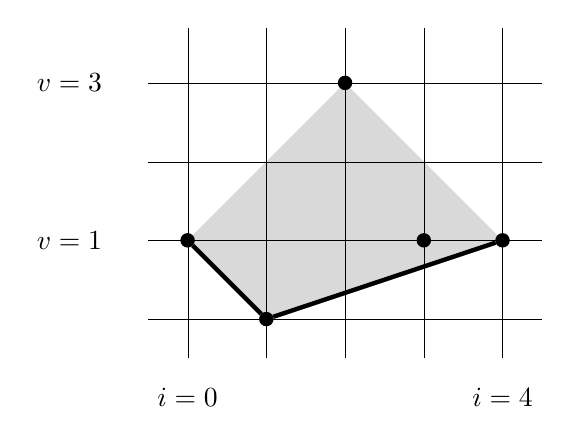
\begin{tikzpicture}[val/.style={circle, fill, draw, inner sep=1.7pt}]
		\fill[fill=gray!30] (0,1) -- (1,0) -- (4,1) -- (2,3) -- cycle;
		\node[val] (C0) at (0,1) {};
		\node[val] (C1) at (1,0) {};
		\node[val] (C2) at (2,3) {};
		\node[val] (C3) at (3,1) {};
		\node[val] (C4) at (4,1) {};
		\draw[ultra thick] (C0) -- (C1) -- (C4);
		\draw[step=1, line width=0.05pt] (-0.5, -0.5) grid (4.5, 3.7);
		\node at (0,-1) {$i=0$};  \node at (4,-1) {$i=4$};
		\node at (-1.5, 1) {$v=1$}; \node at (-1.5, 3) {$v=3$};
	\end{tikzpicture}\end{center}
	折线由斜率为 $-1$ 和 $\frac{1}{3}$ 的两线段构成.
\end{example}

\begin{theorem}\label{prop:Newton-polygon}
	符号如上, 则对每个 $s \in \R$,
	\[ \textbf{NP}(P)\; \text{中存在斜率为 $-s$ 的线段} \iff \exists \lambda \in \overline{K}, \; P(\lambda)=0 \; \wedge \; v(\lambda)=s. \]
	而且斜率 $-s$ 的线段投影在 $x$ 轴上的长度等于 $\overline{K}$ 中满足 $v(\lambda)=s$ 的根数 (计入重数).
\end{theorem}
\begin{proof}
	不妨假设 $a_0 a_n \neq 0$. 垂直平移 $\textbf{NP}(P)$ 后可进一步假设 $a_n = 1$.	列出 $P$ 的根 $\lambda_1, \ldots, \lambda_n \in \overline{K}$ (计入重数), 按赋值递增排列:
	\[\begin{tikzcd}[column sep=small, row sep=small]
		v(\lambda_1) = \cdots = v(\lambda_{t_1}) \arrow[phantom, r, "=" description] & v_1 \arrow[sloped, phantom, d, "<" description] & (t_1 \;\text{项}) \\
		v(\lambda_{t_1+1}) = \cdots = v(\lambda_{t_1 + t_2}) \arrow[phantom, r, "=" description] & v_2 \arrow[sloped, phantom, d, "<" description] & (t_2 \;\text{项}) \\
		\vdots & \vdots & \vdots
	\end{tikzcd}\]
	则 $v(a_n)=0$, 而且对 $0 \leq k < n$ 皆有
	\[ v(a_{n-k}) = v\left( \sum_{1 \leq i_1 < \cdots < i_k \leq n} \lambda_{i_1} \cdots \lambda_{i_k} \right) \geq \min_{i_1 < \cdots < i_k}\left\{ v(\lambda_{i_1}) + \cdots + v(\lambda_{i_k}) \right\}. \]
	于是当 $0 \leq k \leq t_1$ 时 $v(a_{n-k}) \geq k v_1$; 此外引理 \ref{prop:ultrametric} 蕴涵 $v(a_{n-t_1}) = t_1 v_1$, 因为右式的极小值恰好取在 $(i_1, \ldots, i_{t_1}) = (1, \ldots, t_1)$. 假如 $t_1=n$, 则这表明 $\textbf{NP}(P)$ 仅由一个斜率 $-v_1$ 的线段构成. 若 $t_1 < n$, 同理知
	\[ 0 \leq k \leq t_2 \implies v(a_{n-t_1-k}) \geq t_1 v_1 + k v_2, \quad v(a_{n-t_1-t_2}) = t_1 v_1 + t_2 v_2. \]
	准此要领, $\textbf{NP}(P)$ 从右至左由斜率为 $-v_1 > -v_2 > \cdots$ 的线段给出, 其在 $x$ 轴上的投影长依次为 $t_1, t_2, \ldots$ 如此等等.
\end{proof}

K.\ Hensel 的引理是分析学思想应用于代数学与数论的范例. 它的形式多样, 这里仅介绍其一.
\begin{theorem}[Hensel 引理]\label{prop:Hensel-lemma}\index{Hensel 引理}
	设 $K$ 对秩 $1$ 赋值 $v$ 完备, $P \in K^\circ[X]$. 若 $x_0 \in K^\circ$ 满足
	\[ v(P(x_0)) > 2v(P'(x_0)), \]
	其中 $P' \in K^\circ[X]$ 为 $P$ 的形式导数 (命题 \ref{prop:polynomial-derivation}), 则存在 $x \in K^\circ$ 使得 $P(x) = 0$ 并且
	\[ v(x - x_0) \geq v(P(x_0)) - v(P'(x_0)) > v(P'(x_0)). \]
	唯一性成立: 设 $x, x' \in K^\circ$ 为 $P$ 的根, 而且 $v(x - x_0)$ 和 $v(x' - x_0)$ 皆 $> v(P'(x_0))$, 则 $x=x'$.
\end{theorem}
\begin{proof}
	我们将构造 $K^\circ$ 中的序列 $x_0, x_1, \ldots$, 使得对所有 $i \geq 0$ 皆有
	\begin{equation}\label{eqn:Hensel-sequence} \begin{gathered}
		v(P(x_{i+1})) \geq v(P(x_i)) + \underbracket{v(P(x_0)) - 2 v(P'(x_0))}_{>0}, \\
		v(P'(x_{i+1})) = v(P'(x_0)), \\
		v(x_{i+1} - x_i) \geq v(P(x_i)) - v(P'(x_0)).
	\end{gathered}\end{equation}
	给定如上序列, 则 $v(P(x_i))$ 递增无上界, 命题 \ref{prop:ultrametric-series} 遂给出极限
	\[ x := \lim_{i \to \infty} x_i = x_0 + \sum_{i=0}^\infty (x_{i+1}-x_i)\; \in K^\circ, \qquad P(x)=0. \]
	此外 $v(P(x_i)) \geq v(P(x_0))$ 蕴涵 $v(x_{i+1} - x_i) \geq v(P(x_0)) - v(P'(x_0))$; 取极限得到 $v(x - x_0) \geq \inf_{i \geq 0} v(x_{i+1} - x_i) \geq v(P(x_0)) - v(P'(x_0))$. 所以 $x$ 具备所求之全部性质. 下一步是从 $x_0$ 出发, 递归地构造 $(x_i)_{i \geq 0}$.
	
	假设已构造满足 \eqref{eqn:Hensel-sequence} 的 $x_0, \ldots, x_i$, 其中 $i \geq 0$. 以下说明如何构造 $x_{i+1}$, 思路类似于 Newton 法. 兹引进新变元 $Y$, 置
	\[ P(X+Y) = P_0(X) + P_1(X) Y + P_2(X) Y^2 + \cdots, \quad P_k \in K^\circ[X]. \]
	易见 $P_0 = P$ 而 $P_1 = P'$. 条件蕴涵 $P_1(x_i) \neq 0$, 故可取 $t := -P(x_i)/P'(x_i)$, 它满足于
	\begin{align*}
		v(t) & = v(P(x_i)) - v(P'(x_i)) = v(P(x_i)) - v(P'(x_0)), \\
		2v(t) & = v(P(x_i)) + v(P(x_i)) - 2v(P'(x_0)) \\
		& \geq v(P(x_i)) + v(P(x_0)) - 2v(P'(x_0)) > 0.
	\end{align*}
	特别地 $v(t) > 0$, 从而 $x_{i+1} := x_i + t \;\in K^\circ$. 于是 $t$ 的选取导致
	\begin{gather*}
		P(x_{i+1}) = P(x_i + t) = \sum_{2 \leq k \leq \deg P} P_k(x_i) t^k, \\
		v(P(x_{i+1})) \geq 2v(t) \geq v(P(x_i)) + v(P(x_0)) - 2v(P'(x_0)), \\
		v(x_{i+1} - x_i) = v(t) = v(P(x_i)) - v(P'(x_0)).
	\end{gather*}
	
	同理, 由系数在 $K^\circ$ 上的展式 $P'(X+Y) = P'(X) + P''_1(X) Y + \cdots$ 可知
	\[ P'(x_{i+1}) - P'(x_i) \in  t \cdot K^\circ, \quad v(P'(x_{i+1}) - P'(x_i)) \geq v(t). \]
	然而 $v(t) \geq v(P(x_0)) - v(P'(x_0)) > v(P'(x_0))$, 又 $v(P'(x_i)) = v(P'(x_0))$, 引理 \ref{prop:ultrametric} 即刻给出 $v(P'(x_{i+1})) = v(P'(x_i))$. 如是造出满足 \eqref{eqn:Hensel-sequence} 的 $x_0, \ldots, x_{i+1}$.
	
	最后验证唯一性. 观察到 $x \in K^\circ$ 和 $v(x-x_0) > v(P'(x_0))$ 蕴涵 $P'(x) - P'(x_0) \in (x-x_0) K^\circ$ 的赋值大于 $v(P'(x_0))$, 于是引理 \ref{prop:ultrametric} 给出 $v(P'(x)) = v(P'(x_0))$. 现在考虑 $P$ 的相异根 $x, x' \in K^\circ$. 存在 $Q \in K^\circ[X]$ 使得 $P(X) = (X-x)(X-x') Q(X)$. 于是
	\begin{gather*}
		P'(x) = (x-x')Q(x), \\
		v(P'(x)) \geq v(x-x') \geq \min\left\{ v(x - x_0), v(x' - x_0) \right\}.
	\end{gather*}
	假若 $v(x-x_0), v(x'-x_0) > v(P'(x_0))$, 前述观察将导致 $v(P'(x_0)) \geq \cdots > v(P'(x_0))$, 矛盾.
\end{proof}

最常见的是 $v(P'(x_0))=0$ 的特例如下: 置 $\kappa := K^\circ/K^{\circ\circ}$ 为剩余类域, 以 $x \mapsto \bar{x}$ 表商同态 $K^\circ \twoheadrightarrow \kappa$. 任何 $Q \in K^\circ[X]$ 在 $\bmod \; K^{\circ\circ}$ 后可以在 $\bar{x}$ 处取值, 记为 $Q(\bar{x})$ 等等.
\begin{corollary}\label{prop:Hensel-lemma-unique}
	设 $K$ 对秩 $1$ 赋值 $v$ 完备, $P \in K^\circ[X]$. 若 $\bar{x}_0 \in \kappa$ 满足于 $P(\bar{x}_0) = 0$, $P'(\bar{x}_0) \neq 0$, 则存在唯一的 $x \in K^\circ$ 使得
	\[ \bar{x} = \bar{x}_0 \;\in \kappa, \qquad P(x)=0. \]
\end{corollary}
\begin{proof}
	任取 $x_0 \mapsto \bar{x}_0$, 条件变为 $v(P(x_0)) > 0$ 而 $v(P'(x_0))=0$. 代入定理 \ref{prop:Hensel-lemma}.
\end{proof}

在 $\kappa$ 中解方程比在 $K$ 中容易得多, 下面是一则关键例子. 对任意交换环 $R$ 和整数 $m \neq 0$, 定义乘法群 $\mu_m(R) := \left\{ x \in R^\times: x^m = 1 \right\}$.

\begin{example}[Teichmüller 代表元]\label{eg:Teichmuller-rep}
	设 $K$ 的剩余类域 $\kappa \simeq \F_q$, 其中 $q$ 是素数 $p$ 的幂. 给定非零整数 $m$, 我们有群同态
	\begin{align*}
		\mu_m(K) & \longrightarrow \mu_m(\kappa) \\
		x & \longmapsto x \bmod K^{\circ\circ}.
	\end{align*}
	当 $p \nmid m$ 时上式为同构: 考虑多项式 $P := X^m - 1 \in K^\circ[X]$. 每个 $\bar{x} \in \kappa^\times$ 皆满足 $P'(\bar{x}) = m\bar{x}^{m-1} \neq 0$, 于是推论 \ref{prop:Hensel-lemma-unique} 表明 $\mu_m(K) \rightiso \mu_m(\kappa)$. 对特例 $m = q-1$ 得到群同构
	\[ \mu_{q-1}(K) \stackrel{\sim}{\longrightarrow} \mu_{q-1}(\kappa) = \kappa^\times. \]
	对应于 $\bar{x} \in \kappa^\times$ 的 $x \in \mu_{q-1}(K)$ 称为 $\bar{x}$ 在 $K$ 中的 Teichmüller 代表元. 方便起见, 再定义 $0$ 的 Teichmüller 代表元为 $0 \in K$, 这样就得到乘法幺半群的嵌入 $\kappa \hookrightarrow K^\circ$.
\end{example}

\begin{theorem}[M.\ Krasner]\label{prop:Krasner-lemma}
	设 $K$ 对秩 $1$ 赋值 $v$ 完备. 取定可分闭包 $K^\mathrm{sep} \subset \overline{K}$ 并设 $x, y \in K^\mathrm{sep}$. 以 $x = x_1, \ldots, x_n \in K^\mathrm{sep}$ 表 $x$ 的极小多项式 $P_x \in K[X]$ 的所有根 (换言之: $x$ 的所有共轭元). 若
	\[ v(x-y) > v(x-x_i), \quad i=2, \ldots, n. \]
	则必有 $K(x) \subset K(y)$. 这里我们以推论 \ref{prop:valuation-ext-complete-alg} 将 $v$ 延拓到 $K^\mathrm{sep}$ 上.
\end{theorem}
\begin{proof}
	策略是证明 $x$ 被所有 $\sigma \in \Gal(K^\text{sep}|K(y))$ 固定, 继而从 Galois 对应 (定理 \ref{prop:infinite-Galois-corr}) 推出 $x \in K(y)$. 鉴于赋值延拓的唯一性, 对任意 $\sigma$ 如上皆有 $v \circ \sigma = v$, 从而
	\[ v(y-\sigma(x)) = v(\sigma(y-x)) = v(y-x) > v(x-x_i), \quad i=2, \ldots, n. \]
	于是乎
	\[ v(x-\sigma(x)) \geq \min\left\{ v(x-y), v(y-\sigma(x)) \right\}  > v(x-x_i), \quad i=2, \ldots, n. \]
	因为存在 $1 \leq j \leq n$ 使得 $\sigma(x) = x_j$; 上述不等式遂导致 $j=1$, $\sigma(x)=x$.
\end{proof}

\begin{corollary}\label{prop:complete-alg-closed}
	设 $|\cdot|$ 是可分闭域 (或代数闭域) $K$ 上的绝对值, 则相应的完备化 $\hat{K}$ 也是可分闭域 (或代数闭域).
\end{corollary}
回忆到 $K$ 可分闭意谓它在 $\overline{K}$ 中的可分闭包等于自身, 当 $\text{char}(K)=0$ 时这等价于代数闭.

\begin{proof}
	若 $|\cdot|$ 是 Archimedes 绝对值, 则定理 \ref{prop:archimedean-complete-field} 蕴涵 $\hat{K}=\R$ 或 $\CC$; 前一情形将导致 $\Q \subset K \subset \R$, 不可能代数闭. 因此以下可假定 $|\cdot|$ 非 Archimedes, 对应于 $K$ 的一个秩 $1$ 赋值. 对于可分闭域情形, 设 $x \in \hat{K}^{\text{sep}}$, 由于 $K$ 在 $\hat{K}$ 中稠密, 可取首一的 $P \in K[X]$ 使其系数足够接近 $P_x$, 于是 $|P(x)|=|P(x)-P_x(x)|$ 亦可取到任意小. 考察多项式的判别式 (例 \ref{eg:polynomial-discriminant}) 知 $P$ 和 $P_x$ 一样无重根, 故 $P$ 分裂成一次因子, 并且存在根 $y \in K$ 使得 $|y-x|$ 充分小. 从定理 \ref{prop:Krasner-lemma} 立得 $\hat{K}(x) \subset \hat{K}(y) = \hat{K}$.
	
	对于代数闭域情形, 无妨设 $\text{char}(K) = p > 0$. 设 $x \in \overline{\hat{K}}$, 其在 $\hat{K}$ 上的极小多项式写作 $P_x(X) = P_x^\flat(X^{p^m})$ 之形, 其中 $P_x^\flat$ 无重根. 因此 $y := x^{p^m} \in \hat{K}^{\text{sep}}$; 由上一步知 $\hat{K}^{\text{sep}} = \hat{K}$, 故可取 $K$ 中点列 $y_1, y_2, \ldots$ 使得 $|y_k - y| \to 0$. 易见 $\left| y_k^{p^{-m}} - y^{p^{-m}} \right| \to 0$, 于是 $x = y^{p^{-m}} \in \hat{K}$. 明所欲证.
\end{proof}

\section{Witt 向量}\label{sec:Witt-vector}
本节取定素数 $p$.

我们先回忆 $p$-进整数环 $\Z_p$ 的结构. 由于 $\Z_p/p\Z_p$ 可等同于 $\F_p$, 可选定某一映射 $\tau: \F_p \to \Z_p$ 使得 $\tau(x) \equiv x \pmod {p\Z_p}$, 称 $\tau(x)$ 为 $x$ 的一个提升. 设 $\tilde{x} \in \Z_p$, 记它在 $\F_p$ 中的像为 $x$, 则 存在 $\tilde{x}_1 \in \Z_p$ 使得 $\tilde{x} = \tau(x) + p \tilde{x}_1$; 因 $p$ 非零因子, $\tilde{x}_1$ 唯一. 重复操作可得 $\tilde{x}_1 = \tau(x_1) + p\tilde{x}_2$ 等等, 于是得到 $\F_p$ 中唯一确定的序列 $x_0, x_1, \ldots$, 使得 $n \geq 0$ 时
\[ \tilde{x} = \tau(x_0) + \tau(x_1) p + \cdots + \tau(x_n) p^n + \tilde{x}_{n+1} p^{n+1}, \quad \tilde{x}_{n+1} \in \Z_p. \]
无穷级数 $\sum_{n=0}^\infty \tau(x_n) p^n$ 在 $\Z_p$ 中收敛到 $\tilde{x}$. 反之, 根据命题 \ref{prop:ultrametric-series}, 任意数列 $\left( x_n \in \F_p \right)_{n \geq 0}$ 确定了 $\tilde{x} := \sum_{n=0}^\infty \tau(x_n) p^n \in \Z_p$. 综上得出集合的双射
\begin{align*}
	\prod_{n \geq 0} \F_p & \stackrel{1:1}{\longrightarrow} \Z_p \\
	(x_n)_{n \geq 0} & \longmapsto \sum_{n=0}^\infty \tau(x_n) p^n.
\end{align*}
这般描述简则简矣, 问题在于
\begin{compactitem}
	\item 双射与提升 $x \mapsto \tau(x)$ 的选取有关, 对之是否有一个典范的, 方便的取法?
	\item $\Z_p$ 的环结构如何体现在 $\prod_{n \geq 0} \F_p$ 上?
\end{compactitem}
对于第一个问题, 例 \ref{eg:Teichmuller-rep} 给出了一个标准的 $\tau: \F_p \to \Z_p$, 它同时还是乘法幺半群的同态. 要完满解答第二个问题, 我们宜将视野放广.

\begin{definition}\index{daishu!完全}
	设 $\kappa$ 为交换 $\F_p$-代数. 若 $\Frob_p: x \mapsto x^p$ 是 $\kappa$ 的自同构, 则称 $\kappa$ 为\emph{完全}的.
\end{definition}
这是域的情形的自然延伸, 见定理 \ref{prop:perfect-field-char}. 定义 \ref{def:Frob-aut} 也涉及了类似的映射.

\begin{definition}\label{def:p-ring} \index{yangepihuan@严格 $p$-环 (strict $p$-ring)}
	设 $A$ 为交换环, 并给定理想降链 $\mathfrak{a}_1 \supset \mathfrak{a}_2 \supset \cdots$ 使得
	\begin{compactitem}
		\item 相应的拓扑使 $A$ 成为完备 Hausdorff 拓扑环 (见注记 \ref{rem:ring-completion}), 亦即 $A \rightiso \varprojlim_n A/\mathfrak{a}_n$;
		\item 对每个 $n, m$ 皆有 $\mathfrak{a}_n \mathfrak{a}_m \subset \mathfrak{a}_{n+m}$;
		\item $p \in \mathfrak{a}_1$ 并且剩余环 $\kappa := A/\mathfrak{a}_1$ 是完全的.
	\end{compactitem}
	我们称 $A$ 对这些资料构成 $p$-环. 如进一步要求 $p$ 在 $A$ 中非零因子, 而且 $\mathfrak{a}_n = p^n A$, 则称 $A$ 为严格 $p$-环.
\end{definition}
例如 $\Z_p$ 是严格 $p$-环, 而 $\F_p$-代数 $\F_p \llbracket t \rrbracket$ 对 $\mathfrak{a}_n := (t^n)$ 构成 $p$-环, 但显然不严格.

\begin{lemma}\label{prop:aux-p-power}
	设交换环 $A$ 具有理想降链 $\mathfrak{a}_1 \supset \mathfrak{a}_2 \supset \cdots$ 使得 $\mathfrak{a}_n \mathfrak{a}_m \subset \mathfrak{a}_{n+m}$ 而 $p \in \mathfrak{a}_1$, 则对任意 $a,b \in A$ 皆有
	\[ a \equiv b \pmod{\mathfrak{a}_m} \implies a^{p^n} \equiv b^{p^n} \pmod{\mathfrak{a}_{m+n}}. \]
\end{lemma}
此结果可谓是本节一切论证的枢纽, 实用中常取 $\mathfrak{a}_n = p^n A$ 的情形.
\begin{proof}
	易化约到 $n=1$ 的情形. 其次置 $P(X,Y) := \frac{X^p-Y^p}{X-Y} \in \Z[X,Y]$, 条件蕴涵 $P(a,b) \equiv P(a,a) \equiv pa^{p-1} \pmod{\mathfrak{a}_m}$, 于是 $a^p - b^p = (a-b) P(a,b)$ 属于 $\mathfrak{a}_m (pA + \mathfrak{a}_m) \subset \mathfrak{a}_{m+1}$. 证毕.
\end{proof}

\begin{proposition}\label{prop:Teichmuller-lift}\index{Teichmüller 提升}
	设 $A$ 为 $p$-环, $\kappa := A/\mathfrak{a}_1$, 则存在唯一的映射 $\tau: \kappa \to A$ 使得
	\begin{compactitem}
		\item $\tau(x)$ 在 $\kappa$ 中的像为 $x$;
		\item $\tau$ 满足乘性: $\tau(1)=1$, $\tau(xy)=\tau(x)\tau(y)$.
	\end{compactitem}
	称 $\tau$ 为 Teichmüller 提升. 若 $A$ 是 $\F_p$-代数, 则 $\tau$ 也满足加性 $\tau(x+y)=\tau(x)+\tau(y)$.
\end{proposition}
\begin{proof}
	由于 $\kappa$ 是完全的, 对 $x \in \kappa$ 和任意 $n \geq 0$ 存在唯一的 $p^n$-次根 $x^{p^{-n}} \in \kappa$, 对之任取 $A$ 中原像 $\left[ x^{p^{-n}} \right]$. 我们希望定义
	\[ \tau(x) := \lim_{n \to \infty} \left[ x^{p^{-n}} \right]^{p^n}. \]
	当 $n \geq m$ 时 $\left[ x^{p^{-n}} \right]^{p^{n-m}}$ 是 $x^{p^{-m}}$ 的一个原像, 不妨就记作 $\left[ x^{p^{-m}} \right]$. 引理 \ref{prop:aux-p-power} 蕴涵
	\[ \left[ x^{p^{-n}} \right]^{p^n} = \left[ x^{p^{-m}} \right]^{p^m} \;\text{在}\; A/\mathfrak{a}_{m+1}\; \text{中的像仅依赖于}\; x^{p^{-m}} \in \kappa \]
	因为 $A$ 完备, 这说明定义 $\tau$ 的极限确实存在, 而且仅和 $x$ 有关. 显然 $\tau(x) \equiv x \pmod{\mathfrak{a}_1}$.

	性质 $(xy)^{p^{-n}} = x^{p^{-n}} y^{p^{-n}}$ 蕴涵 $\tau$ 的乘性, 而且任意乘性提升 $\tau': \kappa \to A$ 都满足 $\tau'( x^{p^{-n}})^{p^n} = \tau'(x)$, 在先前论证中取 $\left[ \cdots \right] = \tau'(\cdots)$ 便导出唯一性 $\tau=\tau'$. 最后, 当 $A$ 是 $\F_p$-代数时, 以上构造和 $A$ 中公式 $\tilde{x}^p + \tilde{y}^p = (\tilde{x}+\tilde{y})^p$ 确保 $\tau$ 的加性.
\end{proof}

令 $A$ 为严格 $p$-环, $\kappa := A/pA$. 现在可以照搬本节开头处理 $\Z_p$ 的方法, 得到典范的集合双射
\begin{equation}\label{eqn:Witt-bijection}\begin{aligned}
	\prod_{n \geq 0} \kappa & \stackrel{1:1}{\longrightarrow} A \\
	(x_n)_{n \geq 0} & \longmapsto \sum_{n=0}^\infty \tau\left( x_n^{p^{-n}} \right) p^n.
\end{aligned}\end{equation}
环 $A$ 的零元和幺元显然对应于 $(0,0,\ldots)$ 和 $(1, 0, \ldots)$. 注意到当 $\kappa = \F_p$ 时恒有 $x^{p^{-n}} = x$. 取 $x^{p^{-n}}$ 的妙用将在后续证明中体现.

我们欲探讨 $A$ 的环结构如何拉回到 $\prod_{n \geq 0} \kappa$ 上, 相应的环将另外记为 $\WittV(\kappa)$, 以区别于直积. 兹以加法为例, 置
\[ \sum_{n \geq 0} \tau\left( S_n(x_0, \ldots, y_0, \ldots)^{p^{-n}} \right) p^n = \sum_{n \geq 0} \tau(x_n^{p^{-n}}) p^n + \sum_{n \geq 0} \tau(y_n^{p^{-n}}) p^n, \]
如何描述 $S_n$? 首先对上述等式两边同模 $pA$, 可知 $S_0 = x_0 + y_0 \in \kappa$. 为了描述 $S_1$, 必须考察
\[ \tau(x_0 + y_0) + \tau( S_1^{p^{-1}} )p \equiv \tau(x_0) + \tau(y_0) + \left( \tau(x_1^{p^{-1}}) + \tau(y_1^{p^{-1}}) \right)p \pmod{p^2 A}. \]
如何确定 $\tau(x_0) + \tau(y_0) - \tau(x_0+y_0)\; \bmod p^2 A$? 诀窍在于回忆命题 \ref{prop:Teichmuller-lift} 之证明
\begin{equation}\label{eqn:Teich-lifting-power}
	\tau(z) \equiv \left[ z^{p^{-n}} \right]^{p^n} \pmod{ p^{n+1} A}, \quad z \in \kappa,
\end{equation}
其中 $[\cdots]$ 是任意原像. 引理 \ref{prop:aux-p-power} 给出 $[x^{1/p} + y^{1/p}]^p \equiv \left( [x^{1/p}] + [y^{1/p}] \right)^p \pmod {p^2 A}$. 因为 $p \in A$ 非零因子, 从模 $p^2 A$ 的同余式得出
\begin{align*}
	S_1^{p^{-1}} & = x_1^{1/p} + y_1^{1/p} + \frac{1}{p} \left( \left[ x_0^{1/p} \right]^p + \left[ y_0^{1/p} \right]^p - \left[ x_0^{1/p} + y_0^{1/p} \right]^p \right) \bmod pA \\
	& = x_1^{1/p} + y_1^{1/p} - \sum_{0 < k < p} \frac{1}{p} \binom{p}{k} \left[ x_0^{1/p} \right]^k \left[ y_0^{1/p} \right]^{p-k} \bmod pA.
\end{align*}
对两边应用 $z \mapsto z^p$ 和 $\left[ z^{1/p} \right]^p \equiv z \pmod {pA}$ 可得
\[ S_1 = x_1 + y_1 - \sum_{0 < k < p} \frac{1}{p} \binom{p}{k} x_0^k y_0^{p-k}. \]
高阶项 $S_2, S_3, \ldots$ 的面貌比较复杂, 但算法是明确的. 由此不难察觉
\begin{compactitem}
	\item 环 $A$ 的加法和乘法反映在 $\WittV(\kappa)$ 上, 由一族多项式 $S_n$, $P_n$ 按分量给出;
	\item 这族多项式的形式和 $A$ 或 $\kappa$ 无关, 并且可以按递归方式写作整系数多项式.
\end{compactitem}
这就提示了严格 $p$-环的结构应该具备某种泛性. E.\ Witt 的工作 \cite{Witt37} 出色地解决了这些问题. 然而为了构造 $S_n, P_n$, 我们势必要考虑分量 $x_i$ 取值在一般交换环 $R$ 中的情形, 并探讨相对应的 Witt 环 $\WittV(R)$; 这般迂回不仅必要, 而且正是 Witt 工作的精华所在.

以下将借鉴 \cite[\S 1]{Hess15} 的处理方式, 差别在于该文一次涵摄了所有的素数 $p$, 获得的环称为大 Witt 环.

\begin{definition}
	设 $R$ 为交换环, 定义 $\WittV(R) := \prod_{i \geq 0} R$, 并对每个 $n \geq 0$ 定义映射
	\begin{align*}
		w_n: \WittV(R) & \longrightarrow R \\
		x = (x_j)_{j \geq 0} & \longmapsto w_n(x_0, \ldots, x_n) = \sum_{i=0}^n x_i^{p^{n-i}} p^i.
	\end{align*}
	进一步定义 $w: \WittV(R) \to \prod_{n \geq 0} R$ 为 $w(x) := (w_0(x), w_1(x), w_2(x), \ldots)$.
\end{definition}
传统上称 $w_n(x)$ 为 $x$ 的第 $n$ 个幻影分量 (德文: \textit{die Geisterkomponente}), 因为在我们的原始问题中 $R=\kappa$ 总是 $\F_p$-代数, 这时 $w_n(x)$ 坍缩为 $x_0^{p^n}$, 然而解开 $\WittV(\kappa)$ 秘密的钥匙正是剩下的``幻影''. 此外尚有几点观察:
\begin{compactitem}
	\item 对于任意的交换环同态 $\phi: R \to S$, 相应地有映射 $\WittV(\phi): \WittV(R) \to \WittV(S)$, 它映 $(x_i)_i$ 为 $(\phi(x_i))_i$.
	\item 映射 $w$ 的值域 $\prod_{i \geq 0} R$ 具有直积的环结构 (定义 \ref{def:ring-direct-product}), 亦即逐分量地进行环运算.
	\item 称 $R$ 是 $p$-无挠的, 如果 $pr =0 \iff r=0$ 对所有 $r \in R$ 恒成立. 在 $p$-无挠的条件下, 从 $w_0, \ldots, w_n$ 可以逐步反解 $x_0, \ldots, x_n$, 故此时 $w$ 是单射. \index{$p$-无挠 ($p$-torsion free)}
\end{compactitem}

下面的任务是赋予 $\WittV(R)$ 自然的环结构; 由于 Witt 环 $\WittV(R)$ 作为集合等于 $R \times R \times \cdots$, 前人称 $\WittV(R)$ 的元素为 Witt 向量\index{Witt 向量}. 我们需要一个方便的引理.
\begin{lemma}[B.\ Dwork]\label{prop:Dwork-Witt}
	假定存在环同态 $\phi_p: R \to R$ 使得 $\phi_p(r) \equiv r^p \pmod {pR}$, 则 $w$ 的像等于
	\[ \left\{ (r_n)_{n \geq 0} \in \prod_{n \geq 0} R : \quad \forall n \geq 1, \; r_n \equiv \phi_p(r_{n-1}) \pmod {p^n R}  \right\}. \]
\end{lemma}
\begin{proof}
	由于 $\phi_p$ 是环同态, 当 $n \geq 1$ 时根据引理 \ref{prop:aux-p-power} 得到
	\[ \phi_p(w_{n-1}(x)) = \sum_{i < n} \phi_p(x_i)^{p^{n-1-i}} p^i \equiv \sum_{i < n} x_i^{p^{n-i}} p^i \pmod {p^n R}. \]
	故确有 $w_n(x) \equiv \phi_p(w_{n-1}(x)) \pmod {p^n R}$. 反之给定一列 $r_0, r_1, \ldots \in R$ 满足于 $r_n \equiv \phi_p(r_{n-1}) \pmod {p^n R}$, 我们递归地构作 $x_0 := r_0, \ldots, x_{n-1} \in R$ 并假设 $i < n \implies w_i((x_0, \ldots, x_i)) = r_i$, 那么前段论证给出
	\[ r_n - \sum_{i < n} x_i^{p^{n-i}} p^i \equiv r_n - \phi_p(w_{n-1}(x)) \equiv 0 \pmod {p^n R}, \]
	故存在 $x_n \in R$ 使得 $r_n = \sum_{i<n} x_i^{p^{n-i}} p^i + x_n p^n$, 亦即 $r_n = w_n(x_0, \ldots, x_n)$.
\end{proof}
于是在引理的条件下立见 $\Image(w)$ 为 $\prod_{i \geq 0} R$ 的子环.

\begin{theorem}\label{prop:Witt-ring}\index{Witt 环}
	在所有 $\WittV(R)$ 上存在唯一的一族交换环结构, 使得 $w: \WittV(R) \to \prod_{n \geq 0} R$ 为环同态, $(0, 0, \ldots)$ 为零元, $(1, 0, \ldots)$ 为幺元, 而且:
	\begin{itemize}
		\item 对每个环同态 $\phi: R \to S$ 下图皆在 $\cate{CRing}$ 中交换
		\[\begin{tikzcd}
		\WittV(R) \arrow[d, "w"'] \arrow[r, "\WittV(\phi)"] & \WittV(S) \arrow[d, "w"] \\
		\prod_{n \geq 0} R \arrow[r, "\prod_n \phi"'] & \prod_{n \geq 0} S
		\end{tikzcd}\]
		\item 存在唯一确定的多项式族 $S_n \in \Z[X_0, \ldots, Y_0, \ldots]$, $P_n \in \Z[X_0, \ldots, Y_0, \ldots]$ 和 $M_n \in \Z[X_0, \ldots, X_n]$ 使得 $\WittV(R)$ 的环结构由
		\begin{align*}
			(x_n)_{n \geq 0} + (y_n)_{n \geq 0} & = (S_n(x_0, \ldots, x_n, y_0, \ldots, y_n))_{n \geq 0}, \\
			(x_n)_{n \geq 0} \cdot (y_n)_{n \geq 0} & = (P_n(x_0, \ldots, x_n, y_0, \ldots, y_n))_{n \geq 0}, \\
			-(x_n)_{n \geq 0} & = (M_n(x_0, \ldots, x_n))_{n \geq 0}
		\end{align*}
		所确定, 这些多项式与 $R$ 无关.
	\end{itemize}
	因此 $\WittV(\cdot)$ 给出从交换环范畴 $\cate{CRing}$ 到自身的函子.
\end{theorem}
\begin{proof}
	给定 $(x_i)_i, (y_i)_i \in \WittV(R)$, 为了定义其间自然的 (即对 $R$ 具函子性) 环运算, 我们先取 $x_i := X_i$, $y_i := Y_i$ 为自由变元, 而 $R := \Z[X_0, \ldots, Y_0, \ldots]$. 根据多项式环的泛性质, 存在自同态 $\phi_p: R \to R$ 使得
	\[ \phi_p(X_n) = X_n^p, \quad \phi_p(Y_n) = Y_n^p, \]
	配合 Fermat 小定理 (注记 \ref{rem:Fermat-little}) 可知 $\forall r \; \phi_p(r) = r^p \pmod{pR}$. 引理 \ref{prop:Dwork-Witt} 确保环 $\prod_{n \geq 0} R$ 的元素
	\[ w(x) + w(y), \quad w(x)w(y), \quad -w(x) \]
	仍落在 $\Image(w)$ 中. 因 $R$ 为 $p$-无挠, 它们对 $w$ 的原像皆唯一, 分别记为 $(S_i)_i, (P_i)_i, (M_i)_i$ (处理 $M_i$ 时改用环 $\Z[X_0, X_1, \ldots]$); 又由引理的证明可知 $S_i, P_i, M_i$ 仅涉及变元 $X_0, \ldots, X_i$ 和 $Y_0, \ldots, Y_i$. 我们断言对一般的 $R$, 这些整系数多项式使 $\WittV(R)$ 成交换环:
	\begin{gather*}
		(x_i)_i + (y_i)_i = (S_i(x,y))_i, \quad (x_i)_i (y_i)_i = (P_i(x,y))_i, \quad  -(x_i)_i = (M_i(x))_i, \\
		0_{\WittV(R)} = (0,0, \ldots), \quad 1_{\WittV(R)} = (1,0,\ldots).
	\end{gather*}
	兹举加法为例, 利用从 $\Z[X_0, \ldots, Y_0, \ldots]$ 到 $R$ 的同态
	$\begin{tikzcd}[row sep=0pt, column sep=small] X_i \arrow[mapsto, r] & x_i \\ Y_i \arrow[mapsto, r] & y_i \end{tikzcd}$,
	以上对自由变元的定义说明图表
	\[\begin{tikzcd}
		\WittV(R) \times \WittV(R) \arrow[d, "{(S_i)_i}"'] \arrow[r, "{(w,w)}"] & \prod_{i \geq 0} R  \times \prod_{i \geq 0} R \arrow[d, "+"] \\
		\WittV(R) \arrow[r, "w"'] & \prod_{i \geq 0} R
	\end{tikzcd}\]
	交换. 当 $R$ 为 $p$-无挠时 $w$ 为单射, 而且 $w(0_{\WittV(R)}) = (0, \ldots, 0)$ 故交换律, 结合律和零元等性质继承自 $\prod_{i \geq 0} R$. 对于一般的 $R$, 取定一族生成元 $\mathcal{X} \subset R$ 并构作多项式环 $R' := \Z[\mathcal{X}]$; 相应地有满射 $R' \twoheadrightarrow R$ 和 $\WittV(R') \twoheadrightarrow \WittV(R)$. 由于 $R'$ 为 $p$-无挠, $\WittV(R)$ 的环论公理仍可化约到 $\WittV(R')$ 上检验.
	
	同理可证对任意环同态 $\phi: R \to S$, 映射 $\WittV(\phi): \WittV(R) \to \WittV(S)$ 是环同态. 这套论证也表明了所求环结构的唯一性.
\end{proof}

由于 $S_n$, $P_n$ 和 $M_n$ 只涉及变元 $X_0, \ldots, X_n$ 和 $Y_0, \ldots, Y_n$, 可定义截断的 Witt 环 \index[sym1]{Witt@$\WittV(R)$, $\WittV_n(R)$}
\[ \WittV_n(R)  := \left\{ (x_0, \ldots, x_{n-1}) : x_i \in R \right\}. \]
它依然具备映射 $w_i: \WittV_n(R) \to R$ ($0 \leq i < n$), 并且有自然的环同态 $\WittV(\cdot) \to \WittV_n(\cdot)$ 和 $\WittV_{n+1}(\cdot) \to \WittV_n(\cdot)$ (即``截断'') 等等. 请读者验证环 $\WittV_1(R)$ 实际就是 $R$.

Witt 环上还有如下几种简单然而极重要的运算.
\begin{enumerate}
	\item 移位 (德文: \textit{die Verschiebung}) $V: \WittV(R) \to \WittV(R)$, 映 $(x_0, x_1, \ldots)$ 为 $(0, x_0, x_1, \ldots)$. 显然 $V$ 满足函子性: 对于任意环同态 $\phi: R \to S$ 皆有 $V \circ \WittV(\phi) = \WittV(\phi) \circ V$. 下面说明 $V$ 实则是加法群的同态: 易见下图交换
		\[\begin{tikzcd}
			\WittV(R) \arrow[r, "w"] \arrow[d, "V"'] & \prod_{n \geq 0} R \arrow[d, "{V^w}"] & (y_i)_{i \geq 0} \arrow[phantom, l, "\ni" description] \arrow[mapsto, d] \\
			\WittV(R) \arrow[r, "w"'] & \prod_{n \geq 0} R & (0, py_0, py_1, \ldots) \arrow[phantom, l, "\ni" description]
		\end{tikzcd}\]
		显然 $V^w$ 是加法群的同态; 当 $R$ 为 $p$-无挠时 $w$ 为单同态, 故 $V$ 亦满足加性; 对于一般的 $R$ 可按定理 \ref{prop:Witt-ring} 的证明处理.
	\item Frobenius 同态 $F: \WittV(R) \to \WittV(R)$. 它被刻画为对 $R$ 具函子性并使下图交换的一族同态
		\[\begin{tikzcd}
			\WittV(R) \arrow[r, "w"] \arrow[d, "F"'] & \prod_{n \geq 0} R \arrow[d, "{F^w}"] & (y_i)_{i \geq 0} \arrow[phantom, l, "\ni" description] \arrow[mapsto, d] \\
			\WittV(R) \arrow[r, "w"'] & \prod_{n \geq 0} R & (y_1, y_2, \ldots) \arrow[phantom, l, "\ni" description]
		\end{tikzcd} \]
		其验证同于定理 \ref{prop:Witt-ring} 的证明: 我们先考虑以自由变元为分量的元素 $(X_i)_{i \geq 0} \in \WittV(\Z[X_0, \ldots])$, 并注意到环 $\Z[X_0, \ldots]$ 带有自同态 $\phi_p: X_i \mapsto X_i^p$ 满足 $\phi_p(x) \equiv x^p \pmod p$. 应用引理 \ref{prop:Dwork-Witt} 以说明 $F^w(w(X_0, X_1, \ldots)) \in \Image(w)$, 其唯一的原像记为 $(F_i(X_0, X_1, \ldots))_{i \geq 0} \in \WittV(\Z[X_0, \ldots])$. 这就为任意环 $R$ 定义了 $F(x_0, x_1, \ldots) = (F_i(x_0, x_1, \ldots))_{i \geq 0}$. 要证明 $F$ 为环同态, 只须注意到 $F^w$ 也是环同态, 并重复定理 \ref{prop:Witt-ring} 证明的技巧. 同理可证函子性.
	\item Teichmüller 提升 $\tau: R \to \WittV(R)$, 它映 $x$ 为 $(x,0,0, \ldots)$. 此映射显然也对 $R$ 满足函子性, 并且有交换图表
		\[\begin{tikzcd}[column sep=tiny]
			& R \arrow[ld, "\tau"'] \arrow[rd, "\tau^w"] & x \arrow[phantom, l, "\ni" description] \arrow[mapsto, rd] & \\
			\WittV(R) \arrow[rr, "w"'] & & \prod_{n \geq 0} R & (x^{p^i})_{i \geq 0} \arrow[phantom, l, "\ni" description]
		\end{tikzcd}\]
		显然 $\tau^w$ 是乘法幺半群的同态, 运用上述论证化约到 $p$-无挠情形, 可知 $\tau$ 亦满足乘性 $\tau(xy)=\tau(x)\tau(y)$, 而且 $\tau(1) = (1,0, \ldots) = 1_{\WittV(R)}$.
\end{enumerate}

此外 $\Ker[ \WittV(\cdot) \twoheadrightarrow \WittV_n(\cdot)] = \Image(V^n)$, 特别地 $\Image(V^n)$ 是理想; 而且映射 $V$ 同样可以定义在截断版本 $\WittV_n(\cdot)$ 上, 给出加法群的短正合列
\begin{equation}\label{eqn:Witt-V}\begin{tikzcd}[row sep=tiny]
	0 \arrow[r] & \WittV_n(\cdot) \arrow[r, "V^r"] & \WittV_{n+r}(\cdot) \arrow[r, "(\text{截断})^n"] & \WittV_r(\cdot) \arrow[r] & 0 \\
	& (x_0, \ldots, x_{n-1}) \arrow[mapsto, r] & (0, \ldots, 0, x_0, \ldots, x_{n-1}) & & \\
	& & (y_0, \ldots, y_{n+r-1}) \arrow[mapsto, r] & (y_0, \ldots, y_{r-1}) &
\end{tikzcd}\end{equation}
综之, 无论 $\WittV(R)$, $\WittV_n(R)$ 还是它们之间的同态和运算 $V$, $F$ 等, 对环 $R$ 都具函子性. 如只看 $\WittV(R)$, $\WittV_n(R)$ 的加法群结构, 则我们造出的实则是一族定义 \ref{def:group-functor} 下的群函子, 连同其间的态射 $\WittV(\cdot) \to \WittV_n(\cdot)$ 和 $V$, $F$ 等等. 这点对于算术代数几何中的应用至关紧要, 它们是 Dieudonné 模理论的起点.

\begin{lemma}\label{prop:Frob-Witt-char-p}
	记 $(x_i)_{i \geq 0} \in \WittV(R)$ 在 $F$ 下的像为 $(F(x)_i)_{i \geq 0}$, 则对每个 $n$ 都有 $F(x)_n \equiv x_n^p \pmod{pR}$.
\end{lemma}
\begin{proof}
	处理 $x_i = X_i$ 是自由变元而 $R=\Z[X_0, \ldots]$ 的情形即可. 定义 $F_n \in \Z[X_0, \ldots]$ 的条件是当 $n \geq 0$ 时 $w_n(F_0, F_1, \ldots) = w_{n+1}(X_0, X_1, \ldots)$, 亦即
	\[ \sum_{i=0}^n F_i^{p^{n-i}} p^i = \sum_{i=0}^{n+1} X_i^{p^{n+1-i}} p^i. \]
	当 $n=0$ 时这表明 $F_0 = X_0^p + pX_1 \equiv X_0^p \pmod {pR}$. 今假设 $i < n \implies F_i \equiv X_i^p \pmod{pR}$, 上式变为
	\[ F_n p^n = X_{n+1} p^{n+1} + X_n^p p^n + \sum_{i<n} \left( X_i^{p^{n+1-i}} - F_i^{p^{n-i}} \right) p^i. \]
	引理 \ref{prop:aux-p-power} 及递归假设蕴涵 $i < n \implies F_i^{p^{n-i}} \equiv X_i^{p^{n+1-i}} \pmod{p^{n+1-i} R}$, 故
	\[ F_n p^n \equiv X_n^p p^n \pmod{p^{n+1} R}. \]
	由于 $R$ 是 $p$-无挠的, 因之有 $F_n \equiv X_n^p \pmod{pR}$. 证毕.
\end{proof}

\begin{proposition}\label{prop:FV-VF}
	对任意交换环 $R$, 上述映射满足关系式
	\begin{align*}
		F V(x) & = px, \\
		V (F(x) y) & = x V(y);
	\end{align*}
	当 $R$ 是 $\F_p$-代数时, 进一步有
	\begin{gather*}
		F\left((x_i)_{i \geq 0} \right) = (x_i^p)_{i \geq 0}, \\
		F V (x) = V F (x) = px.
	\end{gather*}
\end{proposition}
\begin{proof}
	对于前两条等式, 只消在 $\prod_{n \geq 0} R$ 中对 $F^w$ 和 $V^w$ 验证相应的关系. 当$R$ 是 $\F_p$-代数时, 引理 \ref{prop:Frob-Witt-char-p} 蕴涵 $F(x_0, x_1, \ldots) = (x_0^p, x_1^p, \ldots)$; 此时当然有 $VF(x) = FV(x) = (0, x_0^p, x_1^p, \ldots)$, 证毕.
\end{proof}

等式 $FV = p$ 导致 $F\left(\Image(V^{n+1})\right) = p \Image(V^n)$, 所以 $F$ 诱导出截断 Witt 环的同态 $W_{n+1}(R) \xrightarrow{F} W_n(R)$. 综之, 我们有三道自然映射:
\[\begin{tikzcd}[column sep=large]
	W_n(R) \arrow[r, "V" description] & W_{n+1}(R) \arrow[l, bend right=20, "F"'] \arrow[l, bend left=20, "\text{截断}"]
\end{tikzcd}, \quad n \in \Z_{\geq 1}. \]
对于完全 $\F_p$-代数, $W(\cdot)$ 和 $W_n(\cdot)$ 的结构更为清晰.

\begin{lemma}\label{prop:Witt-p-strict}
	设 $\kappa$ 为完全 $\F_p$-代数, 则 $\WittV(\kappa)$ 成为严格 $p$-环, 并具有一族自然同构 $\WittV(\kappa)/p^n \WittV(\kappa) \rightiso \WittV_n(\kappa)$, 其中 $n \geq 1$. 特别地, 我们有自然同构 $\WittV(\kappa)/p\WittV(\kappa) \rightiso \kappa$.
\end{lemma}
\begin{proof}
	由于 $\kappa$ 是完全 $\F_p$-代数, 命题 \ref{prop:FV-VF} 给出 $VF = p = FV$ 及 $F \WittV(\kappa) = \WittV(\kappa)$, 故
	\[ p^n \WittV(\kappa) = V^n F^n \WittV(\kappa) = V^n \WittV(\kappa) = \Ker \left[ \WittV(\kappa) \to \WittV_n(\kappa) \right], \]
	因之 $\WittV(\kappa)/p^n \WittV(\kappa) \rightiso \WittV_n(\kappa)$, 特别地 $\WittV(\kappa)/p\WittV(\kappa) \rightiso \kappa$. 此外易见下图交换
	\[\begin{tikzcd}
		\WittV(\kappa)/p^{n+1} \WittV(\kappa) \arrow[r, "\sim"] \arrow[d] & \WittV_{n+1}(\kappa) \arrow[d] \\
		\WittV(\kappa)/p^n \WittV(\kappa) \arrow[r, "\sim"'] & \WittV_n(\kappa)
	\end{tikzcd}\]
	而 $\WittV(\kappa)$ 按构造可等同于 $\varprojlim_n \WittV_n(\kappa)$. 综之, $\WittV(\kappa)$ 对注记 \ref{rem:ring-completion} 所谓 $p\WittV(\kappa)$-进拓扑是完备 Hausdorff 环. 只须再说明 $\WittV(\kappa)$ 为 $p$-无挠的, 这是由于 $p(x_0, \ldots) = FV(x_0, \ldots)= (0, x_0^p, x_1^p, \ldots)$, 而因为 $\kappa$ 是完全 $\F_p$-代数, $p(x_0, \ldots) = 0 \iff \forall i\; x_i=0$.
\end{proof}

现在可以轻松处理本节开头所设置的问题. 以下置 $p\dcate{Perf}$ 为完全 $\F_p$-代数所成范畴, $p\dcate{Strict}$ 为严格 $p$-环所成范畴, 态射皆取为环同态. 取剩余类环 $A \mapsto \kappa := A/pA$ 给出函子 $r: p\dcate{Strict} \to p\dcate{Perf}$.

\begin{theorem}\label{prop:Witt-vs-strict}
	函子 $\kappa \mapsto \WittV(\kappa)$ 和 $r$ 给出互为拟逆的范畴等价
	$\begin{tikzcd}
		p\dcate{Perf} \arrow[bend left=15, r, "{\WittV(\cdot)}"] & p\dcate{Strict} \arrow[l, bend left=15, "r"]
	\end{tikzcd}$.
\end{theorem}
\begin{proof}
	引理 \ref{prop:Witt-p-strict} 阐明当 $\WittV(\cdot)$ 确实给出函子 $p\dcate{Perf} \to p\dcate{Strict}$, 而且 $r \circ \WittV \simeq \identity$. 剩下的是给出函子的同构 $\WittV \circ r \rightiso \identity$. 为此我们重拾本节伊始的讨论: $A$ 为严格 $p$-环, $\kappa := r(A)$ 为其剩余类环, $\tau: \kappa \to A$ 为 Teichmüller 提升. 所求的自然同构取作
	\begin{align*}
		\WittV(\kappa) & \longrightarrow A \\
		(x_n)_{n \geq 0} & \longmapsto \sum_{n \geq 0} \tau\left( x_n^{p^{-n}} \right) p^n.
	\end{align*}
	在关于 \eqref{eqn:Witt-bijection} 的讨论中已知这是双射. 由于 $(1, 0, \ldots) \mapsto 1 \in A$, 而且 $A \rightiso \varprojlim A/p^{n+1}A$, 只消对每个 $n \geq 0$ 证明合成映射 $\WittV(\kappa) \to A \to A/p^{n+1} A$ 保持加法和乘法即足. 以下只处理加法, 乘法情形准此可知. 由 \eqref{eqn:Teich-lifting-power} 推得 $\tau(x_i^{p^{-i}}) \equiv \tau(x_i^{p^{-n}})^{p^{n-i}} \pmod{p^{n-i+1}A}$, 其中 $0 \leq i \leq n$; 继而
	\[ \tau\left( x_i^{p^{-i}} \right) p^i \equiv  \tau\left( x_i^{p^{-n}} \right)^{p^{n-i}} p^i  \pmod{p^{n+1} A}. \]
	同法处置 $y_i$. 证明目标是等同 $(S_i(x_0, \ldots, y_0, \ldots))_{i \geq 0}$ 在 $A/p^{n+1} A$ 中的像和
	\begin{gather}\label{eqn:strict-p-ring-sum}
		\sum_{i=0}^n \tau\left( x_i^{p^{-n}} \right)^{p^{n-i}} p^i + \sum_{i=0}^n \tau\left( y_i^{p^{-n}} \right)^{p^{n-i}} p^i \quad \bmod p^{n+1}A.
	\end{gather}
	从 $\WittV(A)$ 环结构的刻画可见
	\[ \sum_{i=0}^n S_i\left( \tau(x_0^{p^{-n}}), \ldots \right)^{p^{n-i}} p^i = \sum_{i=0}^n \tau\left( x_i^{p^{-n}} \right)^{p^{n-i}} p^i + \sum_{i=0}^n \tau\left( y_i^{p^{-n}} \right)^{p^{n-i}} p^i. \]
	暂以 $[\cdots]$ 记 $\kappa$ 中元素在 $A$ 中的任意原像, 应用引理 \ref{prop:aux-p-power} 导出
	\[ \sum_{i=0}^n \left[ S_i(x_0^{p^{-n}}, \ldots, y_0^{p^{-n}}, \ldots) \right]^{p^{n-i}} p^i \equiv \eqref{eqn:strict-p-ring-sum} \pmod{p^{n+1}A}; \]
	原像 $[\cdots]$ 的选取不影响上式, 不妨就取为 $\tau(\cdots)$. 整系数蕴涵 $S_i(x_0^{p^{-n}}, \ldots, y_0^{p^{-n}}) = S_i(x_0, \ldots, y_0, \ldots)^{p^{-n}}$. 综合 $\tau$ 的乘性遂导出
	\[ \sum_{i \geq 0} \tau\left( S_i(x_0, \ldots, y_0, \ldots)^{p^{-i}} \right) p^i \equiv \eqref{eqn:strict-p-ring-sum} \pmod{p^{n+1}A} \]
	明所欲证.
\end{proof}
作为特例, $\WittV(\F_p) \simeq \Z_p$, $\WittV(\F_p)/p\WittV(\F_p) \simeq \F_p$. 习题将给出 $\WittV(\cdot)$ 的另一种刻画.

最后回到赋值. 考虑 $\kappa$ 是特征 $p$ 的完全域 (定义 \ref{def:perfect-field}) 的情形.
\begin{proposition}
	设 $\kappa$ 是特征 $p$ 的完全域, 则 $\WittV(\kappa)$ 是完备离散赋值整环, 其分式域为 $K := \WittV(\kappa)[\frac{1}{p}]$.
\end{proposition}
\begin{proof}
	回忆命题 \ref{prop:p-adic} 证明中依赖的性质 (a) --- (c) 对 $\WittV(\kappa)$ 同样成立, 该处处理 $\Z_p$ 的方法遂可照搬来证明 $\WittV(\kappa)$ 是以 $K := \WittV(\kappa)[\frac{1}{p}]$ 为分式域的整环, $v(x) := \sup\{ n \in \Z : x \in p^n \WittV(\kappa) \}$ 给出 $K$ 的离散赋值, 它在 $K^\circ = \WittV(\kappa)$ 上诱导 $p$-进拓扑.
\end{proof}

现在可以应用 $\WittV(\cdot)$ 来分类某些满足 $e(w \mid v)=1$ 的域扩张.
\begin{proposition}
	考虑特征 $p$ 完全域的扩张 $\lambda | \kappa$, 并且记 $L := \WittV(\lambda)[\frac{1}{p}]$, 则
	\begin{compactitem}
		\item 自然同态 $\WittV(\kappa) \to \WittV(\lambda)$ 为单, 从而导出域扩张 $L|K$;
		\item 相应的赋值 $w \mid v$ 满足 $e(w \mid v) = 1$.
	\end{compactitem}
	进一步假设 $n := [\lambda: \kappa]$ 有限, 则
	\begin{compactitem}
		\item $\WittV(\lambda)$ 是秩 $n$ 自由 $\WittV(\kappa)$-模, 从而 $[L:K]=n$;
		\item 在同构意义下 $L|K$ 是唯一满足 $e(w \mid v)=1$ 而剩余类域同构于 $\lambda|\kappa$ 的有限扩张.
	\end{compactitem}
\end{proposition}
\begin{proof}
	因为 $\WittV(\kappa)$ 是离散赋值环, $\Ker[\WittV(\kappa) \to \WittV(\lambda)]$ 如非零则形如 $p^m \WittV(\kappa)$, 然而 $\WittV(\lambda)$ 是 $p$-无挠的, 矛盾. 构作 $\WittV(\kappa)[\frac{1}{p}] \hookrightarrow \WittV(\lambda)[\frac{1}{p}]$ 即得 $L|K$. 两者的值群都是由 $p$ 的赋值生成的, 故 $e(w \mid v) = 1$.

	设 $\lambda$ 在 $\kappa$ 上有一组基 $f_1, \ldots, f_n$. 我们断言 $\WittV(\lambda) = \bigoplus_{i=1}^n \WittV(\kappa) \tau(f_i)$. 首先, 若有非平凡线性关系 $\sum_i a_i \tau(f_i) = 0$, 调整系数后可假设某一 $a_i \notin p\WittV(\kappa)$, 模 $p$ 即得矛盾. 其次, 对任何 $x \in \WittV(\lambda)$ 考虑它模 $p$ 的像, 可得 $a_1, \ldots, a_n \in \WittV(\kappa)$ 和 $x' \in K^\circ$ 使得 $x - \sum_i a_i \tau(f_i)  = px'$, 对 $x', \ldots$ 重复操作并运用完备性即得 $x \in \sum_{i=1}^n \WittV(\kappa) \tau(f_i)$.

	最后固定 $\kappa$, 若有限扩张 $L|K$ 满足 $e(w \mid v)=1$, 则 $L^{\circ\circ} = pL^\circ$, $L = L^\circ[\frac{1}{p}]$ 而且 $L^\circ$ 也是严格 $p$-环, $L^\circ \hookleftarrow K^\circ$; 相应的剩余类域扩张记为 $\lambda|\kappa$. 应用定理 \ref{prop:Witt-vs-strict} 可导出 $\WittV(\kappa)$-代数的同构 $L^\circ \simeq \WittV(\lambda)$.
\end{proof}


\begin{Exercises}
	\item 非空集 $X$ 上的全体滤子对 $\subset$ 成偏序集, 极大者称为超滤; 在集合论和模型论上的应用见 \cite[\S 7]{Je03} 和 \cite[\S 5.4]{Feng17}. 证明
		\begin{compactenum}[(i)]
			\item 任何滤子 $\mathfrak{F}$ 都包含于一个超滤;
			\item 滤子 $\mathfrak{F}$ 是超滤当且仅当 $\forall A \subset X, \; (A \in \mathfrak{F}) \vee (X \smallsetminus A \in \mathfrak{F})$.
		\end{compactenum}
	\item 用 \S\ref{sec:adjoint-functor} 的伴随函子概念阐释命题 \ref{prop:completion-ring-characterization}.
	\item 对于全序交换群 $(\Gamma, \leq)$, 定义其凸子群 $\Gamma' \subset \Gamma$ 为满足
		\[ 0 \leq \delta \leq \gamma, \; \gamma \in \Gamma' \implies \delta \in \Gamma' \]
		的子群. 证明 $\Gamma$ 的全体凸子群对 $\subset$ 构成全序集 $\Sigma(\Gamma)$.
		\begin{hint}
			设若不然, 存在凸子群 $H, H' \subset \Gamma$ 及正元 $x \in H \smallsetminus H'$ 和 $x' \in H' \smallsetminus H$; 无论 $x' > x$ 或 $x' < x$ 都与凸性矛盾.
		\end{hint}
	\item 定义全序交换群 $(\Gamma, \leq)$ 的秩为 $(\Sigma(\Gamma), \subset)$ 的序型 (见 \S\ref{sec:order}); 若全序集 $(\Sigma(\Gamma), \subset)$ 同构于 $\{ 0 \leq \cdots \leq n\}$, 则也称 $(\Gamma, \leq)$ 的秩为 $n$. 证明若 $(\Gamma, \leq) \hookrightarrow (\R, +)$, 则 $\Gamma$ 的秩 $\leq 1$; 证明秩 $0$ 的 $\Gamma$ 必为平凡群.
	\item 对非零的全序交换群 $(\Gamma, \leq)$, 证明以下性质等价.
		\begin{enumerate}[(i)]
			\item $\Gamma$ 的秩为 $1$.
			\item 对任意 $\epsilon, \gamma \in \Gamma$ 满足 $\epsilon > 0$ 和 $\gamma \geq 0$ 者, 存在正整数 $n$ 使得 $n\epsilon > \gamma$.
			\item 存在全序交换群的嵌入 $\Gamma \hookrightarrow \R$.
		\end{enumerate} % [Bourbaki, p.112]
		\begin{hint}
			关于 (i) $\iff$ (ii): 对任意正元 $\gamma \in \Gamma$ 定义 $H_\gamma := \left\{x \in \Gamma: \exists n \in \Z_{\geq 1}\; |x| \leq n\gamma \right\}$, 这里 $|x|=\max\{x,-x\}$; 验证 $H_\gamma$ 是含 $\gamma$ 的最小凸子群, 继而说明 (i) 和 (ii) 皆等价于 $\gamma > 0 \implies H_\gamma = \Gamma$. 已知 (iii) $\implies$ (ii), 重点在证明 (ii) $\implies$ (iii): 假若 $\Gamma$ 有极小正元 $\epsilon$, 则 $\Gamma = \Z\epsilon \rightiso \Z$; 若无极小正元, 则照搬 Dedekind 分割的思路, 选定 $\epsilon > 0$ 来定义保序嵌入 $I_\epsilon: \gamma \mapsto \sup S_{< \gamma} \in \R$, 其中 $S_{<\gamma} := \left\{ \frac{m}{n} : (n,m) \in \Z_{\geq 1} \times \Z, \; n\gamma > m\epsilon \right\}$. 
		\end{hint}
	\item 给定全序交换群 $(\Gamma, \leq)$, 在 $\Gamma \sqcup \{\infty\}$ 上定义拓扑使得 $V_\alpha := \{\gamma : \gamma > \alpha \}$ 为其开集 ($\alpha \in \Gamma$). 证明赋值 $v: A \to \Gamma$ 在 $A$ 上诱导的拓扑是使 $A$ 成为拓扑环并使 $v$ 连续的最粗拓扑.
	\item 证明 $\Z\llbracket X \rrbracket /(X-p) \simeq \Z_p$. \hint{存在满同态 $\Z\llbracket  X\rrbracket \twoheadrightarrow \Z_p$ 映 $X$ 为 $p$. 假设 $\sum_{i \geq 0} a_i X^i \mapsto 0$, 展开等式 $(X-p)(\sum_{i \geq 0} b_i X^i) = \sum_{i \geq 0} a_i X^i$ 以证明此时有解 $b_0, b_1, \ldots \in \Z
			$.}
	\item 分类有理函数域 $\F_q(t)$ 上的绝对值, 获取与定理 \ref{prop:abs-Q} 相似的结果.
	\item 证明 Artin 乘积公式:
		\[ x \in \Q^\times \implies \prod_{v = \infty \;\text{或素数}} |x|_v = 1, \]
		右式仅至多有限项 $\neq 1$. 对域 $\F_q(t)$ 建立相应的结果.
	\item 推广定义 \ref{def:strictly-convergent-series} 和引理 \ref{prop:strictly-convergent-series-1}, \ref{prop:strictly-convergent-series-2} 至多变元情形 $K\lrangle{t_1, \ldots, t_n}$. 几何上的对应物自然是闭多圆盘 $\{(t_1, \ldots, t_n) : \forall i\; |t_i| \leq 1 \}$.
	\item 设交换环 $R$ 对真理想 $\mathfrak{a}$ 满足 $R \rightiso \varprojlim_{m \geq 1} R/\mathfrak{a}^m$ (亦即 $R$ 对 $\mathfrak{a}$-进拓扑为完备 Hausdorff 的, 见注记 \ref{rem:ring-completion}). 仿照 $K\lrangle{t}$ 的办法定义
		\[ R\lrangle{t} := \left\{ \sum_{n \geq 0} a_n t^n \in R\llbracket t \rrbracket: \lim_{n \to \infty} a_n = 0 \quad (\mathfrak{a}-\text{进意义下}) \right\}. \]
		试给出同构 $R\lrangle{t} \simeq \varprojlim_{m \geq 1} (R/\mathfrak{a}^m)[t]$.
	\item 设 $|\cdot|$ 为 $K$ 的非 Archimedes 绝对值, $r \in \R_{>0}$. 证明若 $x,x' \in K$ 满足 $|x-x'| \leq r$, 则 $\{y: |y-x| \leq r \} = \{y: |y-x'| \leq r \}$.
	\item 证明 \S\ref{sec:closed-unit-disc} 中的 V 型点给出 $K\lrangle{t}$ 的秩 $2$ 赋值.
	\item 证明整环 $R$ 为离散赋值环当且仅当 $R$ 是局部主理想环, 但不是域. 试描述相应的离散赋值. \index{fuzhihuan!离散 (discrete)}
	\item 以 Newton 折线和定理 \ref{prop:Newton-polygon} 重新证明 Eisenstein 判准 (定理 \ref{prop:Eisenstein-criterion}) 在 $\Z_p$ 上的情形.
	\item 证明 $p$-进数域 $\Q_p$ 满足 $\Aut(\Q_p) = \{\identity\}$.
	\begin{hint}
		须证自同态保持赋值 $v_p$. 以 Hensel 引理说明 $a \in \Z_p^\times$ 当且仅当对每个与 $p(p-1)$ 互素之 $m$, 存在 $x \in \Z_p$ 满足 $X^m=a$.
	\end{hint}
	\item 设 $L|K$ 为纯不可分扩张, 证明 $K$ 上秩 $1$ 赋值 $v$ 有唯一的延拓到 $L$.
	\item 举例说明推论 \ref{prop:fundamental-eq} 在不可分情形可以有严格不等式.
	\item 令 $p$ 为素数, $a \in \Z_p^\times$, 记它在 $\Z_p/p\Z_p = \F_p$ 中的像为 $\bar{a}$. 利用定理 \ref{prop:Hensel-lemma} 证明以下结果:
		\begin{enumerate}[(i)]
			\item 当 $p > 2$ 时, $X^2=a$ 在 $\Z_p$ 中有解当且仅当 $X^2=\bar{a}$ 在 $\F_p$ 中有解;
			\item 当 $p=2$ 时, $X^2=a$ 在 $\Z_p$ 中有解当且仅当 $a \equiv 1 \pmod 8$;
			\item 进一步探讨当 $a \in \Q_p$ 时 $X^2=a$ 在 $\Q_p$ 中有解的充要条件.
		\end{enumerate}
	\item 证明 $|\Q_p| = |\Z_p| = 2^{\aleph_0}$. \begin{hint}运用 Witt 向量和推论 \ref{prop:cardinal-max}.\end{hint}
	\item 证明 $\Q_p$ 的代数闭包作为域同构于 $\CC$. \begin{hint}运用推论 \ref{prop:ACF-categoricity}.\end{hint}
	\item 以 $p\dcate{Ring}$ 表示 $p$-环范畴, 取剩余类环给出函子 $p\dcate{Ring} \xrightarrow{r} p\dcate{Perf}$. 证明 $p\dcate{Perf} \xrightarrow{\WittV} p\dcate{Strict} \subset p\dcate{Ring}$ 是 $r$ 的左伴随函子.
%	\item 取定素数 $p$, 在相应的环 $\WittV(\Z)$ 中证明 $[p]^2 \in p\WittV(\Z)$.
\end{Exercises}